\documentclass[
  reprint,
  amsmath,
  amssymb,
  aps,
  pra,
  nofootinbib,
  superscriptaddress,
  floatfix
]{revtex4-2}
\usepackage[T1]{fontenc}
\usepackage{lmodern}
\usepackage{newunicodechar}
\newunicodechar{’}{'}
\usepackage{graphicx}
\graphicspath{{../../}{}}
\usepackage{capt-of} % \captionof for non-floating figures (used with widetext)
\usepackage{booktabs}
\usepackage{bm}
\usepackage{mathtools}
\usepackage{amsthm}
\usepackage{xcolor}
\usepackage{hyperref}

\newcommand{\placeholder}[1]{\textcolor{red!70!black}{\ifmmode\left[#1\right]\else\textsf{[#1]}\fi}}
\newcommand{\tentative}[1]{\textcolor{red!70!black}{#1}}
\newcommand{\structlabel}[1]{\noindent\mbox{\tentative{#1.}}~}
\newcommand{\Oset}{\mathcal{O}}
\newcommand{\Gset}{\mathcal{G}}
\newcommand{\Rset}{\mathcal{R}}
\newcommand{\Sset}{\mathcal{S}}
\newcommand{\Hcal}{\mathcal{H}}
\newcommand{\Bcal}{\mathcal{B}}
\newcommand{\Ocal}{\mathcal{O}}
\newcommand{\Ucal}{\mathcal{U}}
\newcommand{\Jcal}{\mathcal{J}}
\newcommand{\Pcal}{\mathcal{P}}
\newcommand{\Dcal}{\mathcal{D}}
\newcommand{\Mcal}{\mathcal{M}}
\newcommand{\Wcal}{\mathcal{W}}
\newcommand{\dd}{\mathrm{d}}
\newcommand{\ii}{\mathrm{i}}
\newcommand{\ee}{\mathrm{e}}
\newcommand{\TR}{\mathrm{TR}}
\newcommand{\ex}{\mathrm{ex}}
\newcommand{\ctrl}{\mathrm{ctrl}}
\newcommand{\stat}{\mathrm{stat}}
\newcommand{\dyn}{\mathrm{dyn}}
\newcommand{\drv}{\mathrm{drv}}
\newcommand{\obs}{\mathrm{obs}}
\newcommand{\stay}{\mathrm{stay}}
\newcommand{\app}{\mathrm{append}}
\newcommand{\ablate}{\mathrm{ablate}}
\newcommand{\Var}{\operatorname{Var}}
\newcommand{\Tr}{\operatorname{Tr}}
\newcommand{\Top}{\operatorname{Top}}
\newcommand{\argminp}{\mathop{\mathrm{arg\,min}}}
\newcommand{\argmaxp}{\mathop{\mathrm{arg\,max}}}
\newcommand{\proj}{\mathrm{proj}}
\newcommand{\diag}{\mathrm{diag}}
\newcommand{\CVaR}{\operatorname{CVaR}}
\newcommand{\softmax}{\operatorname{softmax}}
\newcommand{\hh}{\mathrm{HH}}
\newcommand{\phmax}{n_{\mathrm{ph,max}}}
\newcommand{\twq}{\mathrm{2Q}}
\newcommand{\eps}{\varepsilon}
\newcommand{\ket}[1]{|#1\rangle}
\newcommand{\bra}[1]{\langle #1|}
\newcommand{\braket}[2]{\langle #1|#2\rangle}
\newcommand{\expval}[1]{\langle #1\rangle}
\newcommand{\metrichead}[1]{\makebox[0.061\textwidth][c]{#1}}
\newcommand{\archmetrichead}[1]{\makebox[0.040\textwidth][c]{#1}}
\newcommand{\inlinetablecaption}[2]{%
  \par\addvspace{1.6ex}%
  \captionof{table}{#2\label{#1}}%
  \par\addvspace{0.8ex}%
}
\newenvironment{schurlemma}[1][]
{\par\medskip\noindent\textbf{Lemma}\if\relax\detokenize{#1}\relax\else\ (#1)\fi.\space\itshape}
{\par\medskip}
\newenvironment{schurassumption}[1][]
{\par\medskip\noindent\textbf{Assumption}\if\relax\detokenize{#1}\relax\else\ (#1)\fi.\space}
{\par\medskip}
\newenvironment{schurtheorem}[1][]
{\par\medskip\noindent\textbf{Theorem}\if\relax\detokenize{#1}\relax\else\ (#1)\fi.\space\itshape}
{\par\medskip}
\newenvironment{schurremark}[1][]
{\par\medskip\noindent\textbf{Remark}\if\relax\detokenize{#1}\relax\else\ (#1)\fi.\space}
{\par\medskip}


\begin{document}

\title{Geometric and Resource-Aware Adaptive Ansatz Construction for Fermion--Boson Hamiltonian Systems}

\author{Jake Strobel}
\author{Jacopo Simoni}
\author{Gabriele Riva}
\author{Yuan Ping}
\affiliation{University of Wisconsin--Madison}

\date{\today}

\begin{abstract}
Near-term ground-state quantum simulation requires ansätze that must simultaneously satisfy expressivity while minimizing circuit depth, entangling gates, and measurement overhead. ADAPT-VQE addresses this problem; however, its gate-selection mechanism is sensitive to parameter heterogeneities, local gradient plateaus, state-tangent redundancy, and is agnostic to generator-specific hardware costs. We introduce SNAKE which leverages a shortlisting mechanism to rank generators according to a joint triple objective: novel state-space displacement via a Fubini--Study metric least-squares treatment, a second-order, trust-region constrained energy model coupling the candidate generator's gradient to the existing ansatz via Schur reduction, and a graph-aware, generator-variance-competition model penalizing inordinate hardware costs. We present results of SNAKE, append-only ADAPT-VQE, and Geo-ADAPT tested on the Hubbard, spin-boson/Rabi, and Hubbard--Holstein using matched encodings and disclosed operator-pool and inner-optimization protocols. Against append-only ADAPT under the same operator-pool constraints, SNAKE attains lower energy error in five of six Hubbard--Holstein interaction regimes and lower compiled circuit burden in all six, with lower quantum-estimator queries in four of six. The energy-error exception is strong--strong, where append-only ADAPT has \(36\%\) lower error, while SNAKE reduces two-qubit count by \(99.9\%\), two-qubit depth by \(99.9\%\), total circuit depth by \(99.8\%\), and queries by \(92.9\%\). These results show promise for accurate near-term quantum-chemistry applications on fermionic and mixed fermion--boson systems.


\end{abstract}

\maketitle







\section{Introduction}

% Struct label: Motivation/Background Intro
Quantum processors can offer computational speedups in second-quantized Hamiltonian simulation problems \cite{Lloyd1996,AspuruGuzik2005}. The practical scope of near-term quantum simulation is constrained by hardware resources, where circuit-depth, entangling gate-count, and measurement overhead limit the Hilbert-space dimension capable of being effectively simulated due to the generally monotonic relationship of circuit-cost and observable noise \cite{Preskill2018NISQ,Cerezo2021VQA,Huggins2021Measurements}. Variational quantum eigensolvers (VQE) are the near-term quantum processor compatible algorithmic class whose success depends on parameterized ansatz construction which must satisfactorily express the physical system while minimizing hardware-induced errors.  Adaptive derivative-assembled pseudo-Trotter variational quantum eigensolvers (ADAPT-VQE) are able to improve circuit-compactness through a gradient-based gate-selection mechanism, though their measurement overhead can remain prohibitive and deficits in ansatz expressivity due to selection issues remain well-observed \cite{Grimsley2019,Tang2021,Yordanov2021,Feniou2023,Ikhtiarudin2025ShotEfficient}.  Ansatz construction through operator selection then becomes the mechanism either permitting or restricting quantum simulation. We present the variational adaptive algorithm, SNAKE, to address this bottleneck.


% Struct label: Modeled Problem (Condensed Many-body)
To our knowledge, no ADAPT-VQE method has been applied to condensed-matter many-body fermion--phonon Hamiltonians such as the Hubbard--Holstein model. Fermionic electronic-structure ADAPT can draw on a mature unitary coupled cluster single-double excitation (UCCSD) operator literature \cite{Romero2018UCC,Grimsley2019}, while no comparably established operator-pool route exists for mixed fermion--phonon condensed-matter models. In the Hubbard--Holstein setting, the pool must span electronic correlation, phononic lattice response, and coupled electron--phonon dressing, with the encoded ansatz requiring fermion--boson sector-entangling gates under finite phonon-mode truncation \cite{Hubbard1963,Holstein1959a,Holstein1959b}. Appendix~\ref{app:pools} gives the corresponding Hamiltonian-local operator pool. We focus results on the Hubbard--Holstein model and compare append-only ADAPT-VQE, Geo-ADAPT, and SNAKE by energy error, fidelity error, and final circuit cost.


The Hubbard--Holstein model is given by
\begin{align}
H
&=-t\sum_{\langle i,j\rangle,\sigma}
(c_{i\sigma}^{\dagger}c_{j\sigma}+c_{j\sigma}^{\dagger}c_{i\sigma})
+U\sum_i n_{i\uparrow}n_{i\downarrow}
\nonumber\\
&\quad+\omega_0\sum_i b_i^\dagger b_i
+g\sum_i(b_i^\dagger+b_i)(n_i-\bar n).
\label{eq:hubbard_holstein_static}
\end{align}
Here \(c_{i\sigma}\) and \(b_i\) correspond to fermionic and bosonic annihilation operators respectively, acting on site $i$, with creation given by $\dagger$; $\sigma \in\{\uparrow, \downarrow\}$ denotes particle spin;
\(n_{i\sigma}, n_i\) are the spin-resolved and total fermionic number operators respectively; \(\bar n=N_e/L\) is the mean fermion filling
for fixed electron number \(N_e\) and lattice size \(L\). Our results use open boundary conditions with half-filling.
In the joint decoupling limit $g\to0$ and $\omega_0\to0$, the electronic sector reduces to the Hubbard Hamiltonian, up to a decoupled zero-frequency phonon register. We use Jordan--Wigner and binary encoding for Eq.~\eqref{eq:hubbard_holstein_static} and for operator--pools in Appendix~\ref{app:pools}, with fixed blocked qubit registers.


\paragraph*{Current status}
Ground-state calculations for electronic structure and electron--phonon coupled systems on a quantum processor are commonly formulated as Rayleigh--Ritz minimizations on a parameterized trial wave function \cite{Peruzzo2014,McClean2016,Kandala2017},
\begin{equation}
E(\boldsymbol{\theta})=
\bra{\psi_{\rm ref}}U^\dagger(\boldsymbol{\theta})HU(\boldsymbol{\theta})\ket{\psi_{\rm ref}},
\label{eq:rayleigh_static}
\end{equation}
where \(\ket{\psi_{\mathrm{ref}}}\) is typically a simple and physically motivated reference state, and $\boldsymbol{\theta}=(\theta_1,\ldots,\theta_n)$ is the parameter vector associated with the wave function ansatz, $U(\boldsymbol{\theta})\ket{\psi_{\rm ref}}$. Standard treatment represents electronic reference states using a Hartree-Fock determinant; we use this for the electronic subspace, and tensor it with the phonon vacuum, our bosonic reference state, to get \(\ket{\psi_{\mathrm{ref}}}=\ket{\mathrm{HF}}\otimes\ket{0_1\,0_2\,\cdots\,0_{\mathrm{M}}}\), where \(M\) is the number of retained phononic modes. The main algorithmic choice is whether the unitary \(U(\boldsymbol{\theta})\) is determined before the variational procedure, or constructed in an iterative process with variation occurring between selections. ADAPT-style methods grow \(U(\boldsymbol{\theta})\) recursively by selecting generators from a predefined pool \(\mathcal{G}\) using energy-gradient information \cite{Grimsley2019,Tang2021,Yordanov2021}. Specifically, at ADAPT iteration \(k\), let \(\boldsymbol{\theta}_k\) denote the current parameter vector. The appended generator is chosen as

\begin{equation}
A_k^\star=\arg\max_{A\in\mathcal G}
\left|
\left.
\partial_{\theta_{n_k}}E\!\left(e^{\theta_{n_k} A}U_k(\boldsymbol{\theta}_{k-1})\ket{\psi_{\mathrm{ref}}}\right)
\right|_{\theta_{n_k}=0}
\right|\,,
\label{eq:adapt_append_gradient}
\end{equation}
where \(\ket{\psi(\boldsymbol{\theta})}:=U(\boldsymbol{\theta})\ket{\psi_{\rm ref}}\), and \(E(\ket{\psi(\boldsymbol{\theta})})\) is the expectation value of the Hamiltonian on this trial wave function, shown in Eq.~\eqref{eq:rayleigh_static}. Here and below, a superscript \(\star\) marks the selected or optimized extremizer. The new generator is then appended to the ansatz,
\begin{equation}
U_{k+1}(\boldsymbol{\theta}_{k})=e^{\theta_{n_k} A_k^\star}U_k(\boldsymbol{\theta}_{k-1}).
\label{eq:adapt_append_update}
\end{equation}
The variational parameterization update rule is
\begin{equation}
\label{eq:theta_opt}
\boldsymbol{\theta}^\star=\arg\min_{\boldsymbol{\theta}}E(\boldsymbol{\theta})\,,
\end{equation}
%
and can be given by direct search or gradient-based optimization procedures \cite{BonetMonroig2023Optimizer,Singh2023Optimizers,Gacon2021QNSPSA}. Numerous variants of ADAPT employ slightly different update rules. CEO-ADAPT uses coupled-exchange operator sequencing \cite{Ramoa2025}, whereas Overlap-ADAPT modifies the append criterion using tangent-direction information \cite{Feniou2023}. Other works introduce second-order information to improve convergence \cite{Grimsley2023ADAPT} or utilize Hessian information to warm-start parameters across iterations and reduce optimizer overhead \cite{Ramoa2025HessianRecycling}.
Contemporaneous with this work, Geo-ADAPT-VQE replaces the Euclidean \(\theta\)-space metric with a state-space Fubini--Study metric, and permits generator insertion rather than append-only growth \cite{Sohail2026GeoADAPT}. Prune ADAPT removes previously selected generators using a criterion based on amplitude and iteration-history \cite{Vaquero2025PrunedADAPT}.

\paragraph*{Limitations with current approaches}
Despite these advances, current adaptive strategies leave several unresolved issues. Standard ADAPT relies on first-order energy gradients to select generators \cite{Grimsley2019,Tang2021,Yordanov2021} and therefore demonstrates increased sensitivity to gradient plateaus or local minima \cite{Feniou2023,Grimsley2023ADAPT}.
Second-order derivative information can help escape first-order stagnation \cite{Ramoa2025HessianRecycling}, but derivative scores defined directly in parameter space can be sensitive to generator parameterization heterogeneities rather than to changes in the Hilbert-space state vector \cite{ProvostVallee1980,Stokes2020QNG}. Geo-ADAPT partially addresses the generator-parameter scaling problem by using the Fubini--Study metric; however, its metric relies on matrix inversion, which can become ill-conditioned or rank-deficient when the induced tangent directions are redundant or linearly dependent\cite{Sohail2026GeoADAPT}. The integration of metric-aware scoring with second-order curvature, batching, and pruning remains nontrivial.\\
\noindent
Two practical shortcomings motivate the present work. (1) If the selection score contains no explicit circuit-cost penalty, candidates with marginally larger gradients can be preferred, even if they carry a much larger two-qubit, routing, or measurement burden; (2) existing selection algorithms do not explicitly test whether a candidate's tangent direction retains a nonzero residual component after projection against the locally reoptimized tangent space of the current-ansatz.
%
\paragraph*{\textsc{SNAKE}: geometric and resource-aware ansatz growth}
We introduce \textsc{SNAKE} as a cost-aware, geometry-aware extension of adaptive ansatz construction. Standard ADAPT ranks candidate generators mainly by their first-order energy gradients and appends the selected generator to the end of the circuit. In contrast, \textsc{SNAKE} ranks generator-position records, where each record specifies both the generator to be added and the position at which it is inserted into the current ansatz. This allows the algorithm to search over the entire circuit structure instead of only appending the generator at the end of the circuit.\\
Each generator--position record defines a tangent direction in the variational state space. \textsc{SNAKE} compares these directions using a regularized Fubini--Study metric \cite{Sohail2026GeoADAPT}, so that candidates are ranked by the state displacement they generate rather than by the particular circuit parametrization used. 
Candidate scoring then combines the first-order ADAPT gradient with a second-order Taylor expansion model. Instead of asking simply which candidate has the largest infinitesimal gradient, \textsc{SNAKE} estimates the local energy decrease obtained by activating the candidate generator and allowing a small set of existing ansatz parameters to relax. The associated variational displacement is then restricted to a bounded Fubini--Study distance from the current state, defining a geometric trust region \cite{Nocedal2006TrustRegion}.\\
A Schur-reduced model estimates the residual trust-region gain of each candidate after local reoptimization. This accounts for the coupling between the candidate tangent and the tangent directions already present in the ansatz through a regularized Hessian function. The resulting score measures the contribution of the candidate's improvement that cannot already be reproduced by relaxing existing parameters. The same reduced model provides a warm start for the subsequent ansatz-parameter reoptimization.\\
Several top-ranked records can be admitted jointly when their tangent directions are nonredundant and their combined effect is predicted to still lower the energy after variational refit. For near-degenerate candidate scores, \textsc{SNAKE} uses a Lowerre-style beam search to avoid committing prematurely to a single circuit-growth path\cite{Lowerre1976Beam}. Instead, several high-scoring branches are propagated in parallel for subsequent ADAPT iterations. A branch is pruned when another achieves equal or better accuracy at a lower resource cost, or when its additional energy improvement is too small to justify its circuit and measurement overhead.\\
Resource cost enters the candidate score explicitly. The residual energy gain is penalized by graph-aware estimates of two-qubit depth, compiled circuit burden, and grouped-measurement shot demand\cite{Verteletskyi2020CliqueCover,Yen2020CompatibleMeasurements,Ikhtiarudin2025ShotEfficient}. Thus, \textsc{SNAKE} selects the generator--position record, or compatible batch of records, that gives the best expected improvement relative to the cost of executing and measuring the resulting circuit.\\
To reduce persistent circuit cost, \textsc{SNAKE} uses a nested Schur ladder to test recoverability under generator removal. A generator can be ablated when the energy loss caused by removing it can be locally recovered by reoptimizing nearby parameters. A pruned child branch replaces its parent when the remaining energy increase is negligible compared to the resulting savings in circuit and measurement cost\cite{Vaquero2025PrunedADAPT}.\\
Finally, \textsc{SNAKE} uses a staged scoring procedure to control measurement overhead. Cheap algebraic filters based on Pauli algebra and commutation rules first reduce the candidate set. Expensive metric, curvature, and Schur evaluations are then applied only to candidates that survive the preliminary screening.\\
The name \textsc{SNAKE}, State--Novelty ADAPT C(K)ost Evaluator, reflects the two quantities added to the standard ADAPT gradient objective: state-space novelty \(\mathcal N\), measured by the residual tangent contribution after local Schur reduction, and executable cost \(K\), estimated from circuit depth, two-qubit resources, routing, and shot-demand proxies.
%
\section{SNAKE ADAPT ansatz-construction procedure}
%
\begin{center}
\centering
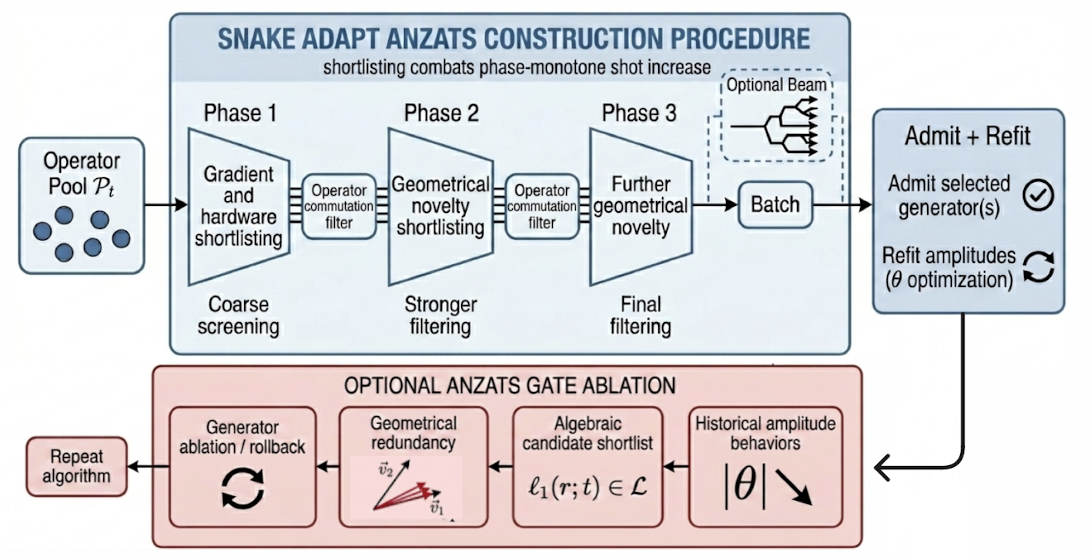
\includegraphics[width=\columnwidth]{figures/static_adapt_selector_flow_attached.png}
\captionof{figure}{SNAKE static ADAPT generator-selection flow. The broad generator pool is reduced through staged gradient--cost scoring, commutation filtering, algebraic identity shortlisting, final batch-compatible record selection, beam branching for degenerate batches, and post-admission generator-ablation.}
\label{fig:static_adapt_selector_flow}
\end{center}

\label{sec:static_method}

\subsection{Staged generator-position ranking}
%
At ADAPT iteration \(k\), \textsc{SNAKE} evaluates candidate insertions on the current ordered ansatz \(U_k(\boldsymbol\theta_k)\). In append-only ADAPT, each candidate is specified only by a generator. \textsc{SNAKE} instead represents each candidate as a generator--position record.
\[
r = (m,p),
\]
%
where \(m\) indexes the candidate generator \(A_m\in\mathcal{G}\), and \(p\) is an admissible insertion position in the current circuit.
%$\Gset=\{A_a\}_{a=1}^{|\Gset|}$ and the admissible insertion-position set $\Pcal_k=\left\{
%p\in W(\theta_k)
%\;\middle|\;
%W(\theta_k)\subseteq\{1,\ldots,|U_k(\theta_k)|+1\}
%\right\}$ where $W(\theta_k)$ is the rolling window of admissible insertion positions of the existing ordered ansatz. Define the mapping
%[
%\textcolor{red}{NO NEED TO INTRODUCE A MAPPING HERE
%\begin{equation}
%\Phi_k:(\Gset,\Pcal_k)\longrightarrow
%\mathcal R
%=
%\{r=(m,p)\mid A_m\in\Gset,\;p\in\Pcal_k\},
%\label{eq:record_mapping}
%\end{equation}
%}
%]\\
%
The candidate generator--position record set at the current iteration is then defined as follows:
\[
\mathcal{R}_k = \{ r=(m,p)\mid A_m\in\mathcal{G},\;p\in\Pcal_k\}
\label{record_set}
\]
%
where \(\Pcal_k\) is the set of possible insert positions of candidates for the ansatz at iteration \(k\). To avoid applying the expensive geometric and curvature evaluations to every record in the set, \textsc{SNAKE} ranks candidates through a staged restriction procedure. We first initialize the staged recursion set as follows
\[
\mathcal R_k^{(-1)} := \mathcal{R}_k
\]
and then apply a sequence of scoring phases indexed by \(t\in\{0,1,2,3\}\). Within each phase, records are partitioned into three lanes \(\ell\in\mathcal L\), defined by the cartesian product of qubit-support overlap and whether the candidate generator \(A_m\) commutes with a subset of generator entries of $U(\boldsymbol{\theta})$. Each phase maps the previous staged-recursion set \(\mathcal R_k^{(t-1)}\) to \(\mathcal R_k^{(t)}\) by lane-wise score thresholding or a lane-wise top-scored $N_\ell$-retained-record subset:
%\textcolor{red}{NOT SURE ABOUT $\ell$ DEPENDENCE HERE - WE MUST BE PRECISE WITH THE MATHEMATICAL DEFINITIONS}
%
\begin{equation}
\begin{aligned}
\mathcal R_k^{(t)}
:=
 \bigcup_{\ell\in\mathcal L} \Bigl[
&\left\{
r\in\mathcal R_k^{(t-1)}
\;\middle|\;
S_{t,\ell}(r)\ge\tau_{t,\ell}\right\} \\
&{}\cup \operatorname{Top}_{N_\ell}(\mathcal{R}_{k,\ell}^{(t-1)};S_{t,\ell}) \Bigr].
\end{aligned}
\label{eq:phase_restriction_map}
\end{equation}
%
The phase score at a specific lane \(\ell\) and phase \(t\) for a candidate \(r\) is defined as
%
\begin{equation}
S_{t,\ell}(r)
=
\frac{\Delta E_t(r)\mathcal N_t(r)}{K_t(r)}\,,
\label{eq:master_phase_score}
\end{equation}
\(\Delta E_t(r)\) is the phase-\(t\) state-gradient gain, \(0\leq\mathcal N_t(r)\leq 1\) is the geometric novelty factor, which down-weights candidates whose tangent direction is redundant with directions already available in the ansatz. \(K_t(r) \geq 1\) is the hardware-cost penalty. \(\tau_{t,\ell}\) is a phase- and lane-dependent threshold determined by candidate-record inter-competition. Equation~\eqref{eq:master_phase_score} generalizes append-only ADAPT's gradient ranking from a single generator score to a record-level ranking that combines estimated energy gain, novelty, and cost normalization.\\
The resulting ansatz update is written as:
%
\begin{equation}
U_{k+1}(\boldsymbol\theta_{k+1})
=
U_k(\boldsymbol\theta_{k})
\oplus
\bigcup_{r_i\in\mathcal B\subseteq\mathcal R_k^{(3)}}r_i
\ominus
\bigcup_{d_j\in\mathcal D\subseteq U_k(\boldsymbol\theta_k)}d_j .
\label{eq:snake_ansatz_update}
\end{equation}
%
Here $\mathcal B$ is the batch-admissible set of retained Phase-III records, and $\mathcal D$ is the ablation-admissible set of existing ansatz entries. Before discussing in detail the different stages of candidate selection, we will explain how the hardware cost penalty and candidate gradients are computed in the next two sections.

\subsubsection{Hardware cost penalty}
%
\noindent
The hardware-cost penalty \(K_t(r)\) estimates the additional circuit and measurement burden introduced by selecting a new candidate record \(r\). This penalty is used to avoid selecting candidates that slightly improve the energy at the cost of a substantially larger circuit depth, two-qubit gate count, parameter space dimension, or measurement cost. We include five cost components in its definition: two-qubit gate count, layout-aware two-qubit depth, one-qubit basis-change work, additional variational parameters, and grouped-measurement shot demand.\\
\noindent
For a system of \(Q\) qubits, fix a candidate record \(r=(m,p)\). The associated compiled generator is expressed as a Pauli polynomial,

\begin{equation}
A_m=\sum_{\mu}c_{\mu}P_{\mu}, \qquad P_{\mu}\in\{I,X,Y,Z\}^{\otimes Q}\,.
\label{eq:pauli_expansion}
\end{equation}
%
For each nonzero Pauli word, we define its qubit support as
%
\begin{equation}
\begin{aligned}
S_{\mu}
&:=\operatorname{supp}(P_{\mu}) \\
&=\{q\in\{1,\ldots,Q\}:(P_{\mu})_q\ne I\}.
\end{aligned}
\label{eq:pauli_word_support}
\end{equation}
%
The cost estimates below are computed from these Pauli-word supports. Larger supports require longer parity-computation circuits, while supports spread across the hardware graph require larger entangling depth or routing overhead. For a Pauli exponential compiled by a CNOT ladder, a multi-qubit Pauli rotation is implemented by reducing it to a single-qubit rotation with additional entangling gates. A Pauli word acting on \(s=|S_{\mu}|\) qubits requires \(s-1\) \textsc{CNOT}s before the \(R_z\) rotation and \(s-1\) \textsc{CNOT}s after it to restore the original qubit register. The two-qubit gate count is estimated by
%
\begin{equation}
\widehat C_{\twq}(r)=\sum_{\mu}2\,\max[|S_{\mu}|-1, 0],
\label{eq:pauli_2count_proxy}
\end{equation}
whereas the layout-aware two-qubit depth is given by
\begin{equation}
\widehat C_d(r)=\sum_{\mu}2\,\operatorname{span}_{G}
\bigl(S_{\mu}\bigr)\,.
\label{eq:pauli_2depth_proxy}
\end{equation}
Here \(G\) is the QPU connectivity graph, and $\operatorname{span}_{G}(S_{\mu})$ is the number of edges in the shortest connected subgraph containing the support \(S_{\mu}\). The quantity is set to zero when $|S_{\mu}|\le1$. This term penalizes Pauli words whose active qubits are far apart in the connected graph.\\
\noindent
The same Pauli-rotation circuit also uses one-qubit basis-change gates. Let
\[
S_{\mu}^{XY} = \{q\in S_{\mu}:(P_{\mu})_q = X\text{ or }Y\}
\]
On each qubit in \(S_{\mu}^{XY}\), we rotate into the \(Z\) basis before the Pauli rotation and rotate it back afterward. If the required basis rotation is $\beta_{\mu q}$, its forward and back cost is
\[
c_q^{\pm}(\beta_{\mu q})=c_q(\beta_{\mu q})+c_q(\beta^{-1}_{\mu q})\,.
\]
The one-qubit cost of this Pauli word is then given by
%
\begin{equation}
\widehat{C}_{1q}^{(\mu)}(r) = \sum_{q\in S_{\mu}^{XY}}c_q^\pm(\beta_{\mu q}) + c_{\bar{q}_{\mu}}(R_z)\,.
\end{equation}
%
%and let \(\beta_{m\mu q}\in\{\beta_X,\beta_Y\}\) denote the basis change required when \((P_{m\mu})_q\in\{X,Y\}\). Then
%\begin{equation}
%\begin{aligned}
%\widehat C_{1q}(r)
%=
%\sum_{\mu}
%\Bigg[
%\sum_{\substack{q:\\(P_{m\mu})_q\in\{X,Y\}}}
%c_q^{\pm}(\beta_{m\mu q})
%+
%\mathbf 1_{|S_{m\mu}|>0}c_{q_{m\mu}}(R_z)
%\Bigg],
%\end{aligned}
%\label{eq:pauli_1count_proxy}
%\end{equation}
Here \(\bar{q}_{\mu}\) is the qubit where the central rotation \(R_z\) is applied. The total one-qubit cost then becomes \(\widehat{C}_{1q}(r)=\sum_\mu\widehat{C}_{1q}^{(\mu)}(r)\). The parameter cost is the number of new independent parameters added by candidate \(r\):
%where $c_q(g)$ is the native one-qubit cost assigned to gate $g$ on vertex $q$, and $q_{m\mu}\in S_{m\mu}$ is the ladder vertex carrying the central rotation.
%
\begin{equation}
\widehat C_\theta(r)
=
|\theta\oplus\vartheta_r|-|\theta|.
\label{eq:parameter_cost_proxy}
\end{equation}
%
For single generator insertion, this is one; however, batched or tied insertions may add a different number of independent parameters. The measurement cost is computed from the candidate-gradient\cite{Verteletskyi2020CliqueCover,Yen2020CompatibleMeasurements}
\[
O_r:=i[\widetilde A_r,H]\,,
\]
after qubit mapping \(O_r\) is rewritten as a sum of Pauli words 
%
\[
O_r=\sum_{\nu=1}^{N_r}c_{r\nu}P_{r\nu}\,.
\]
%
The Pauli words are then grouped into qubit-wise commuting blocks, denoted by \(\Pi_r\), so that all Pauli words in the same block can be measured using a single basis. The goal is to estimate the additional number of shots required by candidate \(r\). Let \(\mathcal M\) be the set of measurement bases that have already been used in previous scoring steps. A block \(C\in\Pi_r\) has zero additional basis cost if it can be measured in one of these cached bases. We then denote \(C_r\subseteq\Pi_r\) as the set of such cached blocks. As a consequence, only the blocks in \(\Pi_r\setminus C_r\) require a new measurement basis.
%with \(m_q\) the measured Pauli axis on qubit \(q\). The cached-basis blocks are
%\begin{equation}
%\begin{aligned}
%\mathcal C_r
%=
%\{C\in\Pi_r:\;&
%\exists m\in\mathcal M\;
%\forall \nu\in C\;
%\forall q,\\
%&
%(P_{r\nu})_q=I
%\ \lor\
%(P_{r\nu})_q=m_q
%\}.
%\end{aligned}
%\label{eq:cached_measurement_blocks}
%\end{equation}
For each new block \(C\), we assign the coefficient weight
\[
w_C = \sqrt{\sum_{\nu\in C}|c_{r\nu}|^2}\,.
\]
The shot-cost proxy is then given by
\begin{equation}
\widehat C_{\rm shot}(r)=
\frac{1}{\sigma_\star^2}
\left[
\sum_{C\in\Pi_r\setminus C_r}
w_C
\right]^2\,.
\label{eq:shot_cost_proxy}
\end{equation}
%
Here $\sigma_\star$ is the target standard error for the candidate-gradient estimate \cite{Ikhtiarudin2025ShotEfficient}. This proxy gives a lower cost to candidates whose gradient reuses existing measurement bases and a higher cost to candidates that require new measurement blocks with large Pauli coefficients.\\
For a given cost term component $\widehat C_x$, the normalized excess cost is given by
%
\begin{equation}
\bar C_x(r;t):=
\operatorname{asinh}
\left(
\frac{\text{max}[\widehat C_x(r)-m_x(t), 0]}{s_x(t)}
\right),
\label{eq:cost_robust_excess}
\end{equation}
%
Thus, a candidate is penalized only when its cost exceeds the phase-(t) median. The inverse-hyperbolic-sine transform keeps the penalty approximately linear for moderate excess costs while compressing very large outliers\cite{IglewiczHoaglin1993,Burbidge1988IHS}.
The phase-(t) hardware-cost penalty then is one plus the weighted sum of these robust-normalized excess costs,
\begin{equation}
\begin{aligned}
K_t(r)
={}&
1+\lambda_{\twq}\bar C_{\twq}(r;t)
+\lambda_d \bar C_d(r;t)\\
&+\lambda_{1q}\bar C_{1q}(r;t)
 +\lambda_\theta \bar C_\theta(r;t)\\
&+\lambda_{\rm shot}\bar C_{\rm shot}(r;t)\,.
\end{aligned}
\label{eq:hardware_cost_sum}
\end{equation}
%
Each barred quantity in Eq.~(\ref{eq:cost_robust_excess}) is the robust excess version of the corresponding raw proxy: two-qubit gate count, layout-aware depth, one-qubit basis-change cost, parameter cost, and shot cost. The weights \(\lambda_{2Q}\),\(\lambda_d\),\(\lambda_{1q}\),\(\lambda_\theta\),\(\lambda_{\rm shot}\) instead set the relative importance of these resources.

\subsubsection{Candidate gradient}
%
\noindent
For a candidate record \(r=(m,p)\) at ADAPT iteration \(k\), the magnitude of the candidate gradient is
\begin{equation}
\begin{aligned}
g:=g(r)
&=
\left|
\left.
\partial_\alpha
\langle\psi_k|
e^{i\alpha\widetilde A_r}
H
e^{-i\alpha\widetilde A_r}
|\psi_k\rangle
\right|_{\alpha=0}
\right|\\
&=
\left|\langle\psi_k|O_r|\psi_k\rangle\right| .
\end{aligned}
\label{eq:record_gradient}
\end{equation}
%
We can now move on to discuss the different phases of the ansatz construction procedure.

\subsubsection{Phase 0}
%
\noindent
Phase 0 is the inexpensive first pass screening stage. It is obtained from Eq.~\eqref{eq:phase0_score} by using only the standard first-order ADAPT gradient and the phase-0 hardware-cost penalty. For the fixed candidate record \(r=(m,p)\), the Phase-0 score is
%
\begin{equation}
S_{0}(r)=\frac{\alpha_0 g}{K_0(r)}\,.
\label{eq:phase0_score}
\end{equation}
%
Here \(\alpha_0>0\) is a fixed pre-screening scale factor, \(g\) is the gradient magnitude from Eq.~(\ref{eq:record_gradient}), and \(K_0(r)\) is the phase-0 cost penalty. This stage is intentionally non-aggressive: its purpose is not to make the final generator-selection decision, but to remove candidates with both small gradient signals and large estimated costs before more expensive evaluations are performed. Records are passed to Phase 1 when their lane-wise score exceeds the threshold \(\tau_{0,\ell}\). To avoid discarding all useful candidates in a low-signal iteration, a fallback rule also retains the top-ranked records in each lane.

\subsubsection{Algebraic shortlisting}
%
Between scoring phases, SNAKE applies an algebraic partitioning of records for independent lane-wise scoring, where the three lanes are determined by Pauli support and whether the candidate generator commutes or does not commute with a chosen subset of the current ansatz. For a candidate record \(r=(A_m,p)\), let \(A_m\) be the candidate generator and \(p\) the proposed insertion position. Define the local comparison window

$$
\mathcal W_k(p)\subseteq\{1,\ldots,|U_k(\theta_k)|\}.
$$

whose elements index the existing ansatz generators near the proposed insertion position. Each \(n\in\mathcal W_k(p)\) labels an existing ansatz generator \(A_n\) against which the candidate \(A_m\) is compared. Comparison entails whether $A_n$ and $A_m$ share qubit support and commute. The generator-level support of $A_j$ , with
$j \in \{m, n\}$, is obtained from the union of the Pauli-word
supports in Eq.~(\ref{eq:pauli_word_support}), given by

$$
\operatorname{supp}(A_j)
:=
\bigcup_{\mu:c_{j\mu}\ne0}
\operatorname{supp}(P_{j\mu})
$$
which identifies the qubit on which the generators act non trivially.
Then \(A_m\) and \(A_n\) are support-disjoint when $\operatorname{supp}(A_m)\cap\operatorname{supp}(A_n)=\emptyset,$ and support-overlapping otherwise. On Pauli expanded candidates with joint overlapping support, we take the $L^1$ norm, which is defined by summing the absolute-valued cofficients of the Pauli polynomial after taking the commutator of $A_m$ with $A_n$. Explicitly, suppose the commutator gives
\([A_{m},A_n]
=\sum_\nu b_\nu^{}P_\nu\). Then the \(L^1\) norm is

\[
\left\|
\left[
A_{m},A_n
\right]
\right\|_1
=
\sum_\nu |b_\nu|. 
\]

Records with $\left\|
\left[
A_{m},A_n
\right]
\right\|_1 \le \epsilon$ are then assigned to the overlap commuting lane, and records greater than $\epsilon$ are assigned to the non-commuting lane.
The three lanes are thus,

$$
\ell(r)\in
\{
\mathrm{disjoint},
\mathrm{overlap\text{-}commuting},
\mathrm{overlap\text{-}noncommuting}
\}.
$$

The purpose of the three-lane shortlist is to enable more aggressive shortlists by preserving qualitatively distinct records. Within each lane, records are ordered by \(S_{t,\ell}(r)\) and thresholded by \(\tau_{t,\ell}\). The cost term \(K_t(r)\) statistics are taken over the full phase record set, not separately within each lane.

\iffalse
Between expensive scoring phases, \textsc{SNAKE} applies an algebraic shortlisting step to reduce the number of generator--position records that require subsequent evaluation. The shortlisting is based only on Pauli support and commutation information, so it can be evaluated cheaply before additional measurements are assigned. Consider a candidate record \(r=(m,p)\), where \(A_m\) is the candidate generator and \(p\) is the proposed insertion position. We define a local comparison window around \(p\)
\[
\mathcal W_k(p)\subseteq \{1,\ldots,|U_k(\theta_k)|\}\,,
\]
whose elements index the existing ansatz generators near the proposed insertion position. Each \(n\in\mathcal W_k(p)\) labels an existing generator \(A_n\) against which the candidate \(A_m\) is compared.
%sets into three lanes by defining a local algebraic comparison window $\mathcal W_k(p)\subseteq\{1,\ldots,|U_k(\theta_k)|\}$ about the insertion position of $r=(m,p)$, where each $n\in\mathcal W_k(p)$ indexes an existing ansatz generator $A_n$, and the Pauli commutation status of candidate $A_m$ with $A_n$ defines a qualitative extension or rotation action of $r$ on the variational manifold context support.
The generator-level support of $A_j$, with \(j\in\{m,n\}\), is obtained from the union of the Pauli-word supports in Eq.~(\ref{eq:pauli_word_support})
\begin{equation}
\operatorname{supp}(A_j) :=\bigcup_{\mu:c_{j\mu}\ne 0}
\operatorname{supp}(P_{j\mu}),
\label{eq:macro_generator_support}
\end{equation}


and identify the qubits on which the generators act non trivially. Two generators are support-disjoint if their total supports do not overlap, \(\operatorname{supp}(A_m)\cap\operatorname{supp}(A_n)=\emptyset\), and they are support-overlapping otherwise. For each generator indexed by \(n,m\), \textsc{SNAKE} evaluates the Pauli commutation after the expansion into Pauli words. The commutation test uses the standard parity rule: two Pauli words commute when the number of sites on which their non-identity Pauli letters anticommute is even, and anticommute when this number is odd. Generator-level commutation is then assigned based on the Pauli words commutation structure. Using this support and commutation analysis, candidate records are assigned to three algebraic lanes
\[
\ell\in
\{
\mathrm{disjoint},
\mathrm{overlap\text{-}commuting},
\mathrm{overlap\text{-}noncommuting}
\}
\]
The purpose of this three-lane shortlist is to decrease retained total candidates by increasing lane-wise shortlisting while preventing qualitatively different records from competing under a single global threshold. Within each lane, records remain ordered by the current phase score \(S_{t,\ell}(r)\), and the shortlist is obtained by applying the lane-specific threshold $\tau_{t,\ell}$. The cost-term, $K_t(r)$,  has its robust median evaluated over the entire phase record set and is lane independent. The surviving records are then passed to the next scoring phase.
\fi

\paragraph*{Inverse Notation.}
%All inverse solves below use the damped, supported version of the displayed block. For Gram blocks, \(G^+\) denotes the Moore--Penrose inverse on the retained tangent support. We suppress explicit inverse-regularization terms in the displayed scoring equations.
Some of the scores below require inverses of Gram, metric, or Hessian matrices. These matrices may be singular when the local tangent space contains redundant directions or when a candidate generator has a very little effect on the current state. Therefore, every inverse below should be understood as a regularized pseudoinverse. We use \(G^+\) for the Moore-Penrose pseudoinverse after removing numerically null directions. The same convention is used for metric and Hessian matrices. To keep the equations readable, we avoid writing the damping and projection steps explicitly.

\subsubsection{Phase I}
%
\noindent
Phase I replaces the purely gradient-based prescreening with a geometry-normalized local energy-gain estimate. For a fixed candidate record \(r\), the ADAPT gradient is evaluated together with the Fubini--Study norm of the candidate tangent\cite{Nocedal2006TrustRegion}; we suppress the \(r\)-dependence of \(g\), \(F\), \(\tau\), and \(\alpha^\star\) in this local model. In this way, phase I estimates how much the candidate record \(r\) can lower the energy before it displaces the current variational state beyond a certain value \(\rho\). The candidate is assigned a trial amplitude \(\alpha\); for each value of \(\alpha\) \textsc{SNAKE} estimates the energy-gain \(\Delta E_{1}(r)\) using a one-dimensional quadratic descriptor. The allowed values of \(\alpha\) are then restricted by the condition that the Fubini--Study displacement does not exceed \(\rho\),
%
\begin{equation}
\begin{split}
\Delta E_{1}(r)={}&\max_{\alpha^2F\le \rho^2} \left[g\alpha-\frac{1}{2}F\alpha^2\right],
\end{split}
\label{eq:phase1_gain}
\end{equation}
%
where \(g\) is given by Eq.~(\ref{eq:record_gradient}). The factor \(F\) measures how strongly candidate record \(r\) moves the current variational state. To define it, let \(\Pi=I-\ket{\psi}\bra{\psi}\) be the projector onto the subspace orthogonal to the current state. If candidate record \(r\) is admitted, it introduces a new variational parameter \(\vartheta_r\). The tangent along this coordinate in state space is \(\tau=\partial_{\vartheta_r}\ket{\psi}\). The diagonal Fubini--Study scale is then given by
%
\begin{equation}
F=\|\Pi\tau\|^2.
\label{eq:phase1_tangent_scale}
\end{equation}
%
The parameter maximizer in Eq.~(\ref{eq:phase1_gain}) is then defined by taking the following minimum
\begin{equation}
\alpha^\star
=
\min\!\left(
\dfrac{g}{F},
\dfrac{\rho}{\sqrt{F}}
\right)\,.
\label{eq:phase1_alpha_star}
\end{equation}
The value is then used to obtain the phase I gain \(\Delta E_1(r)\), which is subsequently used in the phase I score \(S_1(r)\). If the candidate is finally admitted to the ansatz, \(\alpha^\star\) is used only as an initial value. The corresponding new variational coordinate \(\vartheta_r\), together with the active ansatz parameters, is still optimized under the chosen inner optimization procedure in Eq.~\ref{eq:theta_opt}.

\subsubsection{Phase II}

The top-ranked records from phase I then pass into Phase II, which refines the local quadratic trust-region energy model with second-order curvature, and weights candidates using a novelty bonus based on whether the local ansatz tangent span can express the candidate's induced tangent. 

The trust-region constrained second-order energy estimate is given by
\begin{equation}
\Delta E_{2}(r)
=\max_{|\alpha|\sqrt{F}\le\rho}
\Bigl[g\alpha -\frac{h\alpha^2}{2}\Bigr],
\label{eq:phase2_gain}
\end{equation}
where the directional energy curvature is
\begin{align}
h&=
2\Re\!\left[
(\partial_{\alpha}\langle \psi|)H|\partial_{\alpha}\psi\rangle
+\langle\psi|H|\partial^2_{\alpha}\psi\rangle
\right],
\label{eq:phase2_hessian}
\end{align}
  
and $\partial^2_{\alpha}\ket{\psi} =-(U_{>p}A_mU_{>p}^{\dagger})^2\ket{\psi}.$ Here \(>p\) denotes the ansatz generators to the left of position index \(p\), where the right-most generator is index \(1\). In implementation, only positive curvature is retained. The trial amplitude used is the same as Eq.~\ref{eq:phase1_alpha_star} under the substitution of $g/F \to g / h$, whereas $\rho/\sqrt{F}$ remains the same, and warm-starts the newly inserted generator coordinate for admitted records.

For \(r\), let \(W_r\) be the capped reduced-geometry refit-coordinate window, with \(i,j\in W_r\). The Fubini--Study Gram matrix on this coordinate block and the candidate tangent-covariance vector are given by
\begin{equation*}
(G)_{ij}=\Re\langle\tau_i,\tau_j\rangle,
\qquad
(q)_i=\Re\langle\tau_i,\tau\rangle.
\end{equation*}
The Phase-II novelty term is the normalized least-squares component of the candidate tangent lying outside the \(W_r\)-tangent span:
\begin{equation}
\begin{aligned}
\mathcal N_2(r)
&:=
\frac{1}{F}
\min_{\gamma}
\left\|
\Pi\left(\tau-\sum_{i\in W_r}\gamma_i\tau_i\right)
\right\|^2 \\
&=
1-
\frac{q^{\top}G^+q}{F}.
\end{aligned}
\label{eq:phase2_novelty}
\end{equation}
Thus $\mathcal N_2(r)$ is small when the \(W_r\)-tangent span already contains $\tau$, and large when the candidate contributes an independent state-space direction.

\subsubsection{Generator Pauli-Splitting}
For generator records retained by the Phase-II shortlist, \textsc{SNAKE}
employs a qubit-ADAPT-VQE-style Pauli splitting to enumerate
hardware-efficient ansatz generators \cite{Tang2021}. For the parent record
\(r=(m,p)\), let
\(r_J=((m,J),p)\) define a subset of the Pauli-word support of \(A_m\). Then let
\(A_{m,J}\) be given by
\begin{equation}
A_{m,J}=\sum_{\mu\in J}c_{\mu}P_{\mu}.
\label{eq:pauli_child_generator}
\end{equation}
Since \(A_{m,J}\) is formed from a subset of the Pauli words in \(A_m\),
\(\operatorname{supp}(A_{m,J})\subseteq\operatorname{supp}(A_m)\). A fermionic
sector-preserving gate \(\Gamma(A_J)\) is then applied, which tests for the
commutation-resolved Pauli-coefficient \(L^1\) norm of the child generator
\(A_{m,J}\) with respect to both the spin-resolved and total fermionic particle
number operators. \(\Gamma(A_J)\) permits records \(r_J\) whose
\(L^1\) commutation-resolved norm is below a given threshold. Explicitly,
\begin{equation}
\Gamma(A_J)
=
\prod_{i\in\{\uparrow,\downarrow,\mathrm{total}\}}
\mathbf 1
\left\{
\left\|
\left[
A_{m,J},\mathbf N_i^{(f)}\otimes \mathbb I^{(b)}
\right]
\right\|_1
\le \epsilon
\right\}.
\label{eq:symmetry_guard}
\end{equation}
Here \(\mathbf N_i^{(f)}\) is the fermionic number operator for spin up, spin
down, or total particle number; We tensor \(\mathbf N_i^{(f)}\) with the boson
register identity operator. Here \(\epsilon\) is a runtime leakage-tolerance
parameter.
\iffalse
The Pauli-coefficient \(L^1\) norm is defined by summing the absolute
coefficients of the Pauli polynomial after taking the commutator in
Eq.~\eqref{eq:symmetry_guard}. Explicitly, suppose the commutator gives
\([A_{m,J},\mathbf N_i^{(f)}\otimes \mathbb I^{(b)}]
=\sum_\nu b_\nu^{(i,J)}P_\nu\). Then the \(L^1\) norm is
\[
\left\|
\left[
A_{m,J},\mathbf N_i^{(f)}\otimes \mathbb I^{(b)}
\right]
\right\|_1
=
\sum_\nu |b_\nu^{(i,J)}|.
\]

\fi
These symmetry-retained operator-children then act as the new shortlisted
operator set for subsequent Phase-III scoring and batching. We omit explicit
\(J\)-dependence below for visual simplicity, and assume all records
\(r=(m,p)\) may be Pauli-word combinations with subset generator support of a
parent generator \(A_m\).
\subsubsection{Phase III}

Phase III performs Schur-refit reranking over candidate-specific refit-coordinate windows.

The energy gain model is
\begin{equation}
\Delta E_{3}(r)=
\max_{|\alpha|\sqrt{F^\star}\le\rho}
\left[g\alpha-\frac{h^\star \alpha^2}{2}\right].
\label{eq:phase3_gain}
\end{equation}
Here $F^\star$ and $h^\star$ are defined in Eqs.~(\ref{eq:phase3_star_geometry}) and~(\ref{eq:phase3_schur_response}) and represent the predicted Fubini--Study metric and the energy-curvature after admitting $r$ and allowing the existing ansatz $U_k(\theta_k)$ to reoptimize. Here $\alpha^\star$ is given by Eq.~\ref{eq:phase1_alpha_star} under the substitution $g/F \to g/h^\star$ and $\rho / \sqrt{F} \to \rho / \sqrt{F^\star}$.

Let $\delta\theta$ be the response parameter vector with indices in \(W_r\subseteq\{1,\ldots,|\boldsymbol{\theta}_k|\}\). Phase III assumes a local quadratic model in which the candidate operator's energy gain is coupled to this refit-window response after admitting $r$.
Explicitly, 
\begin{equation}
\begin{split}
E(\alpha,\delta\theta)\approx{}&E_0-g\alpha+\frac{h\alpha^2}{2} \\
&+\alpha c^{\top}\delta\theta
+\frac{\delta\theta^{\top}\mathbf{H}\delta\theta}{2},
\end{split}
\label{eq:local_quadratic}
\end{equation}
where $c$ couples the candidate to the \(W_r\)-coordinate response and $\mathbf{H}$ is the corresponding Hessian block; entries are given by
\begin{equation}
\begin{aligned}
c_j&:=
\left.
\frac{\partial^2E(\alpha,\delta\theta)}
{\partial\alpha\,\partial(\delta\theta_j)}
\right|_0,\\
\mathbf{H}_{jk}&:=
\left.
\frac{\partial^2E(\alpha,\delta\theta)}
{\partial(\delta\theta_j)\,\partial(\delta\theta_k)}
\right|_0,
\qquad j,k\in W_r .
\end{aligned}
\label{eq:phase3_window_derivatives}
\end{equation}
Let \(\mathbf R\) denote the symmetrized \(W_r\)-supported Hessian block used in the refit solve:
\begin{equation}
\mathbf R=\frac12(\mathbf H+\mathbf H^{\top}).
\label{eq:phase3_regularized_hessian}
\end{equation}

Eliminating the \(W_r\) coordinates by optimizing Eq.~\ref{eq:local_quadratic} over $\delta\theta$ gives the optimal local refit response induced by the candidate, and substituting it back into Eq.~(\ref{eq:local_quadratic}) yields the Schur-relaxed curvature $h^\star$. Explicitly,
\begin{equation}
\delta\theta^\star=-\alpha\mathbf R^{-1}c,
\qquad
h^\star=h-c^{\top}\mathbf R^{-1}c .
\label{eq:phase3_schur_response}
\end{equation}
Equations (\ref{eq:phase3_window_derivatives})–(\ref{eq:phase3_regularized_hessian}) give the ideal Schur model; the inverse and damping convention is the one stated above
and also applies to the batch Schur blocks below. Evaluating $\delta\theta^\star$ at the selected trial amplitude $\alpha^\star$ gives the inherited-coordinate warm-start seed for the inner re-optimization on the enlarged ansatz. Dividing $\delta\theta^\star$ by $\alpha$ gives the inherited-coordinate compensation per unit candidate amplitude. This defines the Schur-reduced residual tangent, Schur-reduced Fubini--Study norm, and Schur-reduced candidate--ansatz overlap:
\begin{equation}
\begin{aligned}
\tau^\star
&=\tau+\sum_{i\in W_r}\left(\frac{\delta\theta^\star}{\alpha}\right)_i\tau_i,\\
F^\star
&=F+2q^{\top}\frac{\delta\theta^\star}{\alpha}
+\frac{(\delta\theta^\star)^{\top}}{\alpha}G\frac{\delta\theta^\star}{\alpha},\\
q^\star
&=q+G\frac{\delta\theta^\star}{\alpha}.
\end{aligned}
\label{eq:phase3_star_geometry}
\end{equation}
This completes Eq.~(\ref{eq:phase3_gain}), and enables a least-squares treatment, analogous to Eq.~(\ref{eq:phase2_novelty}), to define a Phase-III novelty factor:
\begin{equation}
\begin{aligned}
\mathcal N_3(r)
&:=
\frac{1}{F^\star}
\min_{\gamma}
\left\|
\Pi\left(\tau^\star-\sum_{i\in W_r}\gamma_i\tau_i\right)
\right\|^2 \\
&=
1-\frac{(q^\star)^{\top}G^+q^\star}
{F^\star}.
\end{aligned}
\label{eq:phase3_novelty}
\end{equation}

\subsubsection{Batching}
For a set of records that survived Phase III scores, defined by Eq.~(\ref{eq:phase_restriction_map}), define the set of eligible batch candidates to be $B\subseteq\mathcal R_k^{(3)}$.  An optional conservative batch shortlist restricts \(B\) to records with disjoint qubit support and mutual commutation.

For batch-local indices \(a,b=1,\ldots,s\) and capped batch refit-coordinate window \(W_B\), let $H_{BB}=[\partial_{\alpha_a}\partial_{\alpha_b}E]_{a,b=1}^s$ be the Hessian block among candidate amplitudes, and let $H_{W_BB}=[\partial_{\theta_i}\partial_{\alpha_a}E]_{i\in W_B,\,a=1,\ldots,s}$ be the mixed window-candidate block. Then, with $H_{W_BW_B}=[\partial_{\theta_i}\partial_{\theta_j}E]_{i,j\in W_B}$ and $\mathbf R_B=\frac12(H_{W_BW_B}+H_{W_BW_B}^{\top})$, the Schur-refit batch curvature, residual tangents, and reduced Gram matrix are
\begin{equation}
\begin{aligned}
H_B^\star
&=
H_{BB}
-
H_{BW_B}\mathbf R_B^{-1}H_{W_BB},\\
\tau_a^\star
&=\tau_a-\sum_{i\in W_B}(\mathbf R_B^{-1}H_{W_BB})_{ia}\tau_i,\\
(G_B^\star)_{ab}
&=\Re\langle \Pi\tau_a^\star,\Pi\tau_b^\star\rangle .
\end{aligned}
\label{eq:batch_schur_curvature}
\end{equation}

For an induced gradient vector of $B$, define \(g_B=\big(g_{r_1},\ldots,g_{r_s}\big)^\top\). This enables an expected batch gain,
\begin{equation}
\Delta E_3(B)
=
\max_{\alpha_B^\top G_B^\star\alpha_B\le \rho_B^2}
\left[
g_B^\top\alpha_B
-
\frac12\alpha_B^\top H_B^\star\alpha_B
\right],
\label{eq:batch_expected_gain}
\end{equation}
The admitted batch is therefore
\begin{equation}
B^\star\in\arg\max_{B\subseteq\mathcal R_k^{({3)}}}\frac{\Delta E_3(B)}{K_3(B)}.
\label{eq:batch_argmax}
\end{equation}
Equation~(\ref{eq:batch_argmax}) is the combinatorial search ideal, although a score-ordered greedy admission serves as a measurement-cheap practical approximation. 

\subsubsection{Beaming}
\textsc{SNAKE} borrows Lowerre-style beam search to branch candidate circuits in parallel \cite{Lowerre1976Beam}.. Given a score-ordered top-$N$ candidate-batch list, a parent circuit can spawn $N$ child branches, with each child differing by the batched candidate admitted to that branch. The cost of this parallel beam universe is increased total hardware-graph and qubit support across candidate child circuits. Each child branch then undergoes the generator-ablation procedure described next. Under a fixed beam capacity, branch retention and termination follow the hardware-cost-weighted energy-dominance ordering among child branches.


\subsubsection{Generator ablation}
Generator ablation acts after a generator is admitted and the inner optimizer
refits the current ansatz.  We propose an objective given by
Eq.~\eqref{eq:schur_metric_prune} which models the Schur response energy and
state-displacement response of the ansatz circuit under removal of a candidate
generator.  Write the current ansatz circuit at iteration \(k\) as
\[
U_k(\boldsymbol\theta_k^\star)
=
\prod_{i=1}^{n_k}\exp(\theta_{k,i}^\star A_i).
\]
Define its ordered generator sequence as
\[
\mathbf A_k=(A_1,\ldots,A_{n_k}).
\]
Each active generator \(A_j\) carries an admission step \(a_j\) and a cooldown
counter \(c_j(k)\).  Equivalently, if \(\hat r_j\) is the most recent rejected
delete/refit trial for \(A_j\), a fixed cooldown requires
\(k-\hat r_j\ge\tilde c\); if no such rejection exists, the cooldown condition
is satisfied.  The deletion-eligible coordinates are
\begin{equation}
\mathcal E_k^\ominus
=
\left\{
j\in\{1,\ldots,n_k\}
:
k-a_j\ge \tilde p,\;
c_j(k)\le0
\right\}.
\label{eq:eligibility_set}
\end{equation}
Here \(\tilde p\) and \(\tilde c\) are run-time constant protection thresholds.

Then, for \(j\in\mathcal E_k^\ominus\), we predict the Schur response energy
loss under the ablation of \(A_j\), together with the ability of the ansatz to
recover the pre-ablation state by minimizing the Fubini--Study metric
displacement.  Define the surviving ansatz-generator index set as
\[
D:=\{1,\ldots,n_k\}\setminus\{j\},
\qquad
|D|=n_k-1 .
\]
Let \(u,v\in D\) denote surviving-coordinate indices.  All quantities below are
evaluated at \(U_k(\boldsymbol\theta_k^\star)\):
\[
\tau_u
=
\left.
\partial_{\theta_u}\ket{\psi(U_k,\boldsymbol\theta)}
\right|_{\boldsymbol\theta=\boldsymbol\theta_k^\star},
\qquad
G_{uv}
=
\operatorname{Re}\langle \Pi_k^\star\tau_u,\Pi_k^\star\tau_v\rangle,
\]
\[
g_u
=
\left.
\partial_{\theta_u}E(U_k,\boldsymbol\theta)
\right|_{\boldsymbol\theta=\boldsymbol\theta_k^\star},
\qquad
H_{uv}
=
\left.
\partial_{\theta_u}\partial_{\theta_v}E(U_k,\boldsymbol\theta)
\right|_{\boldsymbol\theta=\boldsymbol\theta_k^\star}.
\]

We define the metric-regularized Schur ablation surrogate as
\begin{equation}
\begin{aligned}
\Lambda(A_j)
=
\min_{\delta\theta_D}
\Biggl[
&\Lambda_E(A_j,\delta\theta_D)
\\
&+
\frac{\eta}{2}
\left\|
\Pi_k^\star
\left(
-\theta_{k,j}^\star\tau_j
+
\sum_{u\in D}\delta\theta_u\tau_u
\right)
\right\|^2
\Biggr].
\end{aligned}
\label{eq:schur_metric_prune}
\end{equation}
The local energy term is the deletion specialization of the Phase-III
quadratic model in Eq.~\eqref{eq:local_quadratic}:
\begin{equation}
\begin{aligned}
\Lambda_E(A_j,\delta\theta_D)
={}&
-g_j\theta_{k,j}^\star
+
\frac12(\theta_{k,j}^\star)^2H_{jj}
\\
&-
\theta_{k,j}^\star H_{Dj}^{\top}\delta\theta_D
+
\frac12\delta\theta_D^{\top}H_{DD}\delta\theta_D .
\end{aligned}
\label{eq:lambda_schur_energy_loss}
\end{equation}
The parameter \(\eta\ge0\) controls the Fubini--Study regularization of the
ablation Schur model.  Equivalently, define the metric-regularized quadratic
block
\[
\mathcal Q:=H+\eta G .
\]
The optimal Schur response becomes
\begin{equation}
\begin{aligned}
\delta\boldsymbol\theta_D^\star
&=
\theta_{k,j}^\star
\mathcal Q_{DD}^{+}\mathcal Q_{Dj}
\\
&=
\theta_{k,j}^\star
\left(H_{DD}+\eta G_{DD}\right)^+
\left(H_{Dj}+\eta G_{Dj}\right).
\end{aligned}
\label{eq:ablation_schur_response}
\end{equation}
Substitution into Eq.~\eqref{eq:schur_metric_prune} gives
\begin{equation}
\begin{aligned}
\Lambda(A_j)
={}&
-g_j\theta_{k,j}^\star
+
\frac12(\theta_{k,j}^\star)^2\mathcal Q_{jj}
\\
&-
\frac12(\theta_{k,j}^\star)^2
\mathcal Q_{Dj}^{\top}
\mathcal Q_{DD}^{+}
\mathcal Q_{Dj}.
\end{aligned}
\label{eq:ablation_schur_loss}
\end{equation}

To prefer deletions that relieve larger compiled and measurement burden, let
\(K_j\) be the same normalized hardware/shot-cost denominator used in the SNAKE
candidate scores, evaluated over the current ansatz-entry population.  The
cost-weighted prune nomination score is
\[
\widetilde\Lambda(A_j)
=
\frac{\max\{0,\Lambda(A_j)\}}{K_j}.
\]
Smaller \(\widetilde\Lambda(A_j)\) is preferred.  Schur pruning therefore
nominates generators whose predicted metric-regularized deletion loss is small
relative to the hardware and estimator burden they remove.  Generator ablation
\(\mathbf A_k\ominus A_{j^\star}\) is determined by
\begin{equation}
A_{j^\star}
\in
\operatorname*{arg\,min}_{A_j\in\mathbf A_k}
\left\{
\widetilde\Lambda(A_j)
:
j\in\mathcal E_k^\ominus,\;
\widetilde\Lambda(A_j)\le\epsilon
\right\}.
\label{eq:ablation_nomination}
\end{equation}
After a candidate deletion, the acceptance gate depends on whether the energy
loss from ablation satisfies the threshold
\begin{equation}
\Delta E(A_{j^\star})
\le
\min\left\{
\epsilon,\,
\rho\left(E(U_{k-1})-E(U_k)\right)
\right\},
\label{eq:rollback_prune}
\end{equation}
where \(0\le\rho\le1\) constrains the loss to be a fraction of the most recent
admitted energy gain.

If Eq.~\eqref{eq:rollback_prune} rejects the trialed ablation, the post-refit
branch remains \(U_k(\boldsymbol\theta_k^\star)\).  This allows the Gram block results to be
reused in Eqs.~\eqref{eq:phase2_novelty}, \eqref{eq:phase3_star_geometry}, and
\eqref{eq:phase3_novelty}; similarly, the Hessian block is reused in
Eqs.~\eqref{eq:phase3_window_derivatives}--\eqref{eq:phase3_schur_response}.
The Phase-III displacement coordinates are local
shifts, \(\theta=\theta^\star+\delta\theta\), so derivatives in
\(\delta\theta\) at \(\delta\theta=0\) reuse the same \(G\) and \(H\)
subblocks.  Conversely, if Eq.~\eqref{eq:rollback_prune} accepts the ablation, subsequent Phase-II/III
scoring recomputes \(G\) and \(H\) on the refit pruned circuit
\(U_k^{\ominus}((\boldsymbol\theta_k^\star)_{\setminus j^\star})
=
U_k(\boldsymbol\theta_k^\star)\ominus
\exp(\theta_{k,j^\star}^\star A_{j^\star})\), where \((\boldsymbol\theta_k^\star)_{\setminus j^\star}\) represents the optimized circuit parameterization after removing coordinate \(j^\star\).



\subsection{Stopping condition}
The outer adaptive loop repeats phases zero through three, followed by batch, beam, and generator-ablation, until either maximum logical depth is reached, maximum compiled circuit-cost budget is saturated, or a gradient plateau below a predefined threshold persists for a patience-period-defined number of consecutive iterations.

%\end{comment} 


\section{Results}
\label{sec:results}
\label{sec:benchmarks}

We frame the advantage of SNAKE in terms of reducing energy-error and circuit-resource metrics compared to append-only ADAPT-VQE and the recently released Geo-ADAPT-VQE on an equally physically parameterized two-site Hubbard--Holstein model. 

Supplementary appendices include results for dimer lattice models of Hubbard, Bose-Hubbard, and spin-boson; we further include an instance of the three-site Hubbard--Holstein model. All fermionic-relevant models use half filling, and all lattice models use open boundary conditions. We define the operator-local pool in Appendix~\ref{app:pools}, along with the inner-optimization budgets in Appendix~\ref{app:results_discussion}. Comparisons of the three ADAPT methods use the same inner-optimization method and the same operator pool, with the exception that ADAPT-VQE is tested on the parent-generator only pool as well as the entire Pauli-child split of the initial operator set. Geo-ADAPT is shown only on the parent-pool due to non-competitive results from the child pool.

We report energy error as the absolute difference between the ADAPT-resolved lowest energy and the exact-diagonalization lowest energy, \(|\Delta E|=|E_{\rm ADAPT}-E_{\rm ED}|\), under the same phonon cutoffs. The weak-Holstein sectors use phonon cutoff \(M=2\), and the strong-Holstein sectors use \(M=4\).
In App.~\ref{app:hh_cutoff_sensitivity}, we report the effect of phonon truncation on total energy found by exact diagonalization using logarithmic change for $M\in\{1,...,10\}.$ Fidelity is reported as \(1-F=1-\left|\braket{\psi_{\rm ED}}{\psi_{\rm ADAPT}}\right|^2\).

We record $E_{\rm{ADAPT}}$ and $\ket{\psi_{\rm{ADAPT}}}$ at ADAPT iteration $k_{\rm{pl}}$, as marked on the error vs iteration plots shown below. Circuit-resource columns report the final number of two-qubit gates (\(N_{2q}\)), two-qubit depth (\(D_{2q}\)), and total circuit depth (\(D_c\)); these circuit costs are also reported at the ansatz circuit iteration \(k_{\rm pl}\), and rely on transpilation to the Qiskit IBM Marrakesh backend \cite{JavadiAbhari2024Qiskit,QiskitAlgorithmsAdaptVQE}. We report an estimator-query count (\(S\)) defined in Appendix~\ref{app:estimator_work_proxy}, which measures the total amount of logical expectation-value queries the ADAPT variant used to reach iteration \(k_{\rm pl}\); this includes candidate gradient scans, metric computations, and inner-optimizer objective evaluations.

The point \(k_{\rm pl}\) is chosen by visual inspection of diminishing energy gradients and corresponds to the initial plateau point on the error vs iteration plots shown below. We allow each method to run for \(30\) ADAPT outer-loop iterations.


%For the spin-boson/Rabi model defined in Appendix~\ref{app:spin_boson_rabi}, all three methods converged within a few iterations under similar circuit costs. We present results thereof along with the operator pool used there.

\subsection{Hubbard--Holstein benchmarks}
Using the parametrization convention given in Eq.~\eqref{eq:hubbard_holstein_static}, we report the interaction regimes in terms of \(U\), \(t\), \(g\), and \(\omega_0\).
For the Hubbard sector, we classify weak, intermediate, and strong electronic-correlation regimes using the dimer convention:

\begin{equation}
    U/t \in\{0.25,1.25,8\} \label{hubbard_regimes}
\end{equation}

Within each Hubbard correlation regime, we consider weak and strong Holstein electron--phonon coupling regimes. Using the Holstein dimer convention, \(\lambda=2g^2/(t\omega_0)\). We choose \(\omega_0/t=1\), which gives \(g/t=\sqrt{\lambda/2}\) \cite{Sakkinen2015HolsteinDimer}.
The chosen weak and strong Holstein coupling regimes are given by:

\begin{equation}
    \lambda\in\{0.25,1.25\} \label{holstein_sectors}
\end{equation}

These correspond to \(g/t=\sqrt{\lambda/2}=0.354\) and \(0.791\) in Eq.~\eqref{eq:hubbard_holstein_static}. Together these choices define six combined Hubbard--Holstein interaction regimes, obtained by crossing three Hubbard correlation regimes with two Holstein electron--phonon coupling regimes. The Cartesian product of Eqs.~\eqref{hubbard_regimes} and~\eqref{holstein_sectors} is given below for ADAPT-VQE, Geo-ADAPT, and SNAKE.


Results reported below use SciPy Powell with a max iteration budget of 200 for the inner optimization procedure of Eq.~\eqref{eq:theta_opt}; we report results of a NISQ-friendly inner optimization procedure known as simultaneous perturbation stochastic approximation (SPSA) but present those results in Appendix~\ref{app:results_discussion} so that comparisons do not depend on fine-tuning an ADAPT variant's inner-optimization schedule. 

The Pauli-children splitting of SNAKE used here allowed for singleton Pauli words to pass after the fermion symmetry gate was applied. To present fair results, we run Geo-ADAPT and ADAPT-VQE under two pool regimes: once with the parent pool only, and then once with the Pauli child-singleton pool only after the symmetry gate was applied. The Geo-ADAPT child pool results remained non-competitive and so we omitted them; Namely, the parent-generator Geo-ADAPT row had equal error in the weak--weak regime, and lower in the other five regimes, with the benefit of one to two orders of magnitude lower estimator-work \(S\).

% BEGIN_MACHINE_READABLE_HH_SNAKE_NOBATCH_DUPLICATE_PROMOTION_20260707
% {
%   "build_asset_restores": [
%     {
%       "destination": "MATH/paper_details/figures/static_adapt_selector_flow_attached.png",
%       "destination_sha256": "2d33cb0ef97858486b43c543bca6d6df1d4f170743a8940cd76ab143a03177b0",
%       "purpose": "build_enablement_only_non_hh_science_input",
%       "source": "/Users/jakestrobel/Documents/Holstein_implementation/Holstein_test_fullclone_3/MATH/paper_details/figures/static_adapt_selector_flow_attached.png",
%       "source_sha256": "2d33cb0ef97858486b43c543bca6d6df1d4f170743a8940cd76ab143a03177b0"
%     },
%     {
%       "destination": "MATH/paper_details/figures/paper_i_hubbard_weak_supportive_diagnostic_20260610.png",
%       "destination_sha256": "416d54fbae17e2bbecc6dd72b27ed49a56a5bf3bcd188170ac436458ed048647",
%       "purpose": "build_enablement_only_non_hh_science_input",
%       "source": "/Users/jakestrobel/Documents/Holstein_implementation/Holstein_test_fullclone_3/MATH/paper_details/figures/paper_i_hubbard_weak_supportive_diagnostic_20260610.png",
%       "source_sha256": "416d54fbae17e2bbecc6dd72b27ed49a56a5bf3bcd188170ac436458ed048647"
%     },
%     {
%       "destination": "MATH/paper_details/figures/paper_i_beam_tree_example.png",
%       "destination_sha256": "cc49a177de0a2c083102b3b8b2ac4b93decb0ded80446163d2127819d89045e7",
%       "purpose": "build_enablement_only_non_hh_science_input",
%       "source": "/Users/jakestrobel/Documents/Holstein_implementation/Holstein_test_fullclone_3/MATH/paper_details/figures/paper_i_beam_tree_example.png",
%       "source_sha256": "cc49a177de0a2c083102b3b8b2ac4b93decb0ded80446163d2127819d89045e7"
%     },
%     {
%       "destination": "MATH/paper_details/figures/paper_i_hubbard_weak_u0p25_append_geo_snake_overlay_20260621.png",
%       "destination_sha256": "e5c377e69fc3bf9dc0e46919348cd92d0ceb261494056db766ac4f7d050dae86",
%       "purpose": "build_enablement_only_non_hh_science_input",
%       "source": "/Users/jakestrobel/Documents/Holstein_implementation/Holstein_test_fullclone_3/MATH/paper_details/figures/paper_i_hubbard_weak_u0p25_append_geo_snake_overlay_20260621.png",
%       "source_sha256": "e5c377e69fc3bf9dc0e46919348cd92d0ceb261494056db766ac4f7d050dae86"
%     },
%     {
%       "destination": "MATH/paper_details/figures/hubbard_weak_full_noise_fixed_depth8_error_vs_iteration_20260613.pdf",
%       "destination_sha256": "a461b78977350cbf6eca61e60d855cb696d285596145f90cef5f8fe879fb3311",
%       "purpose": "build_enablement_only_non_hh_science_input",
%       "source": "/Users/jakestrobel/Documents/Holstein_implementation/Holstein_test_fullclone_3/MATH/paper_details/figures/hubbard_weak_full_noise_fixed_depth8_error_vs_iteration_20260613.pdf",
%       "source_sha256": "a461b78977350cbf6eca61e60d855cb696d285596145f90cef5f8fe879fb3311"
%     },
%     {
%       "destination": "MATH/paper_details/figures/hubbard_strong_full_noise_fixed_depth8_error_vs_iteration_20260613.pdf",
%       "destination_sha256": "74b0e69af948d7cdfd3f5a38430400379d442e017aa016f32f144cfbb7f57470",
%       "purpose": "build_enablement_only_non_hh_science_input",
%       "source": "/Users/jakestrobel/Documents/Holstein_implementation/Holstein_test_fullclone_3/MATH/paper_details/figures/hubbard_strong_full_noise_fixed_depth8_error_vs_iteration_20260613.pdf",
%       "source_sha256": "74b0e69af948d7cdfd3f5a38430400379d442e017aa016f32f144cfbb7f57470"
%     },
%     {
%       "destination": "MATH/paper_details/figures/hh_ed_cutoff_log_sensitivity_20260614.pdf",
%       "destination_sha256": "c9e9f0cb7d8baeebed238a490dbb65f7d9b1d46534ced996fea0a8ee69c4006a",
%       "purpose": "build_enablement_only_non_hh_science_input",
%       "source": "/Users/jakestrobel/Documents/Holstein_implementation/Holstein_test_fullclone_3/MATH/paper_details/figures/hh_ed_cutoff_log_sensitivity_20260614.pdf",
%       "source_sha256": "c9e9f0cb7d8baeebed238a490dbb65f7d9b1d46534ced996fea0a8ee69c4006a"
%     },
%     {
%       "destination": "MATH/paper_details/output/pdf/paper_i_true_strong_replacement_20260613_hubbard_u8_strong.pdf",
%       "destination_sha256": "2eff5d26e02d18606379901d91c523bc31ff0e434f562579881b2f782163e9e0",
%       "purpose": "build_enablement_only_non_hh_science_input",
%       "source": "/Users/jakestrobel/Documents/Holstein_implementation/Holstein_test_fullclone_3/output/pdf/paper_i_true_strong_replacement_20260613_hubbard_u8_strong.pdf",
%       "source_sha256": "2eff5d26e02d18606379901d91c523bc31ff0e434f562579881b2f782163e9e0"
%     },
%     {
%       "destination": "MATH/paper_details/output/pdf/paper_i_data_analysis_spin_boson_weak_repeat_enabled_same_cutoff_error_vs_iteration_20260610.pdf",
%       "destination_sha256": "9579065ea5c05c8f16d0c80502aa190ba2731dc4a4df2507565a778acbca1cc4",
%       "purpose": "build_enablement_only_non_hh_science_input",
%       "source": "/Users/jakestrobel/Documents/Holstein_implementation/Holstein_test_fullclone_3/output/pdf/paper_i_data_analysis_spin_boson_weak_repeat_enabled_same_cutoff_error_vs_iteration_20260610.pdf",
%       "source_sha256": "9579065ea5c05c8f16d0c80502aa190ba2731dc4a4df2507565a778acbca1cc4"
%     },
%     {
%       "destination": "MATH/paper_details/output/pdf/paper_i_data_analysis_spin_boson_strong_repeat_enabled_same_cutoff_error_vs_iteration_20260610.pdf",
%       "destination_sha256": "79dc711aff5cfa42626a3e53add324034a4e53b37f7054404010d81478ecdddb",
%       "purpose": "build_enablement_only_non_hh_science_input",
%       "source": "/Users/jakestrobel/Documents/Holstein_implementation/Holstein_test_fullclone_3/output/pdf/paper_i_data_analysis_spin_boson_strong_repeat_enabled_same_cutoff_error_vs_iteration_20260610.pdf",
%       "source_sha256": "79dc711aff5cfa42626a3e53add324034a4e53b37f7054404010d81478ecdddb"
%     }
%   ],
%   "changed_snake_cells": {
%     "intermediate-strong": {
%       "D2q": 94,
%       "Dc": 468,
%       "N2q": 132,
%       "S_alg": 82687,
%       "S_alg_source": "snake_algorithmic_work_from_payload(scope=display_prefix)",
%       "abs_delta_e": 0.0001937024882201488,
%       "d_pl": 28,
%       "fidelity_status": "unavailable",
%       "k_pl": 28,
%       "one_minus_f": null,
%       "qiskit_cost_source": "qiskit_local_snake_history_prefix_compile",
%       "result_json": "raw_outputs/paper_i_hh_powell_visible_batchroute_nobatch_20260706/intermediate_strong__snake__powell200__phase3_archival_subset1__beam0p005_metricprune__nobatch_fullv2/json/result.json",
%       "result_sha256": "4a678f07d75a6ffcc2a217549d7ebf082e8c76d5a98c673e02b2527a2173fa3d"
%     },
%     "intermediate-weak": {
%       "D2q": 36,
%       "Dc": 216,
%       "N2q": 42,
%       "S_alg": 9250,
%       "S_alg_source": "snake_algorithmic_work_from_payload(scope=display_prefix)",
%       "abs_delta_e": 0.0001720721077778098,
%       "d_pl": 13,
%       "fidelity_status": "unavailable",
%       "k_pl": 13,
%       "one_minus_f": null,
%       "qiskit_cost_source": "qiskit_local_snake_history_prefix_compile",
%       "result_json": "raw_outputs/paper_i_hh_powell_visible_batchroute_nobatch_20260706/intermediate_weak__snake__powell200__phase3_archival_subset1__beam0p005_metricprune__nobatch_fullv2/json/result.json",
%       "result_sha256": "d270becf1210f563191236ff513fdb8bfdcdbf4c9fc7d40231931334ecb344c4"
%     },
%     "strong-strong": {
%       "D2q": 31,
%       "Dc": 171,
%       "N2q": 42,
%       "S_alg": 6397,
%       "S_alg_source": "snake_algorithmic_work_from_payload(scope=display_prefix)",
%       "abs_delta_e": 4.130878044228403e-05,
%       "d_pl": 11,
%       "fidelity_status": "unavailable",
%       "k_pl": 11,
%       "one_minus_f": null,
%       "qiskit_cost_source": "qiskit_local_snake_history_prefix_compile",
%       "result_json": "raw_outputs/paper_i_hh_powell_visible_batchroute_nobatch_20260706/strong_strong__snake__powell200__phase3_archival_subset1__beam0p005_metricprune__nobatch_fullv2/json/result.json",
%       "result_sha256": "dfabad48cd3401604d3cee5cab7b3432675617338a1c3fcd1a1933060ea512dd"
%     },
%     "strong-weak": {
%       "D2q": 56,
%       "Dc": 300,
%       "N2q": 66,
%       "S_alg": 11888,
%       "S_alg_source": "snake_algorithmic_work_from_payload(scope=display_prefix)",
%       "abs_delta_e": 1.3933229825457971e-06,
%       "d_pl": 18,
%       "fidelity_status": "unavailable",
%       "k_pl": 18,
%       "one_minus_f": null,
%       "qiskit_cost_source": "qiskit_local_snake_history_prefix_compile",
%       "result_json": "raw_outputs/paper_i_hh_powell_visible_batchroute_nobatch_20260706/strong_weak__snake__powell200__phase3_archival_subset1__beam0p005_metricprune__nobatch_fullv2/json/result.json",
%       "result_sha256": "3088875ddfa7992b561f4d4b51cf33fb82e635a578a3bcbd3b08a1e317bb69b6"
%     },
%     "weak-strong": {
%       "D2q": 106,
%       "Dc": 493,
%       "N2q": 134,
%       "S_alg": 103260,
%       "S_alg_source": "snake_algorithmic_work_from_payload(scope=display_prefix)",
%       "abs_delta_e": 0.009041207759421077,
%       "d_pl": 30,
%       "fidelity_status": "computed_from_selected_prefix_fidelity",
%       "k_pl": 30,
%       "one_minus_f": 0.0035816844997489383,
%       "qiskit_cost_source": "qiskit_local_snake_history_prefix_compile",
%       "result_json": "raw_outputs/paper_i_hh_powell_visible_batchroute_nobatch_20260706/weak_strong__snake__powell200__phase3_archival_subset1__beam0p005_metricprune__nobatch_fullv2/json/result.json",
%       "result_sha256": "b6c32c2b1bc515f943650f62f2f360a5ad8ae11f639e1b70bf37b217f79a7b4d"
%     },
%     "weak-weak": {
%       "D2q": 33,
%       "Dc": 178,
%       "N2q": 42,
%       "S_alg": 8012,
%       "S_alg_source": "snake_algorithmic_work_from_payload(scope=display_prefix)",
%       "abs_delta_e": 0.00039160562082241057,
%       "d_pl": 12,
%       "fidelity_status": "unavailable",
%       "k_pl": 12,
%       "one_minus_f": null,
%       "qiskit_cost_source": "qiskit_local_snake_history_prefix_compile",
%       "result_json": "raw_outputs/paper_i_hh_powell_visible_batchroute_nobatch_20260706/weak_weak__snake__powell200__phase3_archival_subset1__beam0p005_metricprune__nobatch_fullv2/json/result.json",
%       "result_sha256": "ee696a09816d99c07cf4ca82e165848ea6cfee55eb7014ee45e2c2491ca45262"
%     }
%   },
%   "comparator_policy": "Geo/Append rows and trajectories retained from 20260702 POWELL pool-exposure support artifacts",
%   "duplicate_tex": "MATH/paper_details/static_adapt_paper_I_snake_nobatch_promoted_20260707.tex",
%   "fidelity_policy": "display 1-F only if selected-prefix fidelity is source-computable; otherwise --",
%   "optimizer": "POWELL",
%   "plot_files": {
%     "intermediate_strong": {
%       "pdf": "MATH/paper_details/figures/powell_snake_nobatch_promoted_20260707/paper_i_hh_snake_nobatch_promoted_20260707__intermediate_strong.pdf",
%       "pdf_sha256": "0c3cb45e7a577f635131ae16d3eabb58a9af0e3a02565bf0ad9bab1d90ac101f",
%       "png": "MATH/paper_details/figures/powell_snake_nobatch_promoted_20260707/paper_i_hh_snake_nobatch_promoted_20260707__intermediate_strong.png",
%       "png_sha256": "34ca942f394dec788b876191b6aefddd620ca9fa9b55295663f56e89af56e7ef"
%     },
%     "intermediate_weak": {
%       "pdf": "MATH/paper_details/figures/powell_snake_nobatch_promoted_20260707/paper_i_hh_snake_nobatch_promoted_20260707__intermediate_weak.pdf",
%       "pdf_sha256": "4b854ae931b71ef618423433fe926d956891e87d63b7beaffe541aff37b9bb35",
%       "png": "MATH/paper_details/figures/powell_snake_nobatch_promoted_20260707/paper_i_hh_snake_nobatch_promoted_20260707__intermediate_weak.png",
%       "png_sha256": "e7273fd2008a611dc9a1dbb367d48a2647e064fa8463a09625b03358853f57fd"
%     },
%     "strong_strong": {
%       "pdf": "MATH/paper_details/figures/powell_snake_nobatch_promoted_20260707/paper_i_hh_snake_nobatch_promoted_20260707__strong_strong.pdf",
%       "pdf_sha256": "461c2be27ebd3c9ca79c5e2404614b28a1dadd15bb834cb7e3a61f19e2163803",
%       "png": "MATH/paper_details/figures/powell_snake_nobatch_promoted_20260707/paper_i_hh_snake_nobatch_promoted_20260707__strong_strong.png",
%       "png_sha256": "b21f5fd50dfa21ecec8f28546e7ff426ea504a87aae85d5fd73a546039b7eb19"
%     },
%     "strong_weak": {
%       "pdf": "MATH/paper_details/figures/powell_snake_nobatch_promoted_20260707/paper_i_hh_snake_nobatch_promoted_20260707__strong_weak.pdf",
%       "pdf_sha256": "4dea776b8ea92bd822f06b62bbead7dbca43f696e53b8834a8b0bc61604f3ec5",
%       "png": "MATH/paper_details/figures/powell_snake_nobatch_promoted_20260707/paper_i_hh_snake_nobatch_promoted_20260707__strong_weak.png",
%       "png_sha256": "e99cbc377c9403352226bfdaa35208e43f4880a009c92c2d11a864f68ca05990"
%     },
%     "weak_strong": {
%       "pdf": "MATH/paper_details/figures/powell_snake_nobatch_promoted_20260707/paper_i_hh_snake_nobatch_promoted_20260707__weak_strong.pdf",
%       "pdf_sha256": "409779d66bf309bc501e69220d720edb5261c641aac12f449cfe593da6c72b9f",
%       "png": "MATH/paper_details/figures/powell_snake_nobatch_promoted_20260707/paper_i_hh_snake_nobatch_promoted_20260707__weak_strong.png",
%       "png_sha256": "59ef2b53ada0943bdfcfffd2883ed553dcaf897217d4c4629c9a58dc12fcc865"
%     },
%     "weak_weak": {
%       "pdf": "MATH/paper_details/figures/powell_snake_nobatch_promoted_20260707/paper_i_hh_snake_nobatch_promoted_20260707__weak_weak.pdf",
%       "pdf_sha256": "bf1a290bdb23c216a80bbd3357f047a4d742f09e84cc8fc69192b4562990d5bf",
%       "png": "MATH/paper_details/figures/powell_snake_nobatch_promoted_20260707/paper_i_hh_snake_nobatch_promoted_20260707__weak_weak.png",
%       "png_sha256": "27cbc20956cd5907d1fd1502702b5c1b396e619c3e0e7bc4f2436fd0f67623c3"
%     }
%   },
%   "qiskit_circuit_scope": "ansatz_circuit_including_reference_state",
%   "qiskit_compile_convention": "table_i_basis_gate_transpile_v1",
%   "retained_comparator_source_csv": "/Users/jakestrobel/Documents/Holstein_implementation/Holstein_test_fullclone_3/output/pdf/paper_i_hh_fullmeta_singleton_symmetry_chtc_current_20260630/paper_i_hh_fullmeta_singleton_symmetry_chtc_current_20260630_powell_pool_exposure_support.csv",
%   "retained_comparator_source_json": "/Users/jakestrobel/Documents/Holstein_implementation/Holstein_test_fullclone_3/output/pdf/paper_i_hh_fullmeta_singleton_symmetry_chtc_current_20260630/paper_i_hh_fullmeta_singleton_symmetry_chtc_current_20260630_powell_pool_exposure_support.json",
%   "row_policy": "promote only latest local no-batch SNAKE rows; preserve existing Geo/Append cells",
%   "s_alg_policy": "row-facing winner-lineage/display-prefix S_alg; not S_beam_search_total",
%   "schema": "paper_i_hh_snake_nobatch_duplicate_promotion_v1",
%   "scope": "duplicate_only; SNAKE rows and HH plots updated; original manuscript untouched",
%   "snake_runtime_contract": {
%     "adapt_beam_children_per_parent": 2,
%     "adapt_beam_lambda": 0.005,
%     "adapt_beam_live_branches": 3,
%     "batching_enabled": false,
%     "metric_prune_route": true,
%     "pool": "full_meta_unfiltered_hva_included",
%     "runtime_split_max_subset_size": 1,
%     "runtime_split_mode": "shortlist_pauli_children_v1",
%     "runtime_split_selection": "archival_child_set_forward_v1"
%   },
%   "source_csv": "output/pdf/paper_i_hh_powell_visible_batchroute_nobatch_vs_paper1_snake_20260707/paper_i_hh_powell_visible_batchroute_nobatch_vs_paper1_snake_20260707_provenance.csv",
%   "source_hashes": {
%     "/Users/jakestrobel/Documents/Holstein_implementation/Holstein_test_fullclone_3/output/pdf/paper_i_hh_fullmeta_singleton_symmetry_chtc_current_20260630/paper_i_hh_fullmeta_singleton_symmetry_chtc_current_20260630_powell_pool_exposure_support.csv": "6409dd077cb4ab0fceaa15d62e7570a70549a49f1ed9989abcea6435767c521c",
%     "/Users/jakestrobel/Documents/Holstein_implementation/Holstein_test_fullclone_3/output/pdf/paper_i_hh_fullmeta_singleton_symmetry_chtc_current_20260630/paper_i_hh_fullmeta_singleton_symmetry_chtc_current_20260630_powell_pool_exposure_support.json": "eb18dc3e62d9db8654612232a4841895042f4794be236ff06d3533698bafc15f",
%     "/Users/jakestrobel/Documents/Holstein_implementation/Holstein_test_fullclone_3/output/pdf/paper_i_hh_fullmeta_singleton_symmetry_chtc_current_20260630/paper_i_hh_fullmeta_singleton_symmetry_chtc_current_20260630_powell_pool_exposure_support.pdf": "4fee45db46167eea19181fc5b8fc1e73f23240c25982e5bc766b0c21c8734a02",
%     "MATH/paper_details/static_adapt_paper_I.tex": "98ea34779d3fe58329590d7832d02ec0244358a81a66be55182a5913a0dfe54d",
%     "output/pdf/paper_i_hh_powell_visible_batchroute_nobatch_vs_paper1_snake_20260707/paper_i_hh_powell_visible_batchroute_nobatch_vs_paper1_snake_20260707.pdf": "9a9babb4cb6caa9aaece4dc11139f0c1c4e8da0b7b012e71a87340b1923b39ed",
%     "output/pdf/paper_i_hh_powell_visible_batchroute_nobatch_vs_paper1_snake_20260707/paper_i_hh_powell_visible_batchroute_nobatch_vs_paper1_snake_20260707_provenance.csv": "af9e9ad917da0538ab018e90dffa48ebfa637439d9f4a69ad1d36d0ea8fd7844",
%     "output/pdf/paper_i_hh_powell_visible_batchroute_nobatch_vs_paper1_snake_20260707/paper_i_hh_powell_visible_batchroute_nobatch_vs_paper1_snake_20260707_provenance.json": "9b3128f5b0bfa8914491596516ea0d96cc91cb5d62cd125945b8227bed901427"
%   },
%   "source_json": "output/pdf/paper_i_hh_powell_visible_batchroute_nobatch_vs_paper1_snake_20260707/paper_i_hh_powell_visible_batchroute_nobatch_vs_paper1_snake_20260707_provenance.json",
%   "source_pdf": "output/pdf/paper_i_hh_powell_visible_batchroute_nobatch_vs_paper1_snake_20260707/paper_i_hh_powell_visible_batchroute_nobatch_vs_paper1_snake_20260707.pdf",
%   "source_tex": "MATH/paper_details/static_adapt_paper_I.tex",
%   "supersedes_for_snake_rows": [
%     "BEGIN_MACHINE_READABLE_HH_POWELL_POOL_EXPOSURE_MAIN_UPDATE_20260702",
%     "BEGIN_MACHINE_READABLE_HH_POWELL_POOL_EXPOSURE_SNAKE_RUNTIME_SPLIT_TRACE_20260705",
%     "older HH native200/Schur/SNAKE provenance blocks in the duplicate"
%   ],
%   "updated_date": "2026-07-07",
%   "validation": {
%     "non_snake_comparator_rows_identical_to_source_tex": {
%       "intermediate_strong": true,
%       "intermediate_weak": true,
%       "strong_strong": true,
%       "strong_weak": true,
%       "weak_strong": true,
%       "weak_weak": true
%     },
%     "rows": {
%       "intermediate_strong": {
%         "tex_row": "SNAKE & 28 & 1.937e-04 & -- & 132 & 94 & 468 & 82,687 \\\\",
%         "validated": true
%       },
%       "intermediate_weak": {
%         "tex_row": "SNAKE & 13 & 1.721e-04 & -- & 42 & 36 & 216 & 9,250 \\\\",
%         "validated": true
%       },
%       "strong_strong": {
%         "tex_row": "SNAKE & 11 & 4.131e-05 & -- & 42 & 31 & 171 & 6,397 \\\\",
%         "validated": true
%       },
%       "strong_weak": {
%         "tex_row": "SNAKE & 18 & 1.393e-06 & -- & 66 & 56 & 300 & 11,888 \\\\",
%         "validated": true
%       },
%       "weak_strong": {
%         "tex_row": "SNAKE & 30 & 9.041e-03 & 3.582e-03 & 134 & 106 & 493 & 103,260 \\\\",
%         "validated": true
%       },
%       "weak_weak": {
%         "tex_row": "SNAKE & 12 & 3.916e-04 & -- & 42 & 33 & 178 & 8,012 \\\\",
%         "validated": true
%       }
%     },
%     "source_tex_hash_unchanged": true
%   }
% }
% END_MACHINE_READABLE_HH_SNAKE_NOBATCH_DUPLICATE_PROMOTION_20260707

\noindent\begin{minipage}{\columnwidth}
\begin{center}
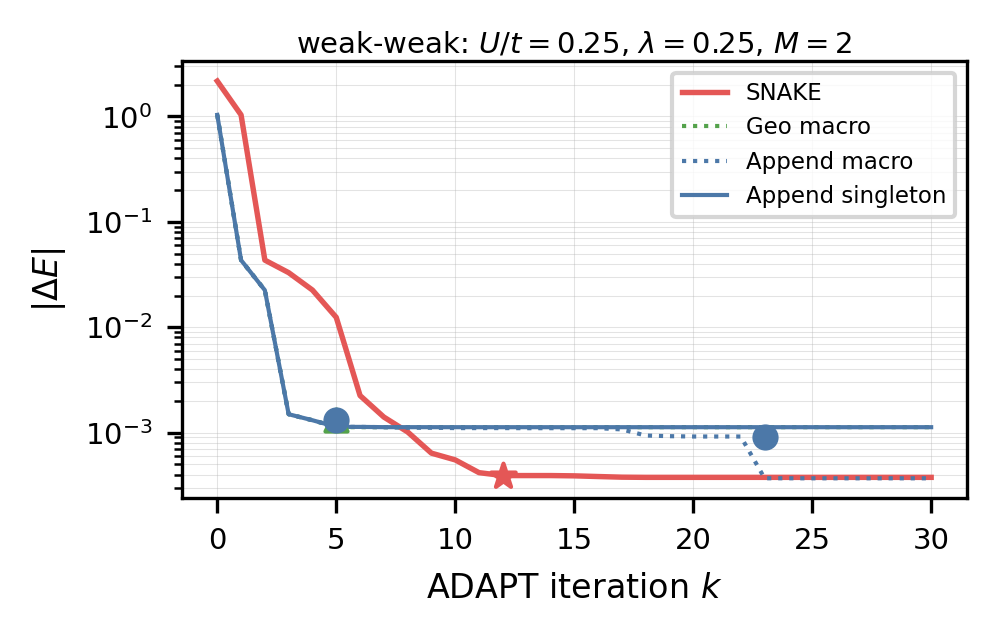
\includegraphics[width=\columnwidth]{figures/powell_snake_nobatch_promoted_20260707/paper_i_hh_snake_nobatch_promoted_20260707__weak_weak.png}
\end{center}
\end{minipage}
\par\addvspace{0.35ex}

\noindent\begin{minipage}{\columnwidth}
\begin{center}
\scriptsize
\setlength{\tabcolsep}{0.70pt}
\renewcommand{\arraystretch}{1.0}
\textit{weak--weak: $(U/t,\lambda)=(0.25,0.25)$, \(M=2\)}
\par\smallskip
\begin{ruledtabular}
\begin{tabular}{p{0.205\columnwidth}ccccccc}
Method & \metrichead{$k_{\rm pl}$} & \metrichead{$|\Delta E|$} & \metrichead{$1-F$} & \metrichead{$N_{\twq}$} & \metrichead{$D_{\twq}$} & \metrichead{$D_c$} & \metrichead{$S$}\\
\colrule
SNAKE & 12 & 3.916e-04 & -- & 42 & 33 & 178 & 8,012 \\
Geo macro & 5 & 1.312e-03 & -- & 98 & 67 & 480 & 24,859 \\
% Omitted Geo singleton source row: Geo singleton & 5 & 1.312e-03 & -- & 98 & 70 & 539 & 466,828 \\
Append macro & 23 & 9.193e-04 & -- & 4,216 & 4,033 & 15,936 & 108,633 \\
\shortstack[l]{Append\\singleton} & 5 & 1.312e-03 & -- & 98 & 70 & 534 & 3,129 \\
\end{tabular}
\end{ruledtabular}
\end{center}
\end{minipage}
\par\addvspace{0.45ex}

\noindent\begin{minipage}{\columnwidth}
\begin{center}
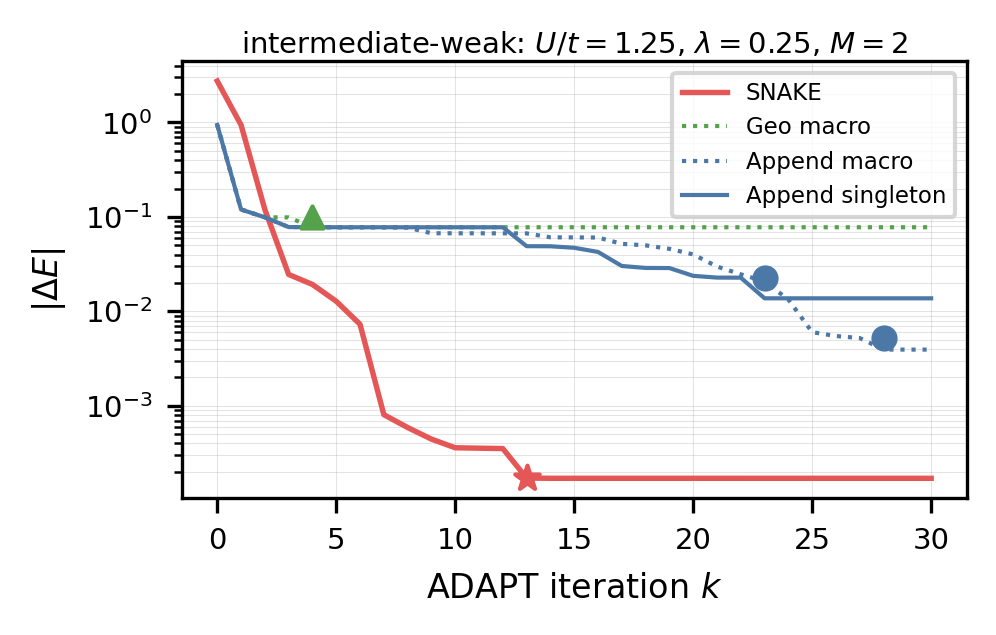
\includegraphics[width=\columnwidth]{figures/powell_snake_nobatch_promoted_20260707/paper_i_hh_snake_nobatch_promoted_20260707__intermediate_weak.png}
\end{center}
\end{minipage}
\par\addvspace{0.35ex}

\noindent\begin{minipage}{\columnwidth}
\begin{center}
\scriptsize
\setlength{\tabcolsep}{0.70pt}
\renewcommand{\arraystretch}{1.0}
\textit{intermediate--weak: $(U/t,\lambda)=(1.25,0.25)$, \(M=2\)}
\par\smallskip
\begin{ruledtabular}
\begin{tabular}{p{0.205\columnwidth}ccccccc}
Method & \metrichead{$k_{\rm pl}$} & \metrichead{$|\Delta E|$} & \metrichead{$1-F$} & \metrichead{$N_{\twq}$} & \metrichead{$D_{\twq}$} & \metrichead{$D_c$} & \metrichead{$S$}\\
\colrule
SNAKE & 13 & 1.721e-04 & -- & 42 & 36 & 216 & 9,250 \\
Geo macro & 4 & 9.893e-02 & -- & 70 & 69 & 528 & 19,792 \\
% Omitted Geo singleton source row: Geo singleton & 2 & 0.12 & -- & 40 & 40 & 285 & 186,863 \\
Append macro & 28 & 5.224e-03 & -- & 4,276 & 4,059 & 15,924 & 231,208 \\
\shortstack[l]{Append\\singleton} & 23 & 2.277e-02 & -- & 562 & 485 & 2,374 & 134,322 \\
\end{tabular}
\end{ruledtabular}
\end{center}
\end{minipage}
\par\addvspace{0.45ex}

\noindent\begin{minipage}{\columnwidth}
\begin{center}
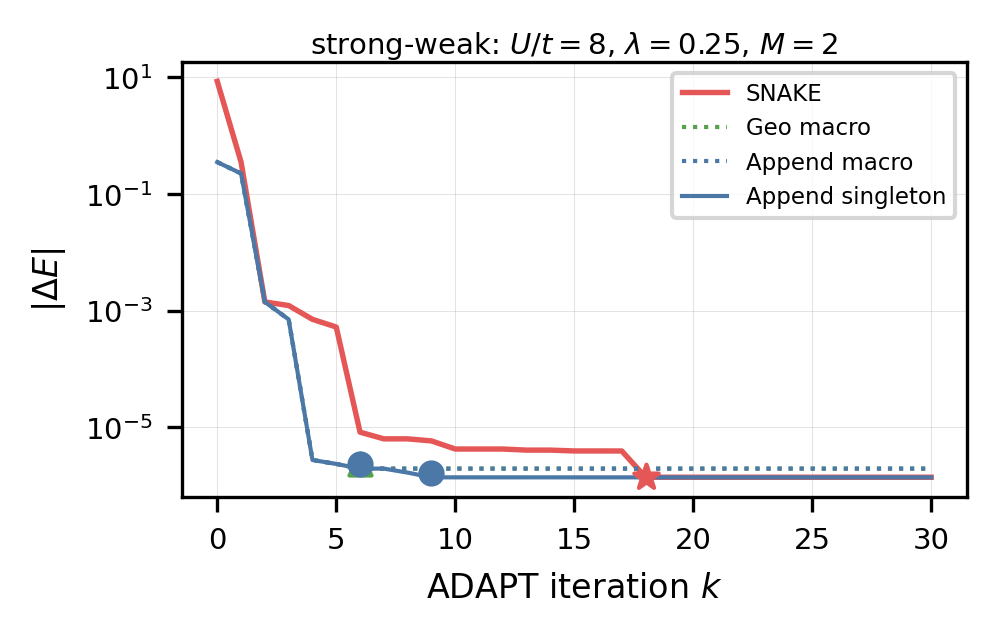
\includegraphics[width=\columnwidth]{figures/powell_snake_nobatch_promoted_20260707/paper_i_hh_snake_nobatch_promoted_20260707__strong_weak.png}
\end{center}
\end{minipage}
\par\addvspace{0.35ex}

\noindent\begin{minipage}{\columnwidth}
\begin{center}
\scriptsize
\setlength{\tabcolsep}{0.70pt}
\renewcommand{\arraystretch}{1.0}
\textit{strong--weak: $(U/t,\lambda)=(8,0.25)$, \(M=2\)}
\par\smallskip
\begin{ruledtabular}
\begin{tabular}{p{0.205\columnwidth}ccccccc}
Method & \metrichead{$k_{\rm pl}$} & \metrichead{$|\Delta E|$} & \metrichead{$1-F$} & \metrichead{$N_{\twq}$} & \metrichead{$D_{\twq}$} & \metrichead{$D_c$} & \metrichead{$S$}\\
\colrule
SNAKE & 18 & 1.393e-06 & -- & 66 & 56 & 300 & 11,888 \\
Geo macro & 6 & 2.355e-06 & -- & 146 & 117 & 763 & 30,007 \\
% Omitted Geo singleton source row: Geo singleton & 4 & 7.064e-04 & -- & 116 & 116 & 710 & 373,478 \\
Append macro & 6 & 2.355e-06 & -- & 146 & 118 & 762 & 2,137 \\
\shortstack[l]{Append\\singleton} & 9 & 1.672e-06 & -- & 156 & 126 & 814 & 7,310 \\
\end{tabular}
\end{ruledtabular}
\end{center}
\end{minipage}
\par\addvspace{0.45ex}

\noindent\begin{minipage}{\columnwidth}
\begin{center}
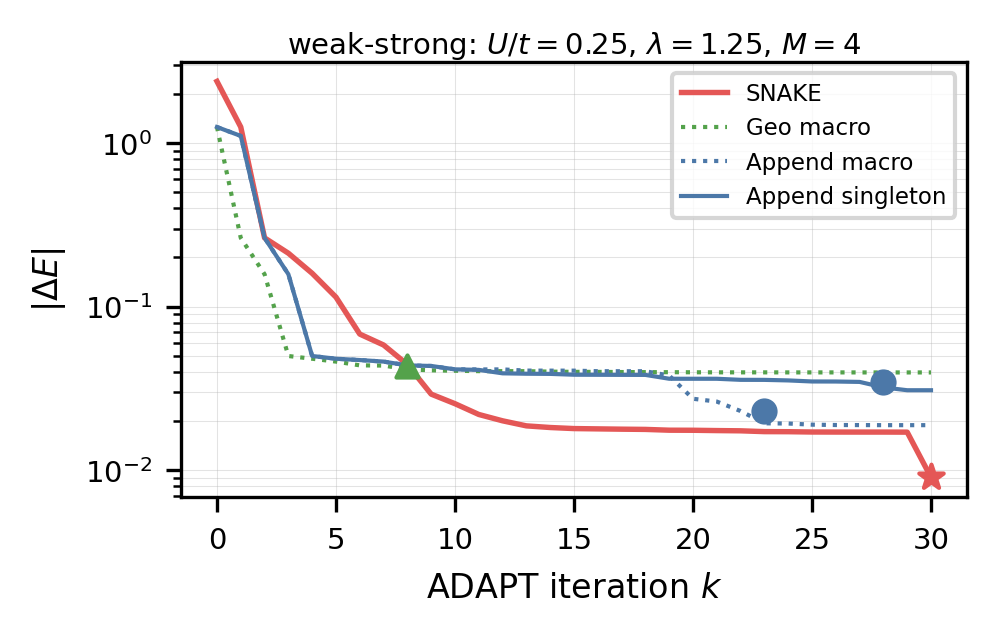
\includegraphics[width=\columnwidth]{figures/powell_snake_nobatch_promoted_20260707/paper_i_hh_snake_nobatch_promoted_20260707__weak_strong.png}
\end{center}
\end{minipage}
\par\addvspace{0.35ex}

\noindent\begin{minipage}{\columnwidth}
\begin{center}
\scriptsize
\setlength{\tabcolsep}{0.70pt}
\renewcommand{\arraystretch}{1.0}
\textit{weak--strong: $(U/t,\lambda)=(0.25,1.25)$, \(M=4\)}
\par\smallskip
\begin{ruledtabular}
\begin{tabular}{p{0.205\columnwidth}ccccccc}
Method & \metrichead{$k_{\rm pl}$} & \metrichead{$|\Delta E|$} & \metrichead{$1-F$} & \metrichead{$N_{\twq}$} & \metrichead{$D_{\twq}$} & \metrichead{$D_c$} & \metrichead{$S$}\\
\colrule
SNAKE & 30 & 9.041e-03 & 3.582e-03 & 134 & 106 & 493 & 103,260 \\
Geo macro & 8 & 4.365e-02 & -- & 1,784 & 1,641 & 6,160 & 47,155 \\
% Omitted Geo singleton source row: Geo singleton & 4 & 0.157 & -- & 280 & 280 & 1,610 & 2,728,149 \\
Append macro & 23 & 2.301e-02 & -- & 32,596 & 31,946 & 94,899 & 136,947 \\
\shortstack[l]{Append\\singleton} & 28 & 3.468e-02 & -- & 27,400 & 27,169 & 77,949 & 228,209 \\
\end{tabular}
\end{ruledtabular}
\end{center}
\end{minipage}
\par\addvspace{0.45ex}

% Duplicate-only layout guard: keep the last two HH plot/table pairs in the same visual column.
\newpage
\noindent\begin{minipage}{\columnwidth}
\begin{center}
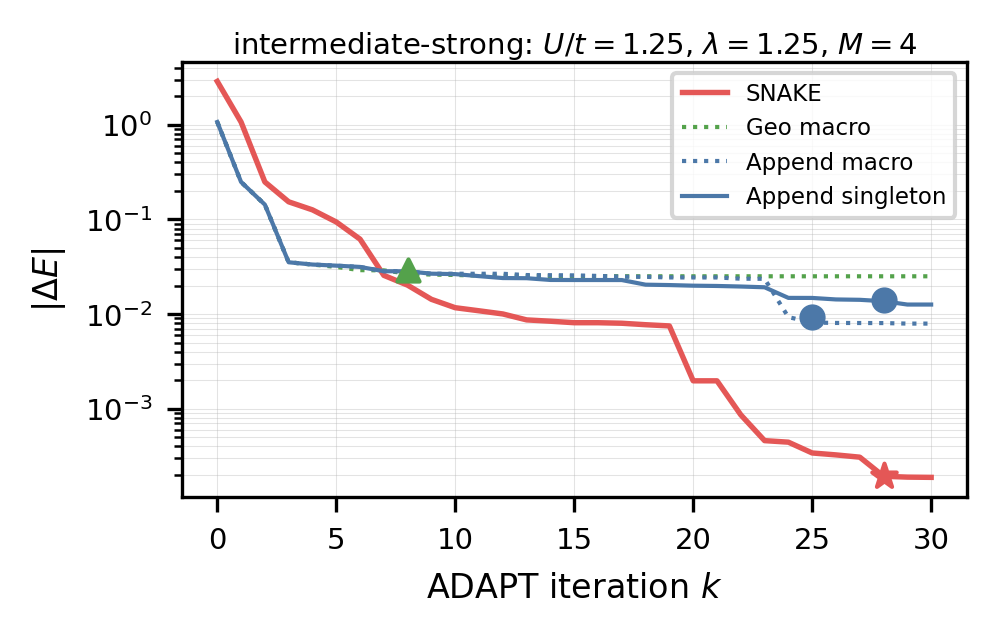
\includegraphics[width=\columnwidth]{figures/powell_snake_nobatch_promoted_20260707/paper_i_hh_snake_nobatch_promoted_20260707__intermediate_strong.png}
\end{center}
\end{minipage}
\par\addvspace{0.35ex}

\noindent\begin{minipage}{\columnwidth}
\begin{center}
\scriptsize
\setlength{\tabcolsep}{0.70pt}
\renewcommand{\arraystretch}{1.0}
\textit{intermediate--strong: $(U/t,\lambda)=(1.25,1.25)$, \(M=4\)}
\par\smallskip
\begin{ruledtabular}
\begin{tabular}{p{0.205\columnwidth}ccccccc}
Method & \metrichead{$k_{\rm pl}$} & \metrichead{$|\Delta E|$} & \metrichead{$1-F$} & \metrichead{$N_{\twq}$} & \metrichead{$D_{\twq}$} & \metrichead{$D_c$} & \metrichead{$S$}\\
\colrule
SNAKE & 28 & 1.937e-04 & -- & 132 & 94 & 468 & 82,687 \\
Geo macro & 8 & 2.898e-02 & -- & 1,784 & 1,632 & 6,104 & 47,245 \\
% Omitted Geo singleton source row: Geo singleton & 2 & 0.249 & -- & 40 & 40 & 285 & 1,364,468 \\
Append macro & 25 & 9.296e-03 & -- & 33,340 & 32,457 & 97,248 & 167,416 \\
\shortstack[l]{Append\\singleton} & 28 & 1.416e-02 & -- & 32,782 & 32,239 & 96,144 & 247,019 \\
\end{tabular}
\end{ruledtabular}
\end{center}
\end{minipage}
\par\addvspace{0.45ex}

\noindent\begin{minipage}{\columnwidth}
\begin{center}
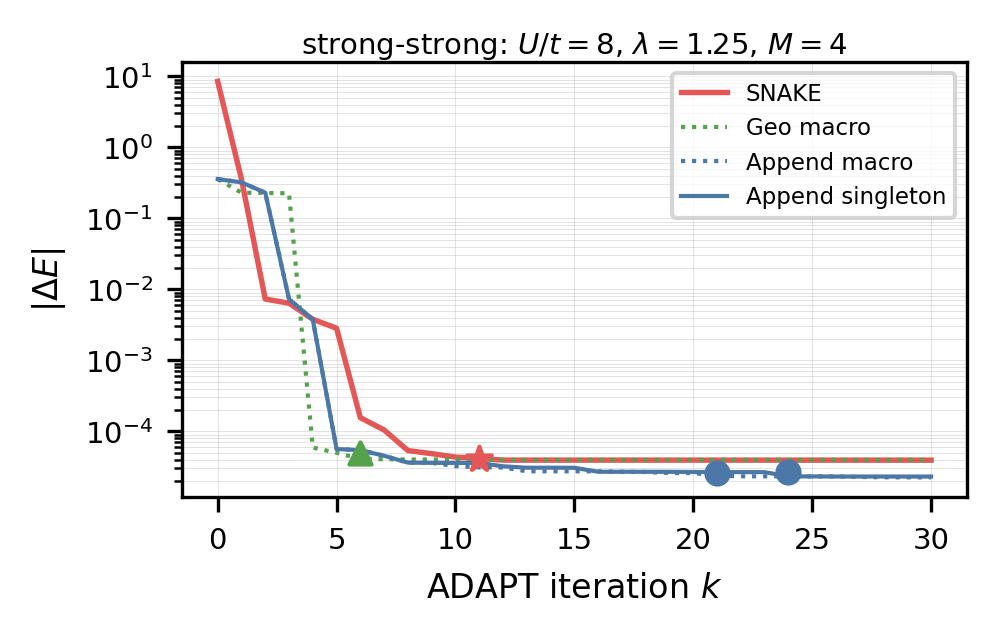
\includegraphics[width=\columnwidth]{figures/powell_snake_nobatch_promoted_20260707/paper_i_hh_snake_nobatch_promoted_20260707__strong_strong.png}
\end{center}
\end{minipage}
\par\addvspace{0.35ex}

\noindent\begin{minipage}{\columnwidth}
\begin{center}
\scriptsize
\setlength{\tabcolsep}{0.70pt}
\renewcommand{\arraystretch}{1.0}
\textit{strong--strong: $(U/t,\lambda)=(8,1.25)$, \(M=4\)}
\par\smallskip
\begin{ruledtabular}
\begin{tabular}{p{0.205\columnwidth}ccccccc}
Method & \metrichead{$k_{\rm pl}$} & \metrichead{$|\Delta E|$} & \metrichead{$1-F$} & \metrichead{$N_{\twq}$} & \metrichead{$D_{\twq}$} & \metrichead{$D_c$} & \metrichead{$S$}\\
\colrule
SNAKE & 11 & 4.131e-05 & -- & 42 & 31 & 171 & 6,397 \\
Geo macro & 6 & 4.982e-05 & -- & 348 & 206 & 1,149 & 33,962 \\
% Omitted Geo singleton source row: Geo singleton & 4 & 3.736e-03 & -- & 208 & 208 & 1,170 & 2,727,920 \\
Append macro & 21 & 2.577e-05 & -- & 32,600 & 31,931 & 94,541 & 73,566 \\
\shortstack[l]{Append\\singleton} & 24 & 2.654e-05 & -- & 32,234 & 31,714 & 93,028 & 89,870 \\
\end{tabular}
\end{ruledtabular}
\end{center}
\end{minipage}
\par\addvspace{0.45ex}
% BEGIN_DRAFT_HH_CHILD_FAIRNESS_PROSE_TODO_20260624
% Condensed future-prose note; comment only, do not render yet.
% Use the native-forced SPSA Pauli-child protocol as the main displayed HH comparison.
% Treat monotone/non-forced rows as sensitivity evidence: Append and Geo improve under monotone,
% while SNAKE is stronger in the native-forced child+Schur condition or comparable to monotone.
% No-child SNAKE hurts under the current parameterization; phrase this as a hyperparameter/
% Optuna/settings limitation, not as an intrinsic limitation of SNAKE.
% Schur warm-start versus no-Schur warm-start did not materially change same-cutoff
% energy error in this comparison; treat Schur as a refit/conditioning and cost-shaping
% mechanism unless a later source-locked replay shows an accuracy separation.
% Candidate claim: native-forced SNAKE child+Schur versus Geo monotone no-child gives
% same-order aggregate same-cutoff energy accuracy with much smaller SNAKE compiled circuit cost.
% Shot/work costs remain pending under a common accounting convention.
% Avoid overclaiming: strong--weak is the visible outlier in the compact comparison.
% Source support: output/pdf/paper_i_hh_child_fairness_20260623/
% paper_i_hh_child_fairness_compact_child_schur_20260623.{pdf,json,csv}.
% END_DRAFT_HH_CHILD_FAIRNESS_PROSE_TODO_20260624
\par\addvspace{1.0ex}
\clearpage

% BEGIN_MACHINE_READABLE_WEAK_WEAK_SCHUR_LADDER_POSTER_ABLATION_MATRICES_20260622
% {"schema":"paper_i_weak_weak_schur_ladder_poster_ablation_matrices_v2","updated_date":"2026-06-23","table_labels":["tab:weak_weak_schur_ladder_ablation_plateau_percent","tab:weak_weak_schur_ladder_ablation_terminal_percent"],"support_json":"MATH/paper_facing/paper_I_static_scaffold/paper_i_weak_weak_schur_ladder_poster_ablation_matrices_20260622.json","support_json_sha256":"4a5414596d16c5c4c3fcbdee83482cc3528180602869be08ad26c2eade3a4993","source_json":"output/pdf/paper_i_hh_weak_weak_schur_ladder_ablation_delta_report_20260621.json","source_json_sha256":"59cce4ab0ee046b3b3b607ea353fa8cb3c7bec18948c8ddf21836d7d5fd85730","poster_tex":"/Users/jakestrobel/Downloads/SNAKE_UW_Poster_PRISM_Upload_work/SNAKE_UW_Poster.tex","poster_tex_sha256":"21e32a2d32a18bbc9be3a840d45d45bd66c29f651fd119e16568325f6d63056c","poster_asset_provenance_json":"/Users/jakestrobel/Downloads/SNAKE_UW_Poster_PRISM_Upload_work/assets/ablation_schur_ladder_percent_matrix_provenance.json","poster_asset_provenance_sha256":"f62b9faee5c2be44994e087f68bf657a91ce939f4536386f8d209871c5081c0e","benchmark":"weak--weak Hubbard--Holstein","comparison":"percent change versus full SNAKE anchor","row_policy":"no-shortlisting rendered as a placeholder row pending corrected deterministic-shot rerun","plateau_placeholder_policy":"plateau-prefix Delta L_D, Delta(1-F), and Delta S are visible placeholders until recomputed","terminal_fidelity_note":"terminal percent fidelity-loss changes are copied from the main poster TeX block; source JSON used for error/cost columns does not carry terminal fidelity fields"}
% END_MACHINE_READABLE_WEAK_WEAK_SCHUR_LADDER_POSTER_ABLATION_MATRICES_20260622
\noindent\begin{minipage}{\columnwidth}
\captionof{table}{\label{tab:weak_weak_schur_ladder_ablation_plateau_percent}Weak--weak Hubbard--Holstein SNAKE mechanism ablations at the plateau prefix. All $\Delta$ columns are percent changes relative to the full-SNAKE anchor; \(k_{\rm pl}\) is the accepted-prefix index. Negative $\Delta|\Delta E|$ means a lower energy error than the anchor, whereas positive resource changes mean larger circuit or estimator burden. Placeholder entries mark plateau-prefix \(L_D\), \(1-F\), and \(S\) values awaiting recomputation.}
\centering
\scriptsize
\setlength{\tabcolsep}{1.1pt}
\renewcommand{\arraystretch}{1.02}
\resizebox{\columnwidth}{!}{%
\begin{tabular}{@{}lrrrrrrrrr@{}}
\toprule
Variant & $k_{\rm pl}$ & $\Delta L_D$ (\%) & $\Delta|\Delta E|$ (\%) & $\Delta(1-F)$ (\%) & $\Delta S$ (\%) & $\Delta N_{1Q}$ (\%) & $\Delta N_{\twq}$ (\%) & $\Delta D_{\twq}$ (\%) & $\Delta D_c$ (\%) \\
\midrule
Full SNAKE anchor & 16 & 0.0 & 0.0 & 0.0 & 0.0 & 0.0 & 0.0 & 0.0 & 0.0 \\
No shortlisting & -- & -- & -- & -- & -- & -- & -- & -- & -- \\
No batching & 19 & -- & -27.5 & -- & -- & +102.8 & +140.7 & +197.4 & +141.5 \\
No prune & 17 & -- & -22.1 & -- & -- & +26.6 & +47.5 & +105.2 & +78.7 \\
No cost term & 9 & -- & -45.8 & -- & -- & +23.8 & +55.9 & +106.5 & +91.9 \\
No novelty & 16 & -- & -10.0 & -- & -- & +5.2 & +27.1 & +32.5 & +20.4 \\
Phase II novelty only & 14 & -- & -34.4 & -- & -- & +6.3 & +22.0 & +79.2 & +44.3 \\
Phase II 2nd-order only & 16 & -- & -10.0 & -- & -- & +5.2 & +27.1 & +32.5 & +20.4 \\
No Phase III & 7 & -- & +62.7 & -- & -- & +44.1 & +78.0 & +133.8 & +127.1 \\
Phase I only & 7 & -- & +64.4 & -- & -- & -22.4 & -5.1 & +16.9 & +16.8 \\
Full geometry window & 15 & -- & -4.8 & -- & -- & +8.0 & +20.3 & +51.9 & +22.8 \\
\bottomrule
\end{tabular}%
}
\end{minipage}
\par\addvspace{1.0ex}

\noindent\begin{minipage}{\columnwidth}
\captionof{table}{\label{tab:weak_weak_schur_ladder_ablation_terminal_percent}Weak--weak Hubbard--Holstein SNAKE mechanism ablations at terminal depth 30. All entries are percent changes relative to the full-SNAKE anchor. Negative $\Delta|\Delta E|$ or $\Delta(1-F)$ means lower error or infidelity than the anchor; positive resource changes mean larger circuit or estimator burden.}
\centering
\scriptsize
\setlength{\tabcolsep}{1.2pt}
\renewcommand{\arraystretch}{1.02}
\resizebox{\columnwidth}{!}{%
\begin{tabular}{@{}lrrrrrrr@{}}
\toprule
Variant & $\Delta L_D$ (\%) & $\Delta|\Delta E|$ (\%) & $\Delta(1-F)$ (\%) & $\Delta S$ (\%) & $\Delta N_{\twq}$ (\%) & $\Delta D_{\twq}$ (\%) & $\Delta D_c$ (\%) \\
\midrule
Full SNAKE anchor & 0.0 & 0.0 & 0.0 & 0.0 & 0.0 & 0.0 & 0.0 \\
No shortlisting & -- & -- & -- & -- & -- & -- & -- \\
No batching & +16.7 & -23.8 & -26.4 & +56.1 & +131.1 & +84.5 & +82.4 \\
No prune & +150.0 & -18.1 & -18.4 & +15.1 & +129.6 & +138.2 & +134.5 \\
No cost term & +16.7 & -43.3 & -44.6 & +31.6 & +132.6 & +106.4 & +82.6 \\
No novelty & +58.3 & -17.9 & -15.6 & +29.1 & +199.3 & +217.3 & +185.6 \\
Phase II novelty only & +16.7 & -31.0 & -27.6 & +3.9 & +49.6 & +63.6 & +66.0 \\
Phase II 2nd-order only & +58.3 & -17.9 & -15.6 & +29.1 & +199.3 & +217.3 & +185.6 \\
No Phase III & +8.3 & +69.2 & -- & +32.7 & +243.7 & +259.1 & +253.7 \\
Phase I only & -8.3 & +68.9 & -- & +42.2 & +124.4 & +115.5 & +111.0 \\
Full geometry window & 0.0 & -4.8 & -11.8 & +14.6 & +25.9 & +30.0 & +19.8 \\
\bottomrule
\end{tabular}%
}
\end{minipage}
\par\addvspace{1.0ex}
\clearpage


\section{Discussion and conclusion}
\label{sec:discussion}
\label{sec:conclusion}

% Struct label: Mechanistic interpretation
SNAKE's second-order model combines the Fubini--Study metric with Schur-complement treatment of coupling between candidate directions and refit-coordinate windows, enabling more accurate candidate-generator ranking with respect to expected energy reduction. This accuracy produces more efficient energy-minimizing state trajectories, reducing hardware costs such as gate count and the shot-count proxy. In addition, SNAKE rewards generator-induced novel tangent directions, expanding the accessible state manifold while avoiding generator redundancy. Although this increases the variational landscape, it can reduce the effective parameter dimension and improve linear independence, both of which can support parameter-update convergence. Generators are further down-weighted when they induce disproportionate circuit burden.

This efficiency, combined with shot-attenuating mechanisms such as shortlisting and geometry-aware batching policies, further facilitates shot-proxy reduction, while beam continuation explores near-degenerate choices without increasing the runtime burden of any single branch. Generator ablation further reduces persistent circuit cost when selected operators become locally recoverable from the remaining ansatz; we quantify this as a reduction in \placeholder{costs} by up to \placeholder{xxx}.

% Struct label: Scope and limitations
Despite targeting NISQ-era constraints, the present results are noiseless and use small, classically solvable two-site models. Further work should compare noise models and noise-aware stopping criteria for ADAPT algorithms. Finite-shot confidence envelopes, backend-resolution floors, iteration-dependent gate-selection breadth and mechanistic pressures, and rolling batching, Schur-refit, and geometry windows selected by coordinate-coupling-strength history remain prospective SNAKE extensions. Further work may focus on lane partitioning in shortlists and prune behavior based of the physical process the operator encodes, such as UCCSD vs a polaronic operator.
% Struct label: Summary/so what
Variational quantum eigensolvers remain an important approach for simulating physical systems on near-term quantum hardware. SNAKE extends ADAPT-VQE by explicitly incorporating state geometry, measurement burden, and hardware constraints into generator selection. Across the benchmark systems studied here, this produces more accurate or more resource-efficient ansatz prefixes than existing adaptive comparators, including for mixed fermion--boson systems. The Hubbard and Hubbard--Holstein operator pools are provided in Appendix~\ref{app:pools}, with the spin-boson/Rabi pool defined in Appendix~\ref{app:spin_boson_rabi}.


\clearpage
\appendix

\iffalse
Repo-agent table provenance block.

This non-rendered block used to be Appendix A. It is not reader-facing
manuscript content. It is retained only so future repo agents know how to
update manuscript tables without overwriting separately sourced SNAKE rows.

Editing contract:
- Main raw-error table: Table~\ref{tab:fixed_accuracy_claims}.
- Non-SNAKE competitor rows come from the recovered CHTC competitor suite and
  its aggregator outputs under raw_outputs/table_i_static_summary_*.
- SNAKE rows come from
  MATH/paper_facing/paper_I_static_scaffold/table_i_snake_support_20260514_snorm_mixed_recovered.json
  and its source-map sidecar. Do not regenerate SNAKE rows with the non-SNAKE
  competitor aggregator.
- Replace placeholders only from locked support JSON/CSV artifacts with shared
  semantics for energy, fidelity, compiled two-qubit count, compiled two-qubit
  depth, total circuit depth, and shot count.
- Keep selector-work proxies separate from calibrated physical shot counts
  until the exact shot-count semantics are finalized.
- For the weak--weak Schur-ladder ablation tables, replace row blocks only
  from normalized percent-change artifacts; preserve TeX-comment-only rows
  such as no shortlisting until corrected deterministic-shot evidence exists.

% Struct label: Appendix Pareto table
The duplicated final-run benchmark table is retained here as supporting context for the raw-error hardware-cost comparison in Table~\ref{tab:fixed_accuracy_claims}.

\begin{widetext}
\inlinetablecaption{tab:static_claims}{Ground-state Pareto benchmark by Hamiltonian class and method. HEA and family-informed VQE are fixed-ansatz baselines. Append-only ADAPT, TETRIS-ADAPT-VQE, and Pos-Geo-ADAPT-VQE are same-pool adaptive comparators where the problem-local full-meta pool is available; Qubit/QEB-ADAPT-VQE is a qubit-excitation-pool comparator. The working-reference columns use the native Hilbert space of each case, equal to $n_{\rm ph}=1$ for phonon-bearing rows; the cutoff-stress columns use an $n_{\rm ph}=4$ ED reference when the registry supports that embedding. Blank cutoff-stress cells are non-applicable or unsupported by the current Hamiltonian registry, not zeros. Resource columns are Qiskit-compiled circuit metrics except for $S_{\rm norm}$, which counts normalized estimator/probe work rather than calibrated physical shots.}
\begin{center}
\scriptsize
\begin{ruledtabular}
\begin{tabular*}{\textwidth}{@{\extracolsep{\fill}}p{0.105\textwidth}p{0.195\textwidth}cccccccc@{}}
Class & Method & $|\Delta E|_{\rm work}$ & $|\Delta E|_{4}$ & $1-F_{\rm work}$ & $1-F_{4}$ & $N_{\twq}$ & $D_{\twq}$ & $D_{\rm circ}$ & $S_{\rm norm}$ \\
\colrule
fermionic & HEA VQE & $0.3127$ & -- & $0.7009$ & -- & $5.2$ & $4.4$ & $34.4$ & $669.9$ \\
fermionic & family-informed VQE & $1.02\!\times\!10^{-15}$ & -- & $6.88\!\times\!10^{-16}$ & -- & $46.8$ & $43.6$ & $248$ & $131.1$ \\
fermionic & append-only ADAPT & $0.1468$ & -- & $0.2079$ & -- & $27.6$ & $23.9$ & $193.5$ & $151.5$ \\
fermionic & Qubit/QEB-ADAPT-VQE & $9.6\!\times\!10^{-16}$ & -- & $6.22\!\times\!10^{-16}$ & -- & $45.6$ & $42.4$ & $232.2$ & $279$ \\
fermionic & TETRIS-ADAPT-VQE & $0.1201$ & -- & $0.1646$ & -- & $30$ & $26$ & $169.5$ & $370.7$ \\
fermionic & Pos-Geo-ADAPT-VQE & $4.45\!\times\!10^{-8}$ & -- & $2.22\!\times\!10^{-8}$ & -- & $54.4$ & $54.4$ & $308.3$ & $22263$ \\
fermionic & SNAKE & \tentative{$5.74\!\times\!10^{-8}$} & -- & \placeholder{...} & -- & \tentative{$51.1$} & \placeholder{...} & \tentative{$199.4$} & \placeholder{...} \\
\colrule
bosonic & HEA VQE & $9.82\!\times\!10^{-6}$ & $0.1819$ & $5.86\!\times\!10^{-5}$ & $0.0546$ & $2.7$ & $2.7$ & $32.7$ & $629.5$ \\
bosonic & family-informed VQE & $4.22\!\times\!10^{-3}$ & $0.1861$ & $3.87\!\times\!10^{-3}$ & $0.0516$ & $23.3$ & $23.3$ & $282$ & $648.5$ \\
bosonic & append-only ADAPT & $4.22\!\times\!10^{-3}$ & $0.1861$ & $3.87\!\times\!10^{-3}$ & $0.0516$ & $4$ & $4$ & $55.7$ & $81.8$ \\
bosonic & Qubit/QEB-ADAPT-VQE & $0.3037$ & $0.4856$ & $0.1698$ & $0.2593$ & $2.7$ & $2.7$ & $28$ & $29.3$ \\
bosonic & TETRIS-ADAPT-VQE & $4.22\!\times\!10^{-3}$ & $0.1861$ & $3.87\!\times\!10^{-3}$ & $0.0516$ & $4$ & $4$ & $51$ & $87.5$ \\
bosonic & Pos-Geo-ADAPT-VQE & $4.71\!\times\!10^{-13}$ & $0.1819$ & $1.51\!\times\!10^{-13}$ & $0.0546$ & $5.3$ & $5.3$ & $72.3$ & $1334$ \\
bosonic & SNAKE & \tentative{$1.68\!\times\!10^{-6}$} & \tentative{$0.1819$} & \tentative{$6.07\!\times\!10^{-7}$} & \tentative{$0.0545$} & \tentative{$7.3$} & \tentative{$7.3$} & \tentative{$33.7$} & \placeholder{...} \\
\colrule
fermion--boson & HEA VQE & $0.0819$ & -- & $0.5219$ & -- & $9$ & $6.5$ & $36.5$ & $800$ \\
fermion--boson & family-informed VQE & $3.5\!\times\!10^{-5}$ & -- & $1.49\!\times\!10^{-5}$ & -- & $237$ & $232$ & $1560$ & $1428$ \\
fermion--boson & append-only ADAPT & $3.56\!\times\!10^{-5}$ & -- & $1.89\!\times\!10^{-5}$ & -- & $120$ & $114.5$ & $840.5$ & $434$ \\
fermion--boson & Qubit/QEB-ADAPT-VQE & $8.19\!\times\!10^{-3}$ & -- & $3.19\!\times\!10^{-3}$ & -- & $52$ & $50$ & $256$ & $279.5$ \\
fermion--boson & TETRIS-ADAPT-VQE & $3.5\!\times\!10^{-5}$ & -- & $1.49\!\times\!10^{-5}$ & -- & $116$ & $111.5$ & $607$ & $942.5$ \\
fermion--boson & Pos-Geo-ADAPT-VQE & $3.5\!\times\!10^{-5}$ & -- & $1.49\!\times\!10^{-5}$ & -- & $182$ & $176.5$ & $1146$ & $45628$ \\
fermion--boson & SNAKE & \tentative{$2.47\!\times\!10^{-5}$} & \placeholder{...} & -- & \placeholder{...} & \tentative{$77.7$} & \placeholder{...} & \tentative{$208$} & \placeholder{...} \\
\end{tabular*}
\end{ruledtabular}
\end{center}
\end{widetext}


\section{Tentative table provenance ledger}
\label{app:data_ledger}

\tentative{Draft-only provenance appendix for Table~\ref{tab:static_claims} and Tables~\ref{tab:weak_weak_schur_ladder_ablation_plateau_percent}--\ref{tab:weak_weak_schur_ladder_ablation_terminal_percent}. This section is for repo-agent maintenance and must be removed, hidden, or converted into archival support material before journal submission.}

\subsection{Pareto table source map}
\label{app:table_i_source_map}

Table~\ref{tab:static_claims} combines recovered non-SNAKE competitor rows with SNAKE rows. The non-SNAKE rows come from the recovered CHTC table suite; the SNAKE rows are separate SNAKE-support artifacts and should not be overwritten by the competitor aggregator. Legacy raw SNAKE shot/work proxies are retained in the support JSON as provenance, but they are not promoted into the $S_{\rm norm}$ table column.
% Machine-readable SNAKE row support: MATH/paper_facing/paper_I_static_scaffold/table_i_snake_support_20260514_snorm_mixed_recovered.json; source map MATH/paper_facing/paper_I_static_scaffold/table_i_snake_snorm_source_map_20260514_mixed_recovered.json

\begin{itemize}
\item \textbf{Recovered non-SNAKE competitor suite.} Records file: \path{chtc/phase3_optuna/input/generic_static_table_records.tsv}. Combined local output root: \path{raw_outputs/chtc_phase3_optuna/generic_static_table_6349829_table_update_combined}. The base comparator cluster is CHTC $6347766$; Pos-Geo-ADAPT-VQE rows are taken from the corrected CHTC $6349829$ rerun. The repaired validation status is $108$ completed rows out of $108$ submitted, with no benchmark contract violations. The six non-SNAKE methods are HEA VQE, family-informed VQE, append-only ADAPT, Qubit/QEB-ADAPT-VQE, TETRIS-ADAPT-VQE, and Pos-Geo-ADAPT-VQE.
\item \textbf{Recovered-row aggregator.} Regenerate the non-SNAKE rows with \path{pipelines/exact_bench/summarize_table_i_static_results.py}. The current repaired generated outputs are \path{raw_outputs/table_i_static_summary_6349829_table_update/table_i_static_results_summary.json}, \path{raw_outputs/table_i_static_summary_6349829_table_update/table_i_static_results_rows.csv}, and \path{raw_outputs/table_i_static_summary_6349829_table_update/table_i_static_claim_rows.tex}. The repaired enrichment sidecar root is \path{raw_outputs/chtc_phase3_optuna/generic_static_table_6349829_table_update_enrichment}. The enrichment pass emitted Qiskit-compiled two-qubit counts, Qiskit-compiled two-qubit layer depths, total circuit depths, working-cutoff fidelities, and cutoff-stress metrics wherever the Hamiltonian registry supports the $n_{\rm ph}=1$ to $n_{\rm ph}=4$ embedding.
\item \textbf{Paper-label mapping for recovered rows.} \path{static_hea_qiskit_vqe} maps to HEA VQE; \path{static_family_informed_vqe} maps to family-informed VQE; \path{static_qiskit_adapt_vqe} maps to append-only ADAPT; \path{static_qubit_qeb_adapt_vqe} maps to Qubit/QEB-ADAPT-VQE; \path{static_tetris_qubit_adapt_vqe} maps to TETRIS-ADAPT-VQE; \path{static_pos_geo_adapt_vqe} maps to Pos-Geo-ADAPT-VQE. The retained \path{static_geo_qubit_adapt_vqe} and \path{static_geo_qeb_adapt_vqe} keys are legacy/diagnostic geometry references, not default Table~\ref{tab:static_claims} rows.
\item \textbf{Fermionic SNAKE row.} Remote CHTC root: \path{/home/jsstrobel/Holstein_phase3_optuna_chtc}. The canonical Route-A SPSA fermionic row is pending CHTC job $6345233.0$ under record \path{routeA_spsa_fermionic_L2_warm_smallrobust_target5e5_v2}. The older collective-span records \path{tripartite_spsa_A_current_collective_fermionic_smallrobust_target5e5_v1} and \path{tripartite_spsa_B_pre_phase2_novelty_legacy_fermionic_smallrobust_target5e5_v1} are retained only as historical/provenance support until the Route-A result is promoted.
\item \textbf{Bosonic and fermion--boson SNAKE rows.} The L2/$n_{\rm ph}=1$ reset manifest is \path{chtc/phase3_optuna/input/global_tripartite_spsa_ab_l2nph1_reset_manifest.json}, generated by \path{chtc/phase3_optuna/generate_tripartite_spsa_ab_l2nph1_reset_records.py} from \path{chtc/phase3_optuna/input/global_tripartite_spsa_ab_records.tsv}. Current reset output roots include \path{raw_outputs/reset6305147_spsa_A_bosonic_bose_hubbard_L2_nph1_smallrobust_target5e5_v1} and \path{raw_outputs/reset6305147_spsa_A_mixed_hh_L2_nph1_smallrobust_target5e5_v1}. The current bosonic SNAKE row is promoted from the Route-A SPSA CHTC job record \path{routeA_spsa_bosonic_L1L2_nph1_bh_hk_spinboson_warm_smallrobust_target5e5_v1}, with source summary \path{/home/jsstrobel/Holstein_phase3_optuna_chtc/raw_outputs/routeA_spsa_bosonic_L1L2_nph1_bh_hk_spinboson_warm_smallrobust_target5e5_v1/summary.json} and local support file \path{MATH/paper_facing/paper_I_static_scaffold/table_i_snake_support_20260514_snorm_mixed_recovered.json}. The corrected fermion--boson SNAKE accuracy and compiled hardware-cost cells are promoted from \path{routeA_spsa_mixed_hhL2_vibh2L2_nph1_full_target5e5_v1}, trial 43, averaging HH L2 and molecular-vibronic H2 L2; spin--boson is bosonic, not mixed. The SNAKE runtime-work reconstructions in the support JSON are provenance only until shared event-count semantics are verified. The fermionic SNAKE row remains pending CHTC job $6345233.0$.
\end{itemize}

\subsection{Weak--weak Schur-ladder ablation table source map}
\label{app:table_ii_source_map}

Tables~\ref{tab:weak_weak_schur_ladder_ablation_plateau_percent} and~\ref{tab:weak_weak_schur_ladder_ablation_terminal_percent} are the current weak--weak Hubbard--Holstein Schur-ladder ablation tables. They report percent changes relative to the full-SNAKE anchor, separated into plateau-prefix and terminal-depth summaries.

\begin{itemize}
\item \textbf{Current machine-readable table source.} The rendered percent-change values trace to \path{MATH/paper_facing/paper_I_static_scaffold/paper_i_weak_weak_schur_ladder_poster_ablation_matrices_20260622.json}, SHA256 \texttt{4a5414596d16c5c4c3fcbdee83482cc3528180602869be08ad26c2eade3a4993}, with delta-report support in \path{output/pdf/paper_i_hh_weak_weak_schur_ladder_ablation_delta_report_20260621.json}, SHA256 \texttt{59cce4ab0ee046b3b3b607ea353fa8cb3c7bec18948c8ddf21836d7d5fd85730}.
\item \textbf{Table layout convention.} The plateau-prefix and terminal-depth profiles are rendered as separate one-column tables. All \(\Delta\) columns are percentages relative to the full-SNAKE anchor; \(k_{\rm pl}\) is an accepted-prefix index, not a percent change.
\item \textbf{Placeholder policy.} Plateau-prefix \(\Delta L_D\), \(\Delta(1-F)\), and \(\Delta S\) cells remain placeholders until the corresponding prefix-depth, fidelity, and estimator-work values are recomputed.
\item \textbf{No-shortlisting row.} The no-shortlisting variant is rendered as a placeholder row pending corrected deterministic-shot evidence.
\end{itemize}

\fi

\iffalse
Historical prune/useful-runway appendix block hidden on 2026-07-04.  The
reader-facing prune mechanics were moved into the main generator-ablation
section and the run constants into Appendix~\ref{app:results_discussion}.
The pre-simplification source is preserved in
MATH/paper_details/static_adapt_paper_I_prune_simplification_workcopy_20260704.tex.

\section{Prune}
\label{app:prune}

% Temporary implementation-facing appendix. This is intentionally an information
% dump; later integrate the needed parts into the main generator-ablation section.
At prune-ranking time the current branch operator sequence is ordered as
\[
\mathcal O^{+}=(d_0,\ldots,d_{n-1}),
\]
and at branch-local adaptive step \(k\), the operative variables for recoverability eligibility are
\[
a_j\in\{0,\ldots,k\},
\qquad
c_j(k)\in\mathbb Z_{\ge0}.
\]
Here \(a_j\) is the branch step at which \(d_j\) was admitted, and \(c_j(k)\) is the number of cooldown steps remaining before \(d_j\) can be reconsidered for deletion.  Let \(R_j^\ominus(k)\in\{0,1\}\) indicate that \(d_j\) was tested for deletion at step \(k\) and the deletion trial was rejected.  For surviving coordinates, cooldown evolves as
\[
c_j(k+1)
=
\begin{cases}
c_{\mathrm{cool}}, & R_j^\ominus(k)=1,\\
\max\{0,c_j(k)-1\}, & R_j^\ominus(k)=0.
\end{cases}
\]
If \(d_j\) is deleted, its coordinate leaves the ansatz and no cooldown variable is carried forward for that coordinate.  The implementation also records \(f_j,\zeta_j,\beta_j,\ell_j\) as telemetry/bookkeeping fields, but the recoverability eligibility rule below uses only \(a_j\) and \(c_j(k)\).

For the Hubbard--Holstein SNAKE rows, the live-prune controller uses the following remaining-runway forecast before coordinate eligibility is evaluated.  Write
\[
H=\sum_{\ell}h_{\ell}P_{\ell},
\qquad
E(\mathcal O,\theta)
=
\sum_{\ell}h_{\ell}
\langle P_{\ell}\rangle_{\mathcal O,\theta}.
\]
Here \(H\) is the Hamiltonian, \(P_{\ell}\) are Pauli words, \(h_{\ell}\) are Hamiltonian coefficients, \(\mathcal O\) is the current branch operator sequence, and \(\theta\) are the variational parameters on that sequence.  For branch-local admission step \(i\),
\[
E_i^{-}:=E(\mathcal O_i^{-},\theta_i^{-}),
\qquad
E_i^{+}:=E(\mathcal O_i^{+},\theta_i^{+}),
\]
\[
\delta_i:=\max(0,E_i^{-}-E_i^{+}).
\]
Here \(E_i^{-}\) is the energy before the \(i\)-th admission/refit, \(E_i^{+}\) is the energy after that admission/refit, and \(\delta_i\) is the observed nonnegative admission gain.  The controller maps gains to a stabilized scale,
\[
x_i:=\operatorname{asinh}\!\left(\frac{\delta_i}{\tau_\delta}\right),
\qquad
\tau_\delta=10^{-6}.
\]
The weak-gain threshold is
\[
\tau_{\mathrm{use}}:=\max(\tau_{\mathrm{weak}},\varepsilon),
\qquad
\tau_{\mathrm{low}}^{+}
:=
\operatorname{asinh}\!\left(\frac{\tau_{\mathrm{use}}}{\tau_\delta}\right),
\]
with
\[
\tau_{\mathrm{weak}}=10^{-9},
\qquad
\varepsilon=10^{-12}.
\]
At live-prune step \(k\),
\[
m_k:=\operatorname{EWMA}_{\alpha}(x_0,\ldots,x_{k-1}),
\]
\[
s_k:=\max\!\left(
s_{\min},\operatorname{MAD}(x_0,\ldots,x_{k-1})
\right).
\]
Here \(m_k\) is the exponentially weighted mean of prior transformed gains, \(s_k\) is their robust spread, \(\alpha=0.4\), and \(s_{\min}=10^{-3}\).  If no prior transformed gains are available, the implementation uses \(m_k=\tau_{\mathrm{low}}^{+}+s_{\min}\) and \(s_k=s_{\min}\).

Let
\[
D_k:=\max(0,K_{\max}-k).
\]
Here \(k\) is the branch-local depth/step, \(K_{\max}\) is the run's maximum allowed depth, and \(D_k\) is the remaining depth.  For the Hubbard--Holstein rows reported here, \(K_{\max}=30\).  Define the plateau and low-gain windows
\[
W_k^{\mathrm{plat}}
:=
\max\!\left(
1,
\left\lceil
p_{\mathrm{plat}}\frac{D_k}{K_{\max}}
\right\rceil
\right),
\qquad
p_{\mathrm{plat}}=2,
\]
\[
W_k^{\mathrm{low}}
:=
\max\!\left(
1,
\left\lceil
p_{\mathrm{low}}\frac{D_k}{K_{\max}}
\right\rceil
\right),
\qquad
p_{\mathrm{low}}=3.
\]
The moving plateau threshold is
\[
\tau_{\mathrm{plat},k}^{+}
:=
\left(
\eta_0+\eta_1\left(1-\frac{D_k}{K_{\max}}\right)
\right)m_k,
\]
with
\[
\eta_0=0.85,
\qquad
\eta_1=0.15.
\]
The recent plateau and low-gain hit counts are
\[
\begin{aligned}
C_k^{\mathrm{plat}}
&:=
\max\left\{
h:
\begin{array}{l}
x_{k-r}\le \tau_{\mathrm{plat},k}^{+}
\text{ for } r=1,\ldots,h,
\\
0\le h\le W_k^{\mathrm{plat}}
\end{array}
\right\},
\\
C_k^{\mathrm{low}}
&:=
\max\left\{
h:
\begin{array}{l}
x_{k-r}\le \tau_{\mathrm{low}}^{+}
\text{ for } r=1,\ldots,h,
\\
0\le h\le W_k^{\mathrm{low}}
\end{array}
\right\}.
\end{aligned}
\]
Thus
\[
P_k:=
\frac{p_{\mathrm{plat}}}{W_k^{\mathrm{plat}}}
C_k^{\mathrm{plat}},
\qquad
L_k:=
\frac{p_{\mathrm{low}}}{W_k^{\mathrm{low}}}
C_k^{\mathrm{low}}.
\]
Here \(P_k\) is the scaled plateau streak, and \(L_k\) is the scaled low-gain streak.  Define clipping by
\[
\Pi_{[0,1]}(x):=\min\{1,\max\{0,x\}\}.
\]
The stagnation pressure is
\[
u_k^{\mathrm{stag}}
:=
\Pi_{[0,1]}
\left(
\max\left\{
\frac{P_k}{p_{\mathrm{plat}}},
\frac{L_k}{p_{\mathrm{low}}}
\right\}
\right).
\]
Here \(u_k^{\mathrm{stag}}\) is near \(1\) when recent admissions look plateaued or weak.

Let \(R_k\) be the EWMA of recent gains \(\delta_i\) over \(k-w_r\le i<k\), and let \(O_k\) be the EWMA of older gains over \(k-w_r-w_o\le i<k-w_r\), restricted to available branch-local indices.  The implementation uses \(R_k=\tau_{\mathrm{use}}\) when no recent gain is available and \(O_k=R_k\) when no older gain is available.  Then
\[
\rho_k
:=
\max\!\left(
\rho_{\min},
\min\!\left(
1,
\frac{R_k}{\max(O_k,\varepsilon)}
\right)
\right),
\]
with
\[
\rho_{\min}=0.25,
\qquad
w_r=3,
\qquad
w_o=6.
\]
The forecast decay rate of future useful admission gains is
\[
\gamma_k:=-\log(\max(\rho_k,\varepsilon)).
\]
For future offset
\[
q\in\{1,\ldots,D_k\},
\]
define the useful-gain probability
\[
p_{k,q}
:=
\Phi\!\left(
\frac{
m_k-\gamma_k(q-1)-\tau_{\mathrm{low}}^{+}
}{
\max(s_k,s_{\min})
}
\right).
\]
Here \(q=1\) is the next possible admission, and \(\Phi\) is the standard normal CDF.  Let \(\eta_k\in[0,1]\) be frontier pressure.  In the code path, this is the previous controller frontier ratio, defaulting to \(1\) if unavailable.  Define the hazard
\[
h_{k,q}
:=
\sigma\!\left(
\beta_0
+
\beta_{\mathrm{stag}}u_k^{\mathrm{stag}}
+
\beta_{\mathrm{front}}\eta_k
+
\eta_h(q-1)
\right),
\]
where
\[
\sigma(z):=\frac{1}{1+e^{-z}},
\]
and
\[
\beta_0=-2.5,
\qquad
\beta_{\mathrm{stag}}=2.0,
\]
\[
\beta_{\mathrm{front}}=1.25,
\qquad
\eta_h=0.35.
\]
The survival factor is
\[
S_{k,1}:=1,
\qquad
S_{k,q}:=\prod_{r=1}^{q-1}(1-h_{k,r}).
\]
Here \(S_{k,q}\) is the forecast probability that useful progress has not already stopped before offset \(q\).  The predicted number of useful remaining admissions is
\[
\widehat N_k
:=
\min\!\left(
D_k,
\max\!\left(
0,
\sum_{q=1}^{D_k}S_{k,q}p_{k,q}
\right)
\right).
\]
Finally,
\[
r_k
:=
\Pi_{[0,1]}
\left(
\frac{\widehat N_k}{\max(D_k,\varepsilon)}
\right),
\qquad
u_k:=1-r_k.
\]
Here \(r_k\) is the forecast remaining-useful-runway fraction, and \(u_k\) is the live-prune maturity fraction.  The live-prune permission gate is
\[
\begin{aligned}
\Gamma^{\ominus}_{k,\mathrm{live}}
&=
M_{\mathrm{live}}\,
\mathbf 1\{|\mathcal O_k^{+}|>1\}\,
\mathbf 1\{S_k^{\mathrm{refit}}=1\}
\\
&\qquad\times
\mathbf 1\{u_k\ge u_{\min}\}\,
\mathbf 1\{A_k=1\},
\end{aligned}
\]
with
\[
M_{\mathrm{live}}=1,
\qquad
u_{\min}=0.5.
\]
Here \(M_{\mathrm{live}}\) is the live-prune run switch, \(\mathcal O_k^{+}\) is the post-admission child operator sequence, \(S_k^{\mathrm{refit}}\) says the child refit succeeded, and \(A_k\) says the live-prune check follows an accepted admission.

For Hubbard--Holstein \texttt{recoverability\_ladder\_v1}, the actual implementation-level eligibility set is
\[
\begin{aligned}
\mathcal E_k^{\ominus}
&=
\bigl\{
j\in\{0,\ldots,n-1\}:
\\[-0.25ex]
&\qquad
k-a_j\ge p_{\mathrm{protect}},
\;c_j(k)\le 0
\bigr\}.
\end{aligned}
\]
After live-prune permission and coordinate eligibility, the deletion trial is applied only to a Schur-filtered nomination set.  Let
\[
\mathcal O_k^+=(d_1,\ldots,d_{n_k})
\]
be the post-admission, post-refit child operator sequence, with optimized angles \(\theta_k^+\).  For a candidate deletion coordinate \(j\), form the survivor sequence
\[
S_j=(d_1,\ldots,d_{j-1},d_{j+1},\ldots,d_{n_k}),
\qquad
N_j:=n_k-1 .
\]
The Hubbard--Holstein rows use a local Schur survivor window of at most four coordinates.  Let
\[
L_j:=\min\{4,N_j\},
\qquad
A_j:=\max\{1,j-1\},
\]
\[
a_j:=\min\{A_j,N_j-L_j+1\}.
\]
Writing \(S_{j,r}\) for the \(r\)-th entry of \(S_j\), the local survivor window is
\[
W_j^{\mathrm{Schur}}
:=
(S_{j,a_j},\ldots,S_{j,a_j+L_j-1}),
\qquad
|W_j^{\mathrm{Schur}}|\le 4 .
\]
Thus an interior deletion uses
\(W_j^{\mathrm{Schur}}=(d_{j-1},d_{j+1},d_{j+2},d_{j+3})\); near the right boundary the slice shifts left, e.g. one right survivor and three available left survivors gives \(W_j^{\mathrm{Schur}}=(d_{j-3},d_{j-2},d_{j-1},d_{j+1})\).  The window shrinks only when fewer than four survivors exist.

For each eligible \(j\), the Schur surrogate computes the deletion-loss proxy
\[
\begin{aligned}
\Lambda_j^{\ominus}
&:=
\Lambda_j^{\ominus}(W_j^{\mathrm{Schur}})
\\
&\approx
\frac12(\theta_{k,j}^+)^2
\left(
H_{jj}
-
H_{jW_j}
(H_{W_jW_j}+\lambda I)^+
H_{W_j j}
\right),
\end{aligned}
\]
where \(W_j=W_j^{\mathrm{Schur}}\) and the local Schur ridge is \(\lambda=10^{-6}\).  The live recoverability prune ranking key is
\[
K_j=
\bigl(
\Lambda_j^{\ominus},
b_j,
\alpha_j,
-s_j,
\beta_j,
|\bar\theta_j|,
\ell_j
\bigr),
\]
with smaller \(K_j\) preferred lexicographically.  Here
\[
b_j:=\frac{q_j}{1+\max(0,\beta_j)}
\]
is the stored selector/admission score \(q_j\) discounted by the stored selector burden \(\beta_j\), and
\[
\bar\theta_j
:=
\operatorname{wrap}_{[-\pi,\pi)}(\theta_{k,j}^+).
\]
The stored small-angle stagnation score is
\[
s_j
:=
\max\left\{0,1-\frac{|\bar\theta_j|}{m_k^\theta}\right\},
\]
\[
m_k^\theta
:=
\max\left\{
\operatorname{median}_{h}|\bar\theta_h|,
10^{-12}
\right\},
\]
where the median is over the current ansatz coordinates.
The small-angle pool flag is
\[
\alpha_j
:=
\mathbf 1\{|\bar\theta_j|>\tau_{\theta,k}\},
\]
\[
m_{k,\mathcal E}^{\theta}
:=
\operatorname{median}_{h\in\mathcal E_k^{\ominus}}
|\bar\theta_h|,
\]
\[
\tau_{\theta,k}
:=
\max\left\{
10^{-3},
\frac12 m_{k,\mathcal E}^{\theta}
\right\}.
\]
Thus \(\alpha_j=0\) marks small-angle-pool membership, \(s_j\) is the continuous smallness score, and \(\ell_j\) is the deterministic coordinate label.  The tested set is
\[
\begin{aligned}
\mathcal N_k^{\ominus}
&:=
\left\{
j\in
\operatorname{first}_{M_{\max}}
\left(
\operatorname{sort}_{K_j}
\mathcal E_k^{\ominus}
\right)
:
\Lambda_j^{\ominus}\le \epsilon_k^{\ominus}
\right\},
\\
\mathcal C_k^{\ominus}
&:=
\operatorname{first}_{1}
\mathcal N_k^{\ominus}.
\end{aligned}
\]
Here \(\mathcal E_k^{\ominus}\) is the eligible deletion-coordinate set, \(K_j\) is the Schur-based ranking key, \(M_{\max}\) is the nomination-list cap, \(\Lambda_j^{\ominus}\) is the Schur deletion-loss proxy, and \(\mathcal C_k^{\ominus}\) is the set actually sent to the measured delete test.  For the Hubbard--Holstein rows in this path, \(M_{\max}=6\) and the exact delete-refit trial cap is \(1\).  Thus the tested generator is \(d_j\) with \(j\in\mathcal C_k^{\ominus}\subseteq\{1,\ldots,n_k\}\), not an arbitrary generator in the ansatz.  Equivalently, \(\mathcal C_k^{\ominus}=\operatorname{first}_{1}\mathcal N_k^{\ominus}\) is the first coordinate in the \(K_j\)-sorted eligible list satisfying the Schur-loss gate,
\[
\Lambda_j^{\ominus}\le \epsilon_k^{\ominus}.
\]
The tested coordinate is the first element of
\[
\left\{
j\in \operatorname{sort}_{K_j}(\mathcal E_k^{\ominus})
:
\Lambda_j^{\ominus}\le \epsilon_k^{\ominus}
\right\}.
\]
For the accepted live-prune Hubbard--Holstein rows discussed here, the accepted deletion test was the frozen-delete case
\[
W_j^{[0]}=\varnothing,
\qquad
\mathcal O_{k,-j}:=\mathcal O_k^+\setminus\{d_j\},
\]
\[
\theta_{k,-j}^{[0]}:=(\theta_{k,i}^+)_{i\ne j}.
\]
Here \(W_j^{[0]}\) is the allowed survivor-compensation window for deletion coordinate \(j\); \(W_j^{[0]}=\varnothing\) means no active compensating survivor coordinate is refit in the accepted prune.  The measured regression is
\[
E_k^+
:=
\sum_{\ell}h_\ell\langle P_\ell\rangle_{k,+},
\qquad
E_{k,-j}^{[0]}
:=
\sum_{\ell}h_\ell\langle P_\ell\rangle_{k,-j,[0]},
\]
\[
\begin{aligned}
\Delta E_j^{\ominus,[0]}
&:=
E_{k,-j}^{[0]}-E_k^+
\\
&=
\sum_{\ell}h_\ell
\left(
\langle P_\ell\rangle_{k,-j,[0]}
-
\langle P_\ell\rangle_{k,+}
\right).
\end{aligned}
\]
Here \(H=\sum_\ell h_\ell P_\ell\), so the prune test compares two Pauli-energy estimates: the post-admission child energy and the energy after deleting \(d_j\).  The effective live-prune tolerance in this path reduces to
\[
\epsilon_k^{\ominus}
:=
\max\left\{
10^{-8},
0.01\,\Delta_{\mathrm{scr},k}
\right\}.
\]
The screening scale is
\[
\begin{aligned}
g_i
&:=
\max\{0,E_i^- - E_i^+\},
\\
\bar g_k^{(4)}
&:=
\operatorname{EWMA}_{1/2}
(g_{k-r},\ldots,g_{k-1}),
\\
r&:=\min\{4,k\},
\end{aligned}
\]
\[
\begin{aligned}
\Delta_{\mathrm{scr},k}
&:=
\max\left\{
\tau_{\mathrm{weak}},
\bar g_k^{(4)},
10^{-12},
10^{-8}
\right\},
\\
\tau_{\mathrm{weak}}&=10^{-9}.
\end{aligned}
\]
Here \(g_i\) is the measured energy gain from a prior admission/refit, \(\bar g_k^{(4)}\) is the half-weighted running average over the last at most four such gains, and \(\Delta_{\mathrm{scr},k}\) is the live screening scale used to prevent the prune tolerance from being tied only to the numerical floor.

The accept/reject variable is
\[
A_j^{[0]}
:=
\begin{cases}
1,
&
\begin{array}{l}
\Delta E_j^{\ominus,[0]}\le \epsilon_k^{\ominus},
\\
G_j^{\mathrm{ret},[0]}\ge \rho_{\mathrm{ret}}G_k^{\mathrm{adm}},
\\
C_j^{\mathrm{curv},[0]}=1,
\end{array}
\\[2ex]
0,
&
\text{otherwise}.
\end{cases}
\]
Here \(G_k^{\mathrm{adm}}:=\max\{0,E_k^- - E_k^+\}\) is the gain from the just-accepted admission, \(G_j^{\mathrm{ret},[0]}:=E_k^- - E_{k,-j}^{[0]}\) is the gain retained after frozen deletion, \(\rho_{\mathrm{ret}}=0.5\) is the retained-gain fraction, and \(C_j^{\mathrm{curv},[0]}\) is the curvature-safety indicator.

Finally, with
\[
\Xi_k^+:=(\mathcal O_k^+,\theta_k^+,E_k^+),
\qquad
\Xi_{k,-j}^{[0]}
:=
(\mathcal O_{k,-j},\theta_{k,-j}^{[0]},E_{k,-j}^{[0]}),
\]
the committed live-prune update is
\[
\Xi_k^{\mathrm{out}}
=
\begin{cases}
\Xi_{k,-j}^{[0]}, & A_j^{[0]}=1,\\
\Xi_k^+, & A_j^{[0]}=0.
\end{cases}
\]
Branch rollback is local to this child state.  The incoming beam parent
\(B_k=(\mathcal O_k,\theta_k)\) is a spawning state: it produces the
post-admission child \(\Xi_k^+\), and the prune trial is a temporary
child-of-that-child \(\Xi_{k,-j}^{[0]}\).  Thus \(A_j^{[0]}=0\) returns to
\(\Xi_k^+\), not to \(B_k\); the old parent is not refit or mutated by the
prune check.  A true rollback would only describe a later validation restoring
the saved child snapshot \(\Xi_k^+\) after a tentative assignment to
\(\Xi_{k,-j}^{[0]}\).  Thus an accepted prune commits the reduced child
operator sequence; a rejected prune keeps the post-admission child branch alive
and unpruned.
The Hubbard--Holstein runs used
\[
p_{\mathrm{protect}}=2,\qquad
s_{\mathrm{stale}}=2,\qquad
c_{\mathrm{cool}}=2,\qquad
\zeta_{\min}=0 .
\]
In the Hubbard--Holstein SNAKE prune path, a prune candidate \(d_j\) is an already-present generator in the current branch operator sequence after admission/refit.  It is eligible for a delete-refit trial only if it was admitted at least \(p_{\mathrm{protect}}=2\) branch-local ADAPT/SNAKE steps earlier and is not on cooldown; a rejected prune trial sets \(c_j\leftarrow c_{\mathrm{cool}}\), with \(c_{\mathrm{cool}}=2\), before that coordinate can be reconsidered.  With the run constants above, this is
\[
\mathcal E_k^{\ominus}
=
\left\{
j:
k-a_j\ge 2
\;\land\;
c_j(k)\le 0
\right\}.
\]
Thus a coordinate is eligible if it is not too newly admitted and is not in cooldown; the older stale-age/stagnation/small-angle tests are computed as telemetry, but the recoverability path broadens eligibility to this protection-plus-cooldown rule.

Each considered admission creates a child branch: the generator is inserted, that child branch is refit, and prune eligibility is then evaluated on the child's post-refit operator sequence.  Eligible existing generators may be nominated for a delete-refit prune trial; if the trial fails, only the prune deletion is undone and the coordinate is put on cooldown, while the child branch itself remains available for ordinary beam selection.

In the beam formulation, a parent branch at step \(k\) is a refit branch state used to spawn candidate child continuations.  After the child branches are admitted/refit/prune-tested and ranked, the retained children become the active parent branches for step \(k+1\); the old parent is not updated in place.

The Hubbard--Holstein SNAKE source rows used
\[
\begin{aligned}
B_{\mathrm{live}}&=3,\\
C_{\mathrm{child/parent}}&=2,\\
B_{\mathrm{terminated}}&=3,\\
k_{\max}&=30 .
\end{aligned}
\]
Thus each active parent could spawn at most two child branches per outer SNAKE step, the live beam retained at most three branches for the next step, and the terminated beam stored at most three completed branches.  A branch is one frontier state at depth \(k\): retained children become parents at depth \(k+1\), lineages can persist to \(k_{\max}\), and nonretained child branches are discarded by beam selection.

\begin{figure*}[t]
\centering
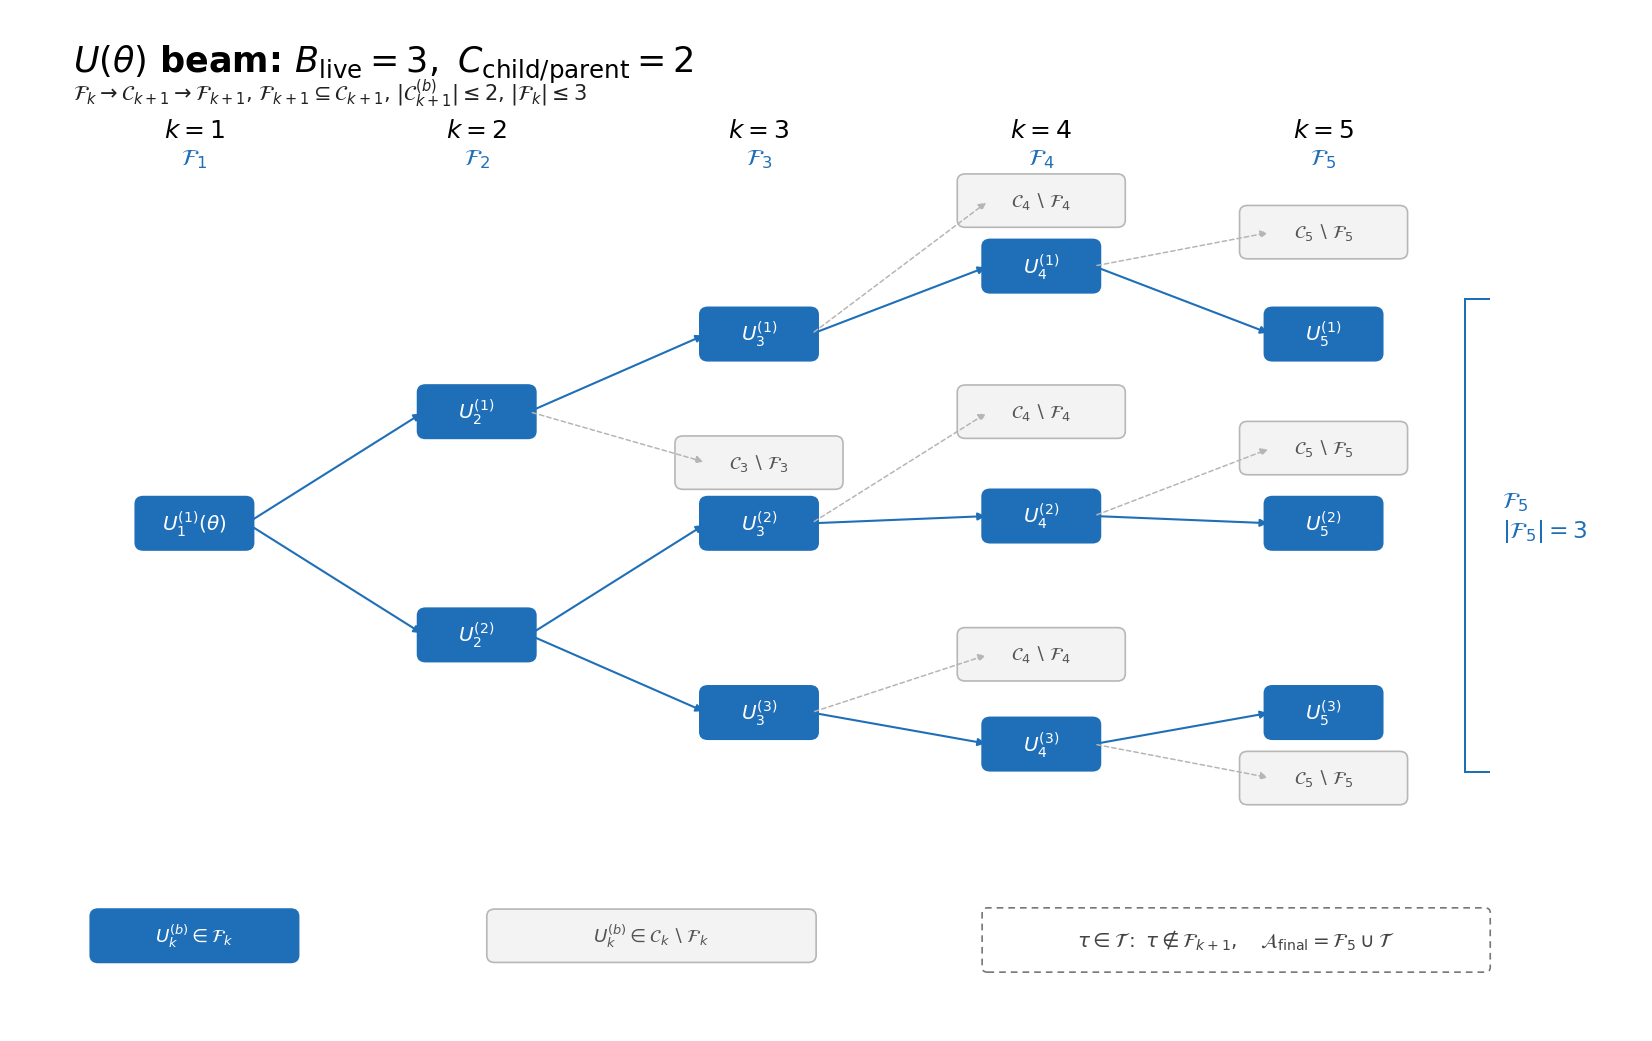
\includegraphics[width=\textwidth]{figures/paper_i_beam_tree_example.png}
\caption{Beam-frontier schematic for \(B_{\mathrm{live}}=3\) and \(C_{\mathrm{child/parent}}=2\).  The update is \(\mathcal F_k\to\mathcal C_{k+1}\to\mathcal F_{k+1}\), with \(\mathcal F_{k+1}\subseteq\mathcal C_{k+1}\), blue nodes \(U_k^{(b)}\in\mathcal F_k\), grey nodes \(U_k^{(b)}\in\mathcal C_k\setminus\mathcal F_k\), and terminal snapshots \(\tau\in\mathcal T\) entering only \(\mathcal A_{\mathrm{final}}=\mathcal F_5\cup\mathcal T\).}
\label{fig:beam_tree_example}
\end{figure*}









\section{Controller useful runway}
\label{app:controller_useful_runway}

% Historical compact forecaster block retained for comparison with the
% implementation-facing live-prune controller in Appendix~\ref{app:prune}.
With \(D_{\rm left}(t)\) remaining admissions and a plateau/degeneracy hazard \(h_t(q)\), the ansatz-extension forecast is
\begin{equation}
\begin{aligned}
\widehat N_{\rm rem}(t)
={}&
\sum_{q=1}^{D_{\rm left}(t)}
\left[\prod_{j=1}^{q-1}(1-h_t(j))\right]
\\
&\quad\times
\Phi\!\left(\frac{m_t-\gamma_t(q-1)-u_t}{s_t}\right),
\\
R_t&=\frac{\widehat N_{\rm rem}(t)}{D_{\rm left}(t)+\eps} .
\end{aligned}
\label{eq:expected_utility_left_archival}
\end{equation}
Here \(D_{\rm left}(t)\) is the remaining admission budget, \(h_t(q)\) is the probability of losing the \(q\)-th future admission to plateau or degeneracy, \(\Phi\) is the standard normal cumulative distribution function, \(m_t\) and \(s_t\) are the running location and scale of the admitted progress statistic \(Z_s\), \(\gamma_t(q-1)\) is the forecasted decay of marginal utility after \(q-1\) further admissions, \(u_t\) is the minimum useful-progress threshold, and \(\eps\) prevents division by zero. Large \(R_t\) indicates that useful admissions remain; small \(R_t\) contracts insertion-position breadth, inherited refit breadth, shortlist breadth, and expensive phase usage.


\section{Generator ablation and useful-runway control}
\label{app:generator_ablation_useful_runway_control}

At accepted adaptive step \(k\), after candidate admission and refit, write the live child branch as
\[
\begin{aligned}
\Xi_k^+
&:=
\bigl(\mathcal O_k^+,\boldsymbol\theta_k^+,E_k^+\bigr),
\\
\mathcal O_k^+
&:=(d_1,\ldots,d_{n_k}),
\\
U(\mathcal O_k^+,\boldsymbol\theta_k^+)
&:=
\prod_{r=n_k}^{1}
\exp(\theta_{k,r}^+d_r),
\\
E(\mathcal O,\boldsymbol\theta)
&:=
\langle\psi_{\rm ref}|
U^\dagger(\mathcal O,\boldsymbol\theta)H
U(\mathcal O,\boldsymbol\theta)
|\psi_{\rm ref}\rangle .
\end{aligned}
\]
Each active generator coordinate \(d_j\) carries an admission step \(a_j\) and cooldown \(c_j(k)\).  The raw deletion-eligible set is
\[
\mathcal E_k^\ominus
:=
\left\{
j\in\{1,\ldots,n_k\}:
k-a_j\ge p_{\rm protect},\;
c_j(k)\le 0
\right\}.
\]

The live-prune controller is driven by the recent admission-gain history.  For a prior accepted admission \(i<k\),
\[
\begin{aligned}
\delta_i
&:=[E_i^- - E_i^+]_+,
\\
z_i
&:=\operatorname{asinh}\!\left(\frac{\delta_i}{\tau_\delta}\right),
\\
u_\star
&:=
\operatorname{asinh}\!\left(
\frac{\max\{\tau_{\rm weak},\epsilon\}}{\tau_\delta}
\right).
\end{aligned}
\]
At step \(k\),
\[
\begin{aligned}
m_k&:=\operatorname{EWMA}_\alpha(z_0,\ldots,z_{k-1}),
\\
s_k&:=\max\{s_{\min},\operatorname{MAD}(z_0,\ldots,z_{k-1})\},
\\
D_k&:=(K_{\max}-k)_+ .
\end{aligned}
\]
Define the local plateau and low-gain streak counts by
\[
\begin{aligned}
C_k^{\rm plat}
&:=
\max\left\{
h\le W_k^{\rm plat}:
z_{k-r}\le u_k^{\rm plat}
\; \text{for all}\; r=1,\ldots,h
\right\},
\\
C_k^{\rm low}
&:=
\max\left\{
h\le W_k^{\rm low}:
z_{k-r}\le u_\star
\; \text{for all}\; r=1,\ldots,h
\right\},
\\
u_k^{\rm plat}
&:=
\left(
\eta_0+\eta_1\left[1-\frac{D_k}{K_{\max}}\right]
\right)m_k .
\end{aligned}
\]
With \(\Pi_{[0,1]}(x):=\min\{1,\max\{0,x\}\}\), the stagnation pressure is
\[
u_k^{\rm stag}
:=
\Pi_{[0,1]}
\max\left\{
\frac{C_k^{\rm plat}}{W_k^{\rm plat}},
\frac{C_k^{\rm low}}{W_k^{\rm low}}
\right\}.
\]
Let \(R_k^{\rm rec}\) and \(R_k^{\rm old}\) denote recent and older EWMA admission gains.  Set
\[
\begin{aligned}
\rho_k
&:=
\max\left\{
\rho_{\min},
\min\left[
1,\frac{R_k^{\rm rec}}{\max\{R_k^{\rm old},\epsilon\}}
\right]
\right\},
\\
\gamma_k
&:=
-\log\bigl(\max\{\rho_k,\epsilon\}\bigr).
\end{aligned}
\]
For future admission offset \(q=1,\ldots,D_k\), define
\[
\begin{aligned}
p_{kq}^{\rm use}
&:=
\Phi\!\left(
\frac{m_k-\gamma_k(q-1)-u_\star}
{\max\{s_k,s_{\min}\}}
\right),
\\
h_{kq}
&:=
\sigma\!\left(
\beta_0+\beta_{\rm stag}u_k^{\rm stag}
+\beta_{\rm front}\varphi_k
+\eta_h(q-1)
\right),
\\
S_{k1}&:=1,\qquad
S_{kq}:=\prod_{r=1}^{q-1}(1-h_{kr})\quad(q\ge2),
\end{aligned}
\]
where \(\varphi_k\in[0,1]\) is frontier/beam pressure, \(h_{kq}\) is the forecast hazard that useful extension terminates before offset \(q\), and \(S_{kq}\) is the corresponding survival factor.  The predicted number of useful remaining admissions is
\[
\widehat N_{\rm rem}(k)
:=
\min\left\{
D_k,\,
\left[
\sum_{q=1}^{D_k}S_{kq}p_{kq}^{\rm use}
\right]_+
\right\}.
\]
The prune-maturity controller term is therefore
\[
\Omega_k^{\rm NREM}
:=
1-
\Pi_{[0,1]}
\left(
\frac{\widehat N_{\rm rem}(k)}
{D_k+\epsilon}
\right).
\]
Thus \(\Omega_k^{\rm NREM}\approx0\) when useful adaptive runway remains, and \(\Omega_k^{\rm NREM}\approx1\) when the branch is forecast to be near saturation.  Live pruning is permitted only when
\[
\Gamma_{k,{\rm live}}^\ominus
:=
M_{\rm live}\,
\mathbf 1\{n_k>1\}\,
\mathbf 1\{S_k^{\rm refit}=1\}\,
\mathbf 1\{A_k^{\rm adm}=1\}\,
\mathbf 1\{\Omega_k^{\rm NREM}\ge u_{\min}\}
=1 .
\]
The live deletion-candidate set is
\[
\mathcal C_k^\ominus
:=
\left\{
j\in\mathcal E_k^\ominus:
\Gamma_{k,{\rm live}}^\ominus=1
\right\}.
\]

For \(j\in\mathcal C_k^\ominus\), let \(\bar{\jmath}:=\{1,\ldots,n_k\}\setminus\{j\}\).  SNAKE tests whether the surviving coordinates can locally recover the deleted generator through a nested survivor-window ladder
\[
\varnothing=W_{j,0}
\subseteq W_{j,1}
\subseteq\cdots
\subseteq W_{j,S_j}
\subseteq\bar{\jmath}.
\]
At \(\boldsymbol\theta_k^+\), define
\[
\begin{aligned}
g_j&:=\partial_{\theta_j}E(\mathcal O_k^+,\boldsymbol\theta_k^+),
\\
h_j&:=\partial_{\theta_j}^2E(\mathcal O_k^+,\boldsymbol\theta_k^+),
\\
b_{j,s}
&:=
\left(
\partial_{\theta_i}\partial_{\theta_j}E
\right)_{i\in W_{j,s}},
\\
H_{j,s}
&:=
\left(
\partial_{\theta_i}\partial_{\theta_\ell}E
\right)_{i,\ell\in W_{j,s}},
\\
R_{j,s}
&:=
\frac12(H_{j,s}+H_{j,s}^{\top})+\lambda_H I .
\end{aligned}
\]
Deleting \(d_j\) corresponds to the coordinate displacement
\[
\alpha_j=-\theta_{k,j}^+ .
\]
The Schur-relaxed survivor response is
\[
\delta\boldsymbol\theta_{W_{j,s}}^\star
=
-\alpha_jR_{j,s}^{-1}b_{j,s}
=
\theta_{k,j}^+R_{j,s}^{-1}b_{j,s}.
\]
Substitution into the local quadratic model gives the rungwise deletion-loss surrogate
\[
\begin{aligned}
\Lambda_{j,s}^{\ominus}
&:=
g_j\alpha_j
+\frac12\alpha_j^2
\left(
h_j-b_{j,s}^{\top}R_{j,s}^{-1}b_{j,s}
\right)
\\
&=
-g_j\theta_{k,j}^+
+\frac12(\theta_{k,j}^+)^2
\left(
h_j-b_{j,s}^{\top}R_{j,s}^{-1}b_{j,s}
\right).
\end{aligned}
\]
For \(W_{j,0}=\varnothing\), the Schur term is defined as \(b_{j,0}^{\top}R_{j,0}^{-1}b_{j,0}=0\).  The first surrogate-passing rung is
\[
s_j^\star
:=
\min\left\{
s:
\Lambda_{j,s}^{\ominus}
\le \varepsilon_{k,{\rm schur}}^\ominus
\right\},
\]
with \(s_j^\star=\infty\) if no rung passes.  The Schur-screened nomination set is
\[
\mathcal N_k^\ominus
:=
\operatorname{Top}_{M_{\max}}
\operatorname{sort}_{\Lambda}
\left\{
j\in\mathcal C_k^\ominus:
s_j^\star<\infty
\right\}.
\]
The measured delete-refit branch for \(j\in\mathcal N_k^\ominus\) is
\[
\begin{aligned}
\mathcal O_{k,-j}^{(s_j^\star)}
&:=
\mathcal O_k^+\ominus d_j,
\\
\boldsymbol\theta_{k,-j}^{(s_j^\star)}
&:=
\argminp_{\boldsymbol\vartheta}
E(\mathcal O_{k,-j}^{(s_j^\star)},\boldsymbol\vartheta),
\\
\operatorname{supp}
\left(
\boldsymbol\vartheta-\boldsymbol\theta_{k,\bar{\jmath}}^+
\right)
&\subseteq W_{j,s_j^\star},
\\
E_{k,-j}^{(s_j^\star)}
&:=
E(\mathcal O_{k,-j}^{(s_j^\star)},\boldsymbol\theta_{k,-j}^{(s_j^\star)}).
\end{aligned}
\]
Equivalently, for the frozen-delete specialization used when no survivor refit is opened,
\[
\begin{aligned}
W_{j,0}&=\varnothing,
\\
\boldsymbol\theta_{k,-j}^{[0]}
&=(\theta_{k,i}^+)_{i\ne j},
\\
\Delta E_j^{\ominus,[0]}
&=
E(\mathcal O_k^+\ominus d_j,\boldsymbol\theta_{k,-j}^{[0]})
-
E(\mathcal O_k^+,\boldsymbol\theta_k^+)
\\
&=
\sum_\ell h_\ell
\left(
\langle P_\ell\rangle_{k,-j,[0]}
-
\langle P_\ell\rangle_{k,+}
\right),
\end{aligned}
\]
where \(H=\sum_\ell h_\ell P_\ell\).  In the general rung case,
\[
\Delta E_j^{\ominus}
:=
E_{k,-j}^{(s_j^\star)}-E_k^+ .
\]
The deletion tolerance is scaled to recent useful progress,
\[
\begin{aligned}
\Delta_{{\rm scr},k}
&:=
\max\left\{
\tau_{\rm weak},
\operatorname{EWMA}_{1/2}(\delta_{k-r},\ldots,\delta_{k-1}),
\epsilon_{\rm mach},
\epsilon_{\rm abs}
\right\},
\\
\varepsilon_k^\ominus
&:=
\max\left\{
\epsilon_{\rm abs},
\xi_\ominus\Delta_{{\rm scr},k}
\right\}.
\end{aligned}
\]
Let
\[
\begin{aligned}
G_k^{\rm adm}
&:=[E_k^- - E_k^+]_+,
\\
G_j^{\rm ret}
&:=E_k^- - E_{k,-j}^{(s_j^\star)} .
\end{aligned}
\]
The measured accept/reject variable is
\[
A_j^\ominus
:=
\mathbf 1\{\Delta E_j^\ominus\le \varepsilon_k^\ominus\}
\mathbf 1\{G_j^{\rm ret}\ge \rho_{\rm ret}G_k^{\rm adm}\}
\mathbf 1\{C_j^{\rm curv}=1\}.
\]
The committed branch update is
\[
\Xi_k^{\rm out}
=
\begin{cases}
\bigl(
\mathcal O_k^+\ominus d_j,
\boldsymbol\theta_{k,-j}^{(s_j^\star)},
E_{k,-j}^{(s_j^\star)}
\bigr),
& A_j^\ominus=1,
\\[2mm]
\bigl(
\mathcal O_k^+,
\boldsymbol\theta_k^+,
E_k^+
\bigr),
& A_j^\ominus=0 .
\end{cases}
\]
On rejection, only the deletion trial is discarded:
\[
A_j^\ominus=0
\quad\Longrightarrow\quad
c_j(k+1)=c_{\rm cool},
\qquad
\Xi_k^{\rm out}=\Xi_k^+ .
\]
Thus prune rollback is local to the post-admission child branch, not to the pre-admission parent branch.  On acceptance, \(d_j\) is removed from the live ansatz and the reduced child branch enters the beam frontier for step \(k+1\).

For the Hubbard--Holstein runs, the live-prune constants used in this appendix were
\[
\begin{gathered}
K_{\max}=30,\qquad
p_{\rm protect}=2,\qquad
c_{\rm cool}=2,\qquad
M_{\max}=6,\qquad
\rho_{\rm ret}=\frac12,
\\
\tau_\delta=10^{-6},\qquad
\tau_{\rm weak}=10^{-9},\qquad
\epsilon=10^{-12},\qquad
\epsilon_{\rm mach}=10^{-12},\qquad
\epsilon_{\rm abs}=10^{-8},
\\
\xi_\ominus=0.01,\qquad
\alpha=0.4,\qquad
s_{\min}=10^{-3},\qquad
\rho_{\min}=0.25,\qquad
u_{\min}=0.5 .
\end{gathered}
\]
The controller coefficients \(\beta_0,\beta_{\rm stag},\beta_{\rm front},\eta_h,\eta_0,\eta_1\), the EWMA windows, and the precise survivor-window construction are recorded in the reproducibility metadata for the displayed rows rather than expanded further here.

\fi

\section{Hubbard control benchmarks}

For the Hubbard chain, the weak-coupling limit is given by
\(U/t\ll 1\), with correlation strength increasing as \(U/t\) grows;
we use \(U/t=0.25\) as a weak regime representative and \(U/t=8\) as the strong-correlation point
\cite{Arovas2022Hubbard}.  

We find that all methods converge easily in the Hubbard $L=2$ strong-regime, whereas first-order gradient-based methods plateau in the weak-regime due to repeated selections of single unitary coupled cluster generators, when a double is required. 

% Machine provenance: native main Table I rows refreshed on 2026-05-25
% from the partial CHTC v3/v4 three-model update archive:
% tmp/chtc_partial_paper_i_three_model_v3_v4_20260525/extracted.
% Comparator rows are from cluster 6945817, and SNAKE rows are from
% cluster 6945865.
% SNAKE rows are Optuna jobs; the displayed completed SNAKE cells use the
% selected best trial in each finished job, not an arbitrary trial.
% Resource cells use Qiskit-compiled displayed-ansatz costs: below-threshold
% adaptive prefix when present and final terminal ansatz otherwise.
% Fidelity cells are post-hoc reporting metrics from the same enrichment path;
% -- means the displayed source row is running, skipped, or unreconstructible.
% Support maps are regenerated by
% pipelines/reporting/build_paper_i_three_model_support_maps.py, which merges
% comparator enrichment sidecars with completed Route-A/SNAKE Optuna summaries.
% Terminal non-hit comparator costs are sourced from:
% output/pdf/paper_i_three_model_terminal_cost_recovery_20260525.json
% Hubbard depth-500 repair cells promoted from:
% output/pdf/paper_i_hubbard_depth500_repair_table_update_20260525.json
% Repair cluster 6946127 completed Pos-Geo, Qubit/QEB, append-strong, and
% TETRIS-weak rows; append-weak and TETRIS-strong were running in that snapshot.
% Running or incomplete replacement evidence must not erase prior displayed table
% data unless the user explicitly approves that destructive replacement.
% promoted sidecars:
% raw_outputs/paper_i_three_model_metric_enrichment_selected_logical_20260525_v1
% raw_outputs/paper_i_three_model_metric_enrichment_selected_logical_20260525_v2
% output/pdf/paper_i_three_model_fidelity_sources_20260525.json
% and completed CHTC v2 comparator rows fetched under:
% tmp/paper_i_three_model_comparators_v2_jsons_20260525/raw_outputs.
% Current partial update support:
% output/pdf/paper_i_three_model_partial_chtc_v3_v4_table_update_20260525.json
% output/pdf/paper_i_hubbard_table_i_prefix_fidelity_update_20260526.json
% Keep these paths in comments only; do not render them in the manuscript.
% BEGIN_TABLE_I_II_DEPTH_PROVENANCE_HYGIENE_20260609
% Tables I--II depth convention: fixed-structure rows have no ADAPT depth.
% Adaptive rows use terminal/reported source depths from
% MATH/paper_facing/paper_I_static_scaffold/paper_i_tables_i_ii_spsa_optuna_current_best_promotion_20260601.json
% unless output/pdf/paper_i_tables_i_ii_visible_prefix_cost_audit_20260528.json
% overrides the displayed resource prefix.
% Active adaptive comparator depths are now from the 2026-06-10 repeat-enabled fixed-horizon Suite B source.
% Hubbard append 80/20, native full-meta TETRIS 106/23, Geo 80/20, Qubit/QEB 80/20 selected operators.
% Spin-boson append 20/20, TETRIS 32/41, Geo 20/20, Qubit/QEB 20/20 selected operators.
% SNAKE final operator counts remain row-specific provenance: Hubbard weak/strong 3/3;
% spin-boson weak/strong 4/8 from the joint batch-2 source.
% END_TABLE_I_II_DEPTH_PROVENANCE_HYGIENE_20260609
% BEGIN_MACHINE_READABLE_TABLE_I_II_DATA_ANALYSIS_CONTINUATION_REPORT_20260609
% {"schema":"paper_i_tables_i_ii_data_analysis_continuation_report_v1","updated_date":"2026-06-09","scope":"hidden provenance for standalone diagnostic PDF/JSON only; no manuscript-visible table/prose changes","report_pdf":"output/pdf/paper_i_data_analysis_hubbard_spinboson_iteration_plateau_20260609.pdf","report_pdf_sha256":"5c2d1a95c6ed44dd8f293067137e58a7249bb6b8ebf8722add13c3b8eceadf41","report_json":"output/pdf/paper_i_data_analysis_hubbard_spinboson_iteration_plateau_20260609.json","report_json_sha256":"66c309203a9aeaaa1cefcd0e56ac0712f0024175371e1a658f770f0e3ddb12d9","continuation_summary":"tmp/paper_i_hubbard_spin_boson_local_continuations_20260609_v2/summary.json","continuation_summary_sha256":"b9af2002fe1caffb2146562827ff0cd961d151f9651344c97384466a7a5016b9","source_locked_snake_manifest":"tmp/paper_i_snake_source_locked_continuations_20260609_v2/manifest.json","source_locked_snake_manifest_sha256":"f3faf227b1243c0f70a828972c5dd4ad7c48a54ca1724a123ce89f7be2e79fd2","append_only_extension_manifest":"tmp/paper_i_append_only_extensions_20260609_v1/manifest.json","append_only_extension_manifest_sha256":"8a12e01f89a8b25b2196cadeaaee2f89c0357da61029ecffdd7c377b9a98be9d","valid_rows":20,"retained_snake_source_rows":2,"source_locked_spin_boson_snake_rows":2,"append_extension_rows":2,"quarantined_rows":2,"caps":{"hubbard_weak":80,"hubbard_strong_append_observed_terminal":18,"spin_boson_weak_append_observed_terminal":44,"spin_boson_strong":20},"policy":"diagnostic local continuations only; no CHTC; four report tables; plot x-axes use integer accepted-prefix ticks; dashed terminal holds are display-only and do not add cost; spin-boson SNAKE rows use direct source-locked no-target continuations through depth 20; spin-boson weak Append and Hubbard strong Append use append-only extension records through pool exhaustion; earlier generic Phase3 spin-boson SNAKE attempts remain quarantined"}
% END_MACHINE_READABLE_TABLE_I_II_DATA_ANALYSIS_CONTINUATION_REPORT_20260609
% BEGIN_MACHINE_READABLE_TABLE_I_II_RAW_ERROR_REDISPLAY_20260609
% {"schema":"paper_i_tables_i_ii_raw_absolute_error_redisplay_v2","updated_date":"2026-06-10","scope":"visible Tables I-II error columns after repeat-enabled adaptive comparator update; fixed HEA/family rows retained; SNAKE rows from joint batch-2 source","display_error_policy":"raw absolute energy error |E_alg-E_ref| at the displayed ansatz/prefix","target_role":"E_T=2e-4 retained as useful convergence target for table interpretation; target guide lines are not rendered in iteration plots; errors are not target-subtracted","source":"MATH/paper_facing/paper_I_static_scaffold/paper_i_tables_i_ii_repeat_enabled_comparator_promotion_20260610.json plus output/pdf/paper_i_joint_batch2_cost_search_promotion_20260610.json","hubbard_raw_errors":{"HEA":["3.10e-8","5.86e-8"],"family":["2.81e-8","5.92e-8"],"append":["1.56e-2","8.69e-5"],"TETRIS":["1.55e-2","1.36e-1"],"Geo":["3.15e-4","5.23e-6"],"Qubit/QEB":["1.82e-4","2.14e-7"],"SNAKE":["6.66e-16","1.33e-14"]},"spin_boson_display_error_policy":"same-cutoff ED at n_ph_work; higher-cutoff external errors diagnostic only","spin_boson_raw_errors":{"HEA":["3.05e-8","4.87e-3"],"family":["1.67e-3","6.70e-3"],"append":["6.16e-7","1.04e-5"],"TETRIS":["6.16e-7","1.09e-5"],"Geo":["6.16e-7","9.97e-6"],"Qubit/QEB":["1.67e-3","6.70e-3"],"SNAKE":["6.16e-7","9.97e-6"]}}
% END_MACHINE_READABLE_TABLE_I_II_RAW_ERROR_REDISPLAY_20260609
% BEGIN_MACHINE_READABLE_TABLE_I_II_JOINT_BATCH2_SNAKE_PROMOTION_20260610
% {"schema":"paper_i_tables_i_ii_joint_batch2_snake_promotion_pointer_v1","updated_date":"2026-06-10","scope":"condensed manuscript benchmark paragraph and visible appendix SNAKE rows updated from user-approved joint Hubbard/spin-boson batch-2 hard-gate evidence","summary_json":"output/pdf/paper_i_joint_batch2_cost_search_promotion_20260610.json","summary_sha256":"e8e5f12ebebf15187dffb51e212fec6d53e96f9920d887c943129dbb2b4521f8","analysis_pdf":"output/pdf/paper_i_data_analysis_hubbard_spinboson_iteration_plateau_20260609.pdf","analysis_pdf_sha256":"5c2d1a95c6ed44dd8f293067137e58a7249bb6b8ebf8722add13c3b8eceadf41","frozen_trial":3,"policy":"same shared batched SNAKE settings across Hubbard weak/strong and spin-boson weak/strong; Table II spin-boson errors displayed as same-cutoff ED at n_ph_work with higher-ED external errors retained as diagnostics; target-hit stop disabled; terminal compiled costs reported where per-prefix compile sidecars are unavailable; earlier repeated-double Hubbard diagnostic not used for table-facing costs"}
% END_MACHINE_READABLE_TABLE_I_II_JOINT_BATCH2_SNAKE_PROMOTION_20260610
% BEGIN_MACHINE_READABLE_TABLES_I_II_FINAL_COST_DISPLAY_UPDATE_20260619
% {"schema":"paper_i_tables_i_ii_final_cost_display_update_v1","updated_date":"2026-06-19","scope":"visible Hubbard and spin-boson/Rabi cost cells","policy":"display final reported plateau/terminal cost cells for adaptive comparators; first-threshold-hit TETRIS spin-boson costs are retired from the rendered tables","tetris_terminal_source":"output/pdf/paper_i_data_analysis_hubbard_spinboson_iteration_plateau_20260609.json","tetris_spin_boson_cells":{"weak":{"DeltaE":"6.16e-7","N2q":119,"D2q":107,"Dc":750,"S":173390},"strong":{"DeltaE":"9.97e-6","N2q":711,"D2q":623,"Dc":3544,"S":5823}},"snake_s_source":"MATH/paper_facing/paper_I_static_scaffold/paper_i_tables_i_ii_repeat_enabled_comparator_promotion_20260610.json","snake_s_cells":{"hubbard_weak":21919,"hubbard_strong":21919,"spin_boson_weak":30043,"spin_boson_strong":38440},"display_policy":"visible S cells use ordinary decimal numerals and the column label S, not S_alg or legacy controller_shot_proxy"}
% END_MACHINE_READABLE_TABLES_I_II_FINAL_COST_DISPLAY_UPDATE_20260619
% BEGIN_MACHINE_READABLE_TABLE_I_HUBBARD_U8_STRONG_UPDATE_20260614
% {"schema":"paper_i_hubbard_u8_strong_update_v2","updated_date":"2026-06-14","table_label":"tab:fixed_accuracy_claims","main_figure_label":"fig:hubbard_weak_iteration_trace","main_plot_pdf":"output/pdf/paper_i_data_analysis_hubbard_weak_repeat_enabled_error_vs_iteration_20260610.pdf","appendix_strong_figure_label":"fig:appendix_hubbard_strong_iteration_trace","appendix_strong_plot_pdf":"output/pdf/paper_i_true_strong_replacement_20260613_hubbard_u8_strong.pdf","source_report":"output/pdf/paper_i_true_strong_replacement_20260613.json","source_report_sha256":"72050c03ef1ada9a86b151acb7a66ac1fa269935be272ba3f3328af85a281b07","source_tex":"output/pdf/paper_i_true_strong_replacement_20260613.tex","source_tex_sha256":"678fa34c284f553a0a3b5b4c2584fd848bd10c84464739781e036b23eb66f996","metric_policy":"raw exact-diagonalization energy error for Hubbard rows; U/t=8 for the strong table and appendix strong plot","display_note":"Hubbard weak and strong convergence plots swapped on 2026-06-14: weak trace is now the main text Hubbard figure; U/t=8 strong trace is retained in the supplementary Hubbard block. Hubbard--Holstein U/t=8 full-comparator replacement remains incomplete because CHTC 7651653 procs 2,8,9,10 were still running at retrieval time"}
% END_MACHINE_READABLE_TABLE_I_HUBBARD_U8_STRONG_UPDATE_20260614
% BEGIN_MACHINE_READABLE_PAPER_I_LOCAL_PROVENANCE_AUDIT_20260621
% {"schema":"paper_i_local_provenance_audit_pointer_v1","updated_date":"2026-06-21","support_json":"MATH/paper_facing/paper_I_static_scaffold/paper_i_local_provenance_audit_20260621.json","scope":"local provenance audit for current Paper-I data pointers and weak-Hubbard SPSA/SNAKE ablation claim","status":"HH native200 local complete; weak-Hubbard ablation local complete; older Tables I-II row-level sources not fully local"}
% END_MACHINE_READABLE_PAPER_I_LOCAL_PROVENANCE_AUDIT_20260621
% BEGIN_MACHINE_READABLE_PAPER_I_HUBBARD_WEAK_PREFIX30_UPDATE_20260621
% {"schema":"paper_i_hubbard_weak_prefix30_append_geo_snake_update_pointer_v1","updated_date":"2026-06-21","support_json":"MATH/paper_facing/paper_I_static_scaffold/paper_i_hubbard_weak_u025_prefix30_append_geo_snake_update_20260621.json","support_json_sha256":"ddafa90f49aff8bee886e163bcc83a05c7295b7b211f586426fdf367d5dc5936","scope":"visible weak-Hubbard U/t=0.25 main iteration plot and appendix Qiskit cost table for Append, Geo, and SNAKE","display_policy":"30-iteration prefix; S reconstructed through the same prefix from per-iteration optimizer and controller/probe work"}
% END_MACHINE_READABLE_PAPER_I_HUBBARD_WEAK_PREFIX30_UPDATE_20260621
% BEGIN_PLACEHOLDER_WEAK_HUBBARD_DUAL_PLOTS_20260626
% Keep both temporarily. Legacy diagnostic plot supports early-SNAKE/long-Geo prose.
% Current U/t=0.25 plot supports the active 30-prefix run. Delete one after choosing.
% Legacy plot source: output/pdf/paper_i_data_analysis_hubbard_weak_error_vs_iteration_20260610.png sha256=416d54fbae17e2bbecc6dd72b27ed49a56a5bf3bcd188170ac436458ed048647.
% Current plot source: MATH/paper_details/figures/paper_i_hubbard_weak_u0p25_append_geo_snake_overlay_20260621.png sha256=e5c377e69fc3bf9dc0e46919348cd92d0ceb261494056db766ac4f7d050dae86.
\noindent\begin{minipage}{\columnwidth}
\centering
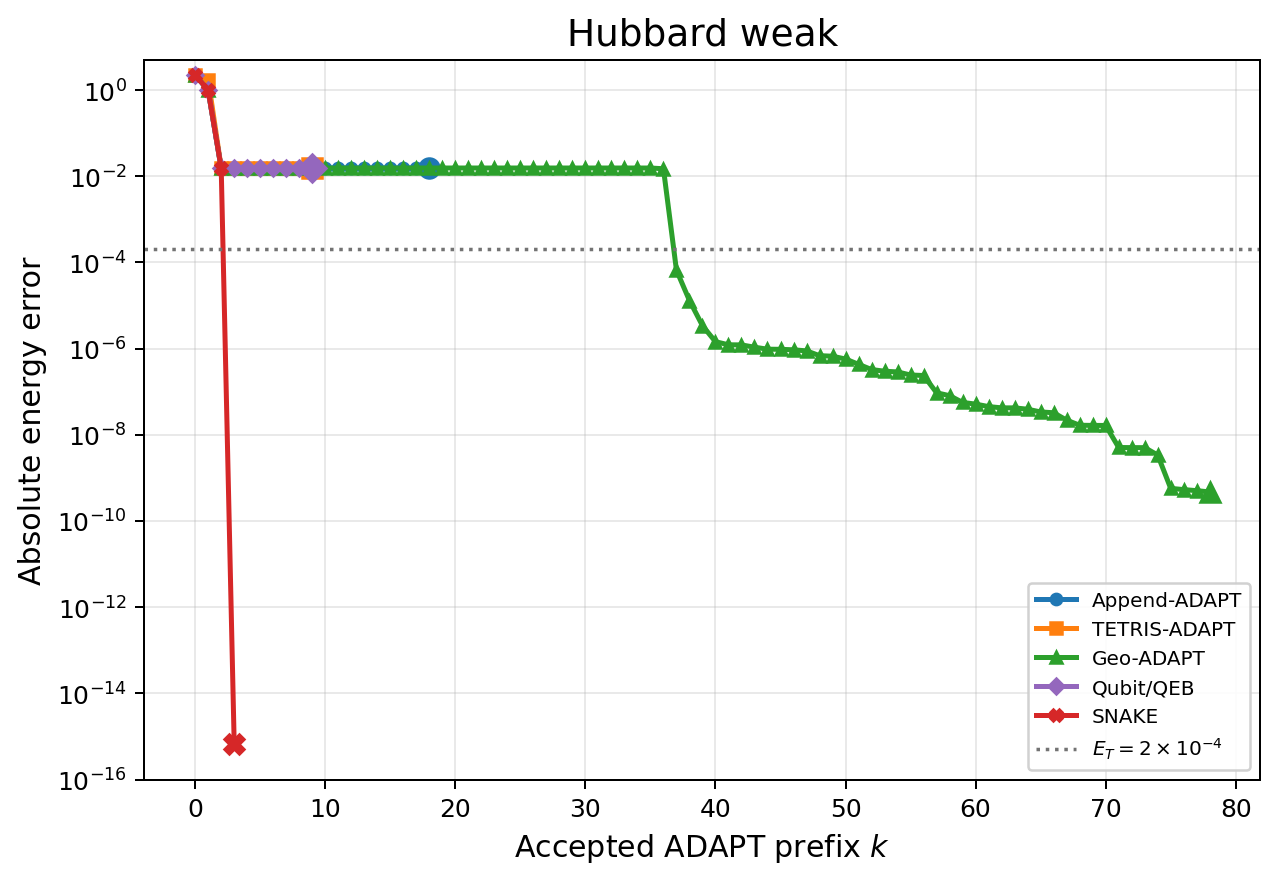
\includegraphics[width=\columnwidth]{figures/paper_i_hubbard_weak_supportive_diagnostic_20260610.png}
\captionof{figure}{Legacy weak-Hubbard diagnostic convergence trace, plotted as absolute same-cutoff energy error versus ADAPT selection iteration.}
\label{fig:hubbard_weak_iteration_trace_support_legacy}
\end{minipage}
\par\addvspace{0.8ex}
% END_PLACEHOLDER_WEAK_HUBBARD_DUAL_PLOTS_20260626
\noindent\begin{minipage}{\columnwidth}
\centering
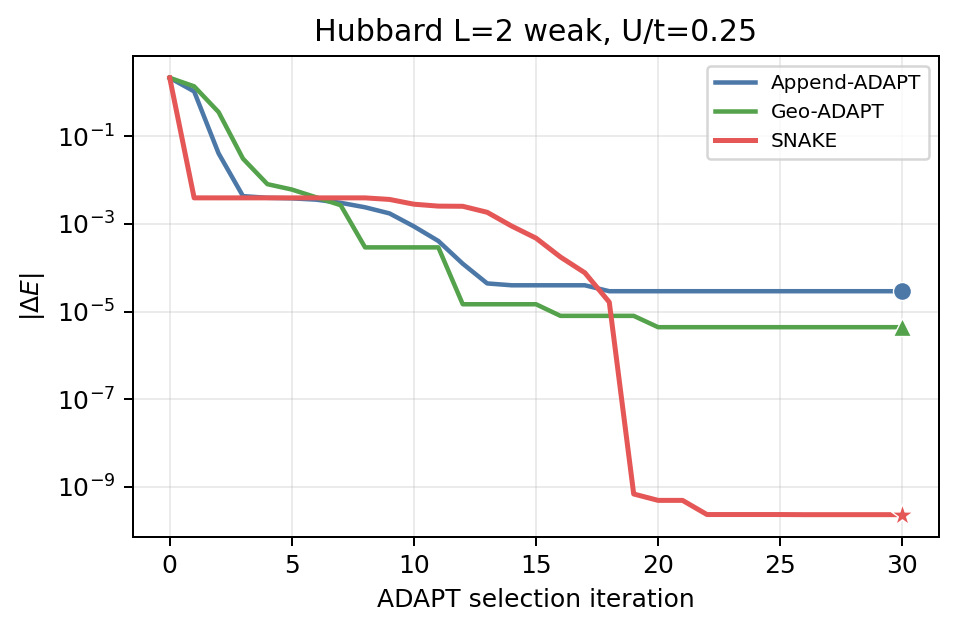
\includegraphics[width=\columnwidth]{figures/paper_i_hubbard_weak_u0p25_append_geo_snake_overlay_20260621.png}
\captionof{figure}{Weak-Hubbard convergence trace at \(U/t=0.25\), plotted as absolute same-cutoff energy error versus ADAPT selection iteration.}
\label{fig:hubbard_weak_iteration_trace}
\end{minipage}
\par\addvspace{0.8ex}

Displayed weak-Hubbard traces at \(U/t=0.25\) show Append-ADAPT and Geo-ADAPT stagnating on repeated UCC single selections over the 30-iteration window, while SNAKE admits the two spin-resolved singles followed by a UCC double and reaches \(|\Delta E|=2.34\times10^{-10}\).
In the strong-Hubbard dimer at \(U/t=8\), all methods converge within a few accepted generators.
Weak-Hubbard ablations isolate the recovery mechanism: phase-I-only scoring remains plateaued, second-order Fubini--Study scoring without tangent novelty reaches \(2.8\times10^{-6}\) error by iteration 9 at SPSA budget 1000, and tangent novelty without the second-order score reaches \(1.7\times10^{-6}\) by iteration 8 and \(5.1\times10^{-7}\) by iteration 9 at SPSA budget 8000.
Geo-ADAPT reaches \(4.72\times10^{-10}\) only after raising the SPSA budget to 8000 and continuing to iteration 78, while Append-ADAPT reaches the \(10^{-8}\)-scale at iteration 13 under the same SPSA budget but remains above \(10^{-8}\) through iteration 100; these diagnostics lie outside the displayed 30-iteration comparison, so the weak-regime failure is budget- and scoring-dependent rather than an operator-pool impossibility.
This also explains the lower estimator-work proxy relative to Geo-ADAPT: SNAKE applies full-pool gradient screening before Fubini--Study tangent probes, avoiding the full-pool \(O(n^2)\) Gram-matrix measurement burden.


\section{Operator pools used for Hubbard and Hubbard--Holstein}
\label{app:pools}

We define the pre-encoding operator pool as \(\Gset=\{G_\nu\}\), where
\(G_\nu\) is a fermionic, bosonic, or mixed second-quantized generator.  After
Jordan--Wigner fermion mapping and binary bosonic encoding with register
truncation, \(G_\nu\) is represented by an encoded Hermitian Pauli polynomial
\(\widehat G_\nu\), and the implemented ansatz layer is
\(\exp(-\ii\theta_\nu\widehat G_\nu)\).

For the Hubbard--Holstein phonon registers, \(b_i^\dagger,b_i\) create and annihilate a truncated
oscillator quantum on site or mode \(i\).  The bosonic operator pool uses
quadrature and transport channels because the oscillator must respond by
displacement, conjugate motion, occupation change, width change, and
cutoff-sensitive nonlinear response
\cite{Sawaya2020,Li2023,Dutta2024BosonicChemistry,Peng2025BosonHamiltonians}.
We use \(X_i=b_i+b_i^\dagger\), \(P_i=\ii(b_i^\dagger-b_i)\),
\(n_{b,i}=b_i^\dagger b_i\), \(S_i=\ii[(b_i^\dagger)^2-b_i^2]\),
and include \(X_i\), \(P_i\), \(n_{b,i}\), \(S_i\), \(X_i^2\), \(P_i^2\),
\(n_{b,i}^2\), \(X_iP_i+P_iX_i\), \(X_iX_j\), \(P_iP_j\),
\(b_i^\dagger b_j+b_j^\dagger b_i\),
\(\ii(b_i^\dagger b_j-b_j^\dagger b_i)\), phonon-number-weighted transport,
pair transport, and Kerr \(n_{b,i}(n_{b,i}-I)\).

For the Hubbard--Holstein Hamiltonian, \(n_i\) is the fermionic site-number
operator, \(D_i=n_i-\bar n I\), \(X_i=b_i+b_i^\dagger\),
\(P_i=\ii(b_i^\dagger-b_i)\), \(n_{b,i}=b_i^\dagger b_i\), and
\(S_i=\ii[(b_i^\dagger)^2-b_i^2]\).  The spin-summed hopping and current
operators are \(T_{ij}=\sum_\sigma(c_{i\sigma}^\dagger c_{j\sigma}
+c_{j\sigma}^\dagger c_{i\sigma})\) and
\(J_{ij}=\ii\sum_\sigma(c_{i\sigma}^\dagger c_{j\sigma}
-c_{j\sigma}^\dagger c_{i\sigma})\).  For the fermionic sector, \(i,j\)
denote occupied spin orbitals, \(a,b\) virtual spin orbitals, and
\(\sigma,\sigma'\in\{\uparrow,\downarrow\}\).  The UCCSD single- and
double-excitation generators are
\(G_{i\to a,\sigma}=\ii(c_{a\sigma}^{\dagger}c_{i\sigma}
-c_{i\sigma}^{\dagger}c_{a\sigma})\) and
\(G_{ij\to ab,\sigma\sigma'}=\ii(c_{a\sigma}^{\dagger}
c_{b\sigma'}^{\dagger}c_{j\sigma'}c_{i\sigma}-{\rm h.c.})\).  The mixed pool contains local
polaronic channels \(D_iP_i\) and \(D_iS_i\), nonlocal charge-phonon channels
\(D_iP_j\) and \(D_iX_j\), bond-dressing channels \(T_{ij}(P_i-P_j)\),
\(J_{ij}(P_i-P_j)\), \(T_{ij}(P_i+P_j)\), \(T_{ij}(P_i-P_j)^2\), and
\(J_{ij}(P_i-P_j)^3\), the UCCSD electronic channels tensored with either the phonon identity
or phonon-dressing operators, and Hamiltonian-block/HVA channels.  These
channels encode local Lang--Firsov displacement, density-conditioned phonon
dressing, and bond-conditioned polaron motion
\cite{Holstein1959a,Holstein1959b,Sakkinen2015HolsteinDimer}.

In the weak-Holstein Hubbard--Holstein benchmarks, selected adaptive sequences
include bare electronic channels \(G_{\rm UCCSD}\otimes I_b\) together with
polaronic and phonon-dressed channels such as \(D_iP_i\), \(D_iS_i\),
\(T_{ij}(P_i-P_j)\), \(J_{ij}(P_i-P_j)\), and
\(G_{\rm UCCSD}\otimes\) phonon dressing.  In the strong-Holstein benchmarks,
selected channels shift toward \(G_{\rm UCCSD}\otimes\) phonon dressing,
\(D_iP_i\)-type polaron displacement, and \(S_i\)-type phonon squeeze.

The Hubbard benchmarks reuse these UCCSD channels, augmented by Hubbard
lattice hopping/current, number/interaction, density-assisted hopping/current,
exchange/pair-hop, and Hamiltonian-block/HVA channels.

Append-only ADAPT, Geo-ADAPT, and SNAKE use Hamiltonian-local generator pools
for each benchmark. When a result block uses identical post-filter pool
exposure across methods, that equality is stated explicitly in the corresponding
settings paragraph; otherwise the table text records the route-specific pool
profile and runtime exposure.

\section{Algorithm settings and SPSA sensitivity}
\label{app:results_discussion}

The result tables are noiseless compiled hardware-cost comparisons. This section
records the algorithmic setting and SPSA conventions needed to interpret those tables and
states the metric conventions. Appendix~\ref{app:estimator_work_proxy} gives the
full normalized estimator-work accounting for the \(S\) column.

\subsection{Algorithm settings used in the result tables}

All adaptive result-table rows use the Hamiltonian parameters, cutoff/reference pair,
encoding, and compiled resource target stated in the corresponding table
caption. The common inner-optimizer family for the displayed tables is simultaneous
perturbation stochastic approximation (SPSA), using the shared
\texttt{paper\_i\_main\_tables\_spsa\_v1} schedule recorded in the source
manifests \cite{Spall1992SPSA,Kandala2017}. Within this SPSA schedule family,
non-SNAKE comparator rows use Optuna-selected settings at the granularity of the
displayed benchmark: one calibrated profile per Hubbard or spin--boson/Rabi
Hamiltonian, and one profile per Hubbard--Holstein regime \((U/t,\lambda)\).
SNAKE rows are selected from separate Optuna searches over the same SPSA refit
family together with SNAKE-specific geometry, cost, batching, beam,
capped insertion-position windows, capped reduced-geometry refit windows, and
capped ablation-recoverability windows. This choice matches the adaptive
setting because variational parameters are refit after each accepted generator
while the active dimension grows with iteration. SPSA uses two objective
evaluations per optimizer step, independent of the parameter dimension, and VQE
optimizer benchmarks identify SPSA as a strong low-call or noisy-objective
choice, while low-noise exact-estimator settings can favor gradient or
quasi-Newton optimizers
\cite{BonetMonroig2023Optimizer,Singh2023Optimizers,Jones2025FermiHubbardOptimizers}.
For the metric-regularized Hubbard--Holstein SNAKE route, generator ablation
uses protection-plus-cooldown eligibility with
\[
p_{\rm protect}=2,\qquad
c_{\rm cool}=2.
\]
The Schur nomination route uses the full survivor set
\[
W_j=\{1,\ldots,n_k\}\setminus\{j\},
\]
with one exact delete-refit trial after Schur screening.  The measured
delete-test settings are
\[
\begin{gathered}
M_{\max}=6,
\\
\lambda_{\rm Schur}=10^{-6},\qquad
\rho_{\rm ret}=\frac12 .
\end{gathered}
\]
The metric-regularized Schur block uses the run-manifest metric weight
\(\eta_{\rm FS}\) and the gradient-corrected survivor right-hand side
\(r_j^\ominus=\theta_j\mathcal Q^\ominus_{W_jj}-g_{W_j}\).  The live delete
tolerance is
\[
\epsilon_k^\ominus
=
\max\left\{
10^{-8},
0.01\,\Delta_{{\rm scr},k}
\right\},
\]
where
\[
\begin{aligned}
\Delta_{{\rm scr},k}
&=
\max\left\{
\tau_{\rm weak},
\bar g_k^{(4)},
10^{-12},
10^{-8}
\right\},
\\
\tau_{\rm weak}&=10^{-9}.
\end{aligned}
\]
Here
\[
\begin{aligned}
g_i&:=\max\{0,E_i^- - E_i^+\},
\\
\bar g_k^{(4)}
&:=
\operatorname{EWMA}_{1/2}
(g_{k-\nu_k},\ldots,g_{k-1}),
\\
\nu_k&:=\min\{4,k\}.
\end{aligned}
\]
Two auxiliary deterministic optimizer labels appear in diagnostic and
reproducibility records. Rotosolve denotes our NumPy fixed-stencil
coordinate-descent refit routine, and Powell denotes SciPy's derivative-free
Powell backend through \texttt{scipy.optimize.minimize} with method label
\texttt{Powell}; the recorded environment uses NumPy 2.3.5 and SciPy 1.16.3.
These settings are treated as implementation dependencies for fixed-structure
or diagnostic refits, so no separate optimizer derivation is needed here.
At SPSA optimizer step \(m\), with
Rademacher perturbation vector \(\Delta_m\), the two-evaluation gradient
estimator and parameter update are
\begin{align}
a_m&=\frac{a}{(A+m+1)^\alpha},\qquad
c_m=\frac{c}{(m+1)^\gamma}, \nonumber\\
E_m^\pm&=E(\boldsymbol{\theta}_m\pm c_m\Delta_m), \nonumber\\
(\widehat g_m)_i&=\frac{E_m^+-E_m^-}{2c_m(\Delta_m)_i}, \nonumber\\
\boldsymbol{\theta}_{m+1}&=\boldsymbol{\theta}_m-a_m\widehat{\mathbf g}_m .
\label{eq:spsa_inner_optimizer}
\end{align}
For the displayed Hubbard--Holstein rows, \(m_{\max}=200\). The realized
schedule parameters are as follows; ranges denote the minimum and maximum over
the six Hubbard--Holstein regimes.
\begin{center}
\scriptsize
\setlength{\tabcolsep}{1.4pt}
\renewcommand{\arraystretch}{1.05}
\begin{ruledtabular}
\begin{tabular}{lcccccc}
Method & \(m_{\max}\) & \(a\) & \(c\) & \(A\) & \(\alpha\) & \(\gamma\)\\
\colrule
Append & 200 & 0.0195--0.0454 & 0.00502--0.0118 & 12.4--59.0 & 0.602 & 0.101\\
Geo & 200 & 0.0169--0.0741 & 0.00501--0.0368 & 13.2--86.5 & 0.602 & 0.101\\
SNAKE & 200 & 0.100 & 0.020 & 5.0 & 0.602 & 0.101\\
\end{tabular}
\end{ruledtabular}
\end{center}

\section{Noise robustness diagnostics}
\label{app:noise_selection_robustness}
\label{app:finite_shot_score_robustness}

\subsection{Finite-noise diagnostics}

% BEGIN_MACHINE_READABLE_SNAKE_NOISE_ROBUSTNESS_PROMOTED_20260608
% {
%   "schema": "paper_i_snake_noise_robustness_appendix_evidence_v3",
%   "updated_date": "2026-06-08",
%   "table_or_section_label": "app:noise_selection_robustness",
%   "legacy_section_label": "app:finite_shot_score_robustness",
%   "claim_status": "promoted_appendix_diagnostic_evidence",
%   "method": "SNAKE",
%   "target_abs_delta_e_reference": 0.0002,
%   "scalar_value_noise_evidence": {
%     "benchmark_family": "Hubbard-Holstein",
%     "regime": "strong-weak",
%     "noise_surface": "scalar_post_expectation_value_noise",
%     "noise_model": "gaussian_iid_v1",
%     "n_eff_note": "N_eff is the scalar value-noise model knob in std_E=sigma0_abs/sqrt(N_eff), not a physical hardware shot count.",
%     "n_eff": 1000000000000000000,
%     "sigma0_abs": 0.001,
%     "std_E": 1e-12,
%     "same_noise_noise_floor_result_json": "output/diagnostics/hh_sw_shot_proxy_noise_floor_neff1000000000000000000_20260607/shot_proxy_noise_floor_stop/run/hh_L2_nph2_three_model_sym_strong_weak/trial_0000/hh_L2_nph2_three_model_sym_strong_weak/json/result.json",
%     "same_noise_noise_floor_records_tsv": "output/diagnostics/hh_sw_shot_proxy_noise_floor_neff1000000000000000000_20260607/records/paper_i_hh_noise_robustness_records.tsv",
%     "same_noise_noise_floor_audit_json": "output/diagnostics/hh_sw_shot_proxy_noise_floor_neff1000000000000000000_20260607/shot_proxy_noise_floor_stop/source_lock_audit.json",
%     "same_noise_noise_floor_stop_reason": "benchmark_abs_delta_e_target",
%     "same_noise_noise_floor_depth": 16,
%     "same_noise_noise_floor_energy": -0.4948070750781848,
%     "same_noise_noise_floor_abs_delta_e": 0.0001885640305164804,
%     "same_noise_noise_floor_benchmark_current_error": 0.000198427500580467,
%     "same_noise_noise_floor_target_hit_success": true,
%     "same_noise_noise_floor_source_lock_audit_status": "pass",
%     "same_noise_confidence_result_json": "output/diagnostics/hh_sw_shot_proxy_confidence_neff1000000000000000000_20260607/shot_proxy_confidence_scoring/run/hh_L2_nph2_three_model_sym_strong_weak/trial_0000/hh_L2_nph2_three_model_sym_strong_weak/json/result.json",
%     "same_noise_confidence_records_tsv": "output/diagnostics/hh_sw_shot_proxy_confidence_neff1000000000000000000_20260607/records/paper_i_hh_noise_robustness_records.tsv",
%     "same_noise_confidence_audit_json": "output/diagnostics/hh_sw_shot_proxy_confidence_neff1000000000000000000_20260607/shot_proxy_confidence_scoring/source_lock_audit.json",
%     "same_noise_confidence_phase1_score_z_alpha": 1.0,
%     "same_noise_confidence_phase2_score_z_alpha": 1.0,
%     "same_noise_confidence_stop_reason": "benchmark_abs_delta_e_target",
%     "same_noise_confidence_depth": 16,
%     "same_noise_confidence_energy": -0.4948070750781848,
%     "same_noise_confidence_abs_delta_e": 0.0001885640305164804,
%     "same_noise_confidence_benchmark_current_error": 0.000198427500580467,
%     "same_noise_confidence_target_hit_success": true,
%     "local_noiseless_baseline_result_json": "output/diagnostics/hh_sw_trial0011_oracle_original_route_pair_20260601/ideal_oracle_original_route/result.json",
%     "local_noiseless_baseline_depth": 13,
%     "local_noiseless_baseline_abs_delta_e": 0.0001775162084057813,
%     "proxy_summary_json": "output/diagnostics/hh_sw_noise_proxy_mapping_20260607/summary.json",
%     "local_noiseless_baseline_S_norm": 40269,
%     "same_noise_noise_floor_S_norm": 56745,
%     "same_noise_noise_floor_S_norm_factor_vs_baseline": 1.4091484764955673
%   },
%   "combined_scalar_and_gate_noise_evidence": {
%     "benchmark_family": "Hubbard",
%     "regime": "strong",
%     "noise_surface": "scalar_value_noise_plus_synthetic_depolarizing_expectation_surface",
%     "phase3_oracle_gradient_mode": "aer_density_matrix_synthetic_depolarizing",
%     "phase3_oracle_execution_surface": "expectation_v1",
%     "phase3_oracle_inner_objective_mode": "noisy_v1",
%     "scalar_value_noise_model": "gaussian_iid_v1",
%     "n_eff_note": "N_eff is the scalar value-noise model knob in std_E=sigma0_abs/sqrt(N_eff), not a physical hardware shot count.",
%     "n_eff": 200,
%     "sigma0_abs": 0.001,
%     "std_E": 7.071067811865475e-05,
%     "phase3_oracle_synthetic_depolarizing_1q_error": 1e-6,
%     "phase3_oracle_synthetic_depolarizing_2q_error": 1e-5,
%     "phase3_oracle_synthetic_depolarizing_1q_gates": "x sx rx ry h",
%     "phase3_oracle_synthetic_depolarizing_2q_gates": "cx cz ecr",
%     "rollback_mode": "off",
%     "target_stop_policy": "disabled_for_fixed_depth_diagnostic",
%     "fixed_depth_cap": 16,
%     "retrieval_status": "manual_stop_after_depth6_checkpoint",
%     "remote_runner_run_id": "20260608T184045Z-2bbb85e1",
%     "retrieved_checkpoint_json": "output/diagnostics/hubbard_strong_snake_gate_fixed_depth_20260608/hubbard_strong_combined_scalar_neff200_p1q1em6_p2q1em5_rollbackoff_fixed_depth16_remote_v1/stopped_or_exit_retrieved_current_combined_neff200_p1q1em6_p2q1em5_rollbackoff_fixed_depth_diagnostic_20260608.json",
%     "retrieved_checkpoint_sha256": "cdc754a92afacc18bea32abcec0c761e7faef8131b0876af7c8071b864f9deeb",
%     "retrieved_checkpoint_schema_version": "static_adapt_current_checkpoint_v1",
%     "retrieved_checkpoint_depth": 6,
%     "retrieved_checkpoint_ansatz_depth": 6,
%     "retrieved_checkpoint_energy": -1.3862596416086974,
%     "retrieved_checkpoint_abs_delta_e": 0.0002587052793157074,
%     "best_recorded_depth": 5,
%     "best_recorded_abs_delta_e": 0.00025163740705380633,
%     "best_recorded_energy": -1.3862525737364355,
%     "depth_error_history": [
%       {"depth": 1, "abs_delta_e": 0.8857512517253792, "energy": -0.5002496846040025},
%       {"depth": 2, "abs_delta_e": 0.13578550228745456, "energy": -1.2502154340419271},
%       {"depth": 3, "abs_delta_e": 0.00025808240219249434, "energy": -1.3862590187315742},
%       {"depth": 4, "abs_delta_e": 0.0002817046409628876, "energy": -1.3862826409703446},
%       {"depth": 5, "abs_delta_e": 0.00025163740705380633, "energy": -1.3862525737364355},
%       {"depth": 6, "abs_delta_e": 0.0002587052793157074, "energy": -1.3862596416086974}
%     ],
%     "result_json": null,
%     "result_json_note": "No final result.json was expected because the fixed-depth diagnostic was intentionally stopped after a recoverable depth-6 checkpoint."
%   },
%   "limitations": [
%     "The Hubbard-Holstein scalar value-noise evidence uses N_eff as an internal scalar value-noise knob, not a physical hardware shot count.",
%     "The promoted combined-noise diagnostic is a fast Hubbard surrogate for SNAKE robustness under simultaneous scalar value noise and synthetic one-/two-qubit depolarizing expectation-surface noise.",
%     "The synthetic depolarizing surface is an AER density-matrix diagnostic rather than calibrated hardware noise."
%   ]
% }
% END_MACHINE_READABLE_SNAKE_NOISE_ROBUSTNESS_PROMOTED_20260608

% BEGIN_MACHINE_READABLE_HUBBARD_FULL_NOISE_FIXED_DEPTH8_SWEEP_20260613
% {"schema":"paper_i_hubbard_full_noise_fixed_depth8_appendix_pointer_v2","updated_date":"2026-06-14","support_md":"MATH/paper_facing/paper_I_static_scaffold/hubbard_full_noise_fixed_depth8_support_20260613.md","support_md_sha256":"7e4f39fa8fc5022020e87f0978c0c23bf6d482691aecda2325ae962aa63a74a6","summary_json":"MATH/paper_facing/paper_I_static_scaffold/hubbard_full_noise_fixed_depth8_summary_20260613.json","summary_json_sha256":"9f4145a66f6a9b09b318eefe5bbd7259c5108b16a85862fb606bea605e0f8af4","source_archive":"output/diagnostics/hubbard_full_noise_sweep_fixed_depth_20260612_v3/hubbard_full_noise_fixed_depth_20260612_v3_results.tgz","source_archive_sha256":"ba3eb9554b1f94c33523b74b82ac9dd716cf710fd1f7d55d2be6eee74f4dbda3","weak_figure_png":"MATH/paper_details/figures/hubbard_weak_full_noise_fixed_depth8_error_vs_iteration_20260613.png","weak_figure_png_sha256":"4e4256c648ee157d421f6358469c9cb6da85f6f3eab17ff3cf75eb1b913e9805","intermediate_figure_png":"MATH/paper_details/figures/hubbard_intermediate_full_noise_fixed_depth8_error_vs_iteration_20260613.png","intermediate_figure_png_sha256":"993c2db10fcb9cfa4918e4a0c0de3f6f46c8fbf6d34969627f00838a1276931e","strong_figure_png":"MATH/paper_details/figures/hubbard_strong_full_noise_fixed_depth8_error_vs_iteration_20260613.png","strong_figure_png_sha256":"50b274802fdca607aeb3241f4fa8a7ce134c4cd10315a28628039d3686c7da75","plot_script":"MATH/paper_facing/paper_I_static_scaffold/plot_hubbard_full_noise_fixed_depth8_20260613.py","plot_script_sha256":"7016c466aacceedd8ff12ccfd7d83344da495faa5e70c7a8314ca1809279810a","fixed_depth":8,"result_count":18,"regimes":["weak U/t=0.5","intermediate U/t=1.5","strong U/t=8"],"displayed_regimes":["weak U/t=0.5","strong U/t=8"],"noise_surfaces":["scalar Gaussian post-expectation value noise","synthetic one-/two-qubit depolarizing expectation-surface noise","frozen coherent overrotation noise"],"gradient_se_backend_stop":"not enabled","plot_policy":"energy error versus ADAPT iteration; color and marker shape encode the noise regime; depth-8 recoverable frontier branch; ordinary terminal winner branch not used"}
% END_MACHINE_READABLE_HUBBARD_FULL_NOISE_FIXED_DEPTH8_SWEEP_20260613

For the finite-noise diagnostics, the noiseless selected-energy objective is
\begin{equation}
\begin{aligned}
\rho_{\rm ref}
&=\ket{\psi_{\rm ref}}\bra{\psi_{\rm ref}},
\\
\rho_k(\boldsymbol{\theta})
&=U_k(\boldsymbol{\theta})\rho_{\rm ref}U_k^\dagger(\boldsymbol{\theta}),
\\
E_k(\boldsymbol{\theta})
&=\operatorname{Tr}\!\left[H\rho_k(\boldsymbol{\theta})\right].
\end{aligned}
\end{equation}
A \(q\)-qubit depolarizing channel with error probability \(p_q\) is
\begin{equation}
\mathcal D_{p_q}(\rho)
=(1-p_q)\rho+p_q\frac{I_{2^q}}{2^q},
\qquad
q\in\{1,2\}.
\end{equation}
For a compiled \(q\)-qubit gate \(U_g\), the noisy gate map is
\begin{equation}
\mathcal M_g(\rho)
=
\mathcal D_{p_q}\!\left(U_g\rho U_g^\dagger\right).
\end{equation}
In the coherent-overrotation diagnostic, the gate \(U_g\) is first replaced by
\(V_gU_g\), with \(V_g=\exp(-i\delta_gB_g/2)\); the gate-local angles
\(\delta_g\) are drawn once and held fixed during selection and refit.
At accepted ADAPT iteration \(k\), the noisy circuit is the corresponding
channel composition applied to \(\rho_{\rm ref}\):
\begin{equation}
\begin{aligned}
\widetilde\rho_k(\boldsymbol{\theta})
&=
\left(\mathcal M_{L_k}\circ\cdots\circ\mathcal M_1\right)
\!\left(\rho_{\rm ref}\right),
\\
\widetilde E_k(\boldsymbol{\theta})
&=
\operatorname{Tr}\!\left[
H\widetilde\rho_k(\boldsymbol{\theta})
\right]
+\xi,
\qquad
\xi\sim\mathcal N(0,\sigma_E^2).
\end{aligned}
\end{equation}
Here \(\sigma_E\) is an uncalibrated scalar energy-noise scale, not a
hardware shot count.

The diagnostics below use fixed-depth Hubbard SNAKE sweeps under simultaneous scalar value noise, synthetic depolarizing gate noise, and frozen coherent overrotation noise.  The curves report absolute energy error along the recovered depth-8 adaptive frontier; ordinary terminal beam-search branches may stop earlier and are not used in these panels.  The displayed weak \((U/t=0.5)\) and strong-Hubbard \((U/t=8)\) panels bracket the interaction range used for this appendix diagnostic.  For all curves, the legend level denotes the tuple \((\sigma_E,p_1,p_2,\epsilon_1,\epsilon_2)\).  The numerical levels are low \((10^{-6},10^{-8},10^{-7},2\times10^{-4},6\times10^{-4})\), mid \((10^{-5},10^{-7},10^{-6},6\times10^{-4},2\times10^{-3})\), high \((7.071\times10^{-5},10^{-6},10^{-5},2\times10^{-3},6\times10^{-3})\), very high \((10^{-4},10^{-5},10^{-4},6\times10^{-3},2\times10^{-2})\), stress \((10^{-3},10^{-4},10^{-3},2\times10^{-2},6\times10^{-2})\), and extreme \((10^{-2},10^{-3},10^{-2},6\times10^{-2},6\times10^{-2})\).

\noindent\begin{minipage}{\columnwidth}
\begin{center}
\includegraphics[width=\columnwidth]{figures/hubbard_weak_full_noise_fixed_depth8_error_vs_iteration_20260613}
\captionof{figure}{Weak-Hubbard \((U/t=0.5)\) fixed-depth SNAKE error versus ADAPT iteration. Color and marker shape encode the common noise levels defined in the text; the plotted branch is the recovered depth-8 adaptive frontier.}
\label{fig:hubbard_full_noise_fixed_depth8_weak_sweep}
\end{center}
\end{minipage}
\par\addvspace{0.7ex}

\noindent\begin{minipage}{\columnwidth}
\begin{center}
\includegraphics[width=\columnwidth]{figures/hubbard_strong_full_noise_fixed_depth8_error_vs_iteration_20260613}
\captionof{figure}{Strong-Hubbard \((U/t=8)\) fixed-depth SNAKE error versus ADAPT iteration. Color and marker shape encode the common noise levels defined in the text; the plotted branch is the recovered depth-8 adaptive frontier.}
\label{fig:hubbard_full_noise_fixed_depth8_strong_sweep}
\end{center}
\end{minipage}

\clearpage

\section{Shot-proxy and estimator-work accounting}
\label{app:estimator_work_proxy}

The \(S\) column in the Hubbard, spin-boson/Rabi, and Hubbard--Holstein current-evidence tables reports the estimator/probe work accumulated through the accepted ansatz prefix used for the displayed row.  Let \(k\) index accepted adaptive iterations, and let \(k_\star\) be the first accepted iteration whose energy supports the displayed accuracy resolution.  For a non-SNAKE adaptive comparator, let \(\mathcal A_k\) be the live candidate set scored before the \(k\)-th admission, with \(n_k=|\mathcal A_k|\).  The candidate scan contributes \(n_k\).  For Geo-ADAPT, the tangents \(\tau_r^{(k)}=(I-|\psi_k\rangle\langle\psi_k|)(-iA_r|\psi_k\rangle)\) define \(G_{rs}^{(k)}=\Re\langle\tau_r^{(k)},\tau_s^{(k)}\rangle\) for \(r,s\in\mathcal A_k\), so the metric cost is \(n_k(n_k+1)/2\).  If \(f_k\) is the number of Hamiltonian objective evaluations used by the refit optimizer after the \(k\)-th admission, then
\begin{equation}
S_{\rm ADAPT}
=
\sum_{k=0}^{k_\star}
\left(
n_k+\mathbf 1_{\rm Geo}\frac{n_k(n_k+1)}{2}+f_k
\right),
\label{eq:appendix_s_adapt}
\end{equation}
where \(\mathbf 1_{\rm Geo}=1\) for Geo-ADAPT and \(0\) for the non-geometric adaptive comparators.

For SNAKE, let \(P_1(k)\) be the Phase-I gradient-probe keys, \(P_2(k)\) the Phase-II metric, curvature, and novelty probe keys, and \(P_3(k)\) the Phase-III reduced-geometry refit probe keys requested before the \(k\)-th admission.  The geometry work is counted by the union \(|P_2(k)\cup P_3(k)|=|P_2(k)|+|P_3(k)\setminus P_2(k)|\).  If \(h_k\) is the number of Hamiltonian objective evaluations used for refit/confirmation and \(o_k\) is the number used for outer objective evaluation, then
\begin{equation}
S_{\rm SNAKE}
=
\sum_{k=0}^{k_\star}
\left(
|P_1(k)|+|P_2(k)\cup P_3(k)|+h_k+o_k
\right).
\label{eq:appendix_s_snake}
\end{equation}

A probe key denotes one estimator setting for the prepared state at the current ansatz prefix.  For a candidate-gradient probe, the observable is partitioned into qubit-wise commuting groups as
\begin{equation}
O_r=i[H,\widetilde A_r]
=\sum_{b\in\mathcal B_r}\sum_{\ell\in B_{r,b}}
c_{r,b\ell}P_{r,b\ell} .
\label{eq:appendix_grouped_gradient}
\end{equation}
Here \(H\) is the Hamiltonian, \(\widetilde A_r\) is the candidate generator in the current ansatz frame, \(\mathcal B_r\) is the set of qubit-wise commuting measurement groups for \(O_r\), \(B_{r,b}\) is the set of Pauli terms in group \(b\), \(P_{r,b\ell}\) is the corresponding Pauli word, and \(c_{r,b\ell}\) is its real coefficient. Compatible Pauli terms in the same prepared state share the grouped estimator setting.  The compiled circuit columns \(N_{\twq}\), \(D_{\twq}\), and \(D_c\) are evaluated for the same displayed ansatz prefix, while \(S\) counts the estimator/probe ledger for reaching that prefix.

\section{Hubbard--Holstein phonon-cutoff sensitivity and diagnostics}
\label{app:hh_stress_diagnostics}

\subsection{Phonon-cutoff sensitivity}
\label{app:hh_cutoff_sensitivity}

For each Hubbard--Holstein regime \(r\), let \(E_{\rm ED}^{(r)}(M)\) denote the
exact diagonalization ground energy at local phonon cutoff \(M\), using the same
two-site, half-filled, open-boundary, \(\omega_0/t=1\), binary-encoding, and
zero-point convention as the Hubbard--Holstein benchmark rows.  We summarize
the local cutoff convergence by the adjacent ED drift and its logarithmic
change,
\begin{align*}
\delta_r(M)
&=\left|E_{\rm ED}^{(r)}(M)-E_{\rm ED}^{(r)}(M-1)\right|,\\
S_r(M)
&=\frac{1}{2}\left|\log\frac{\delta_r(M+1)}{\delta_r(M)}\right|.
\end{align*}
The sensitivity \(S_r(M)\) is therefore defined only at interior cutoffs.  The
displayed diagnostic plots \(E_{\rm ED}^{(r)}(M)\) for \(M=1,\ldots,10\),
\(\delta_r(M)\) for \(M=2,\ldots,10\), and \(S_r(M)\) for \(M=2,\ldots,9\).

% BEGIN_HH_ED_CUTOFF_SENSITIVITY_PROVENANCE_JSON
% {
%   "schema": "paper_i_hh_ed_cutoff_sensitivity_figure_provenance_v1",
%   "figure_label": "fig:hh_ed_cutoff_log_sensitivity",
%   "build_script": "MATH/paper_facing/paper_I_static_scaffold/build_hh_ed_cutoff_log_sensitivity.py",
%   "data_json": "MATH/paper_facing/paper_I_static_scaffold/hh_ed_cutoff_log_sensitivity_20260614.json",
%   "data_csv": "MATH/paper_facing/paper_I_static_scaffold/hh_ed_cutoff_log_sensitivity_20260614.csv",
%   "figure_pdf": "MATH/paper_details/figures/hh_ed_cutoff_log_sensitivity_20260614.pdf",
%   "figure_png": "MATH/paper_details/figures/hh_ed_cutoff_log_sensitivity_20260614.png",
%   "approval_pdf": "output/pdf/hh_ed_cutoff_log_sensitivity_20260614.pdf",
%   "approval_png": "output/pdf/hh_ed_cutoff_log_sensitivity_20260614.png",
%   "solver": "src/quantum/ed_hubbard_holstein.py::build_hh_sector_hamiltonian_ed",
%   "hamiltonian": {"family": "Hubbard-Holstein", "L": 2, "boundary": "open", "omega0_over_t": 1.0, "half_filling": true, "num_particles": [1, 1], "boson_encoding": "binary", "include_zero_point": true},
%   "regimes": [{"name": "weak-weak", "U_over_t": 0.25, "lambda": 0.25}, {"name": "intermediate-weak", "U_over_t": 1.25, "lambda": 0.25}, {"name": "weak-strong", "U_over_t": 0.25, "lambda": 1.25}, {"name": "intermediate-strong", "U_over_t": 1.25, "lambda": 1.25}],
%   "cutoffs": {"E_ED_M": [1, 10], "delta_M": [2, 10], "S_M": [2, 9]},
%   "formula": {"delta": "delta_r(M)=abs(E_ED^r(M)-E_ED^r(M-1))", "sensitivity": "S_r(M)=0.5*abs(log(delta_r(M+1)/delta_r(M)))"}
% }
% END_HH_ED_CUTOFF_SENSITIVITY_PROVENANCE_JSON
\noindent\begin{minipage}{\columnwidth}
\centering
\includegraphics[width=\columnwidth]{figures/hh_ed_cutoff_log_sensitivity_20260614}
\captionof{figure}{Hubbard--Holstein exact-diagonalization phonon-cutoff diagnostic for the four two-site regimes.  The upper panel shows the total ED ground energy \(E_{\rm ED}^{(r)}(M)\); the middle panel shows the adjacent cutoff drift \(\delta_r(M)\); the lower panel shows the log-change sensitivity \(S_r(M)\).  Markers indicate the first and last plotted cutoff for each curve.}
\label{fig:hh_ed_cutoff_log_sensitivity}
\end{minipage}
\par\addvspace{1.0ex}

\section{Supplementary Hubbard benchmarks}
\label{app:supplementary_transfer_benchmarks}


The condensed main text reports the weak-Hubbard convergence trace and the strong-Hubbard hardware-cost comparison. Figure~\ref{fig:appendix_hubbard_strong_iteration_trace} gives the supporting strong-Hubbard iteration trace. The following one-column blocks give the corresponding raw-error, fidelity, compiled hardware-cost, and estimator-work comparisons.

% BEGIN_MACHINE_READABLE_TABLE_I_II_ITERATION_PLOTS_20260610
% {"schema":"paper_i_tables_i_ii_iteration_plot_pointer_v2","updated_date":"2026-06-10","source":"output/pdf/paper_i_tables_i_ii_repeat_enabled_iteration_plots_20260610.provenance.json","source_sha256":"993513b05747ec2a755553a34e133fe0245ac3ca7d6f205e42febc854962bea5","table_source":"MATH/paper_facing/paper_I_static_scaffold/paper_i_tables_i_ii_repeat_enabled_comparator_promotion_20260610.json","table_source_sha256":"af3c122f4fd1ae9cfab3b21aa3d23236bfff51e56ea960a8ce92d87f31fd7e4a","main_body_strong_hubbard_plot":"output/pdf/paper_i_data_analysis_hubbard_strong_repeat_enabled_error_vs_iteration_20260610.png","main_body_strong_hubbard_plot_sha256":"b82787b9ea7e674ec84f42148ca9ff82def0e7b5f287acb537ff2f47b11c6d7f","main_body_strong_hubbard_plot_pdf":"output/pdf/paper_i_data_analysis_hubbard_strong_repeat_enabled_error_vs_iteration_20260610.pdf","main_body_strong_hubbard_plot_pdf_sha256":"aed3059f9014447544ecb816ac93f7794150bf1f71dfd84067f7ecd010fdd396","appendix_hubbard_weak_plot":"output/pdf/paper_i_data_analysis_hubbard_weak_repeat_enabled_error_vs_iteration_20260610.png","appendix_hubbard_weak_plot_sha256":"504fe0c545c887fa8e75fb8feb3a149a7f261b8a4df7f6b174124a643a3bcbfb","appendix_spin_boson_weak_plot":"output/pdf/paper_i_data_analysis_spin_boson_weak_repeat_enabled_same_cutoff_error_vs_iteration_20260610.png","appendix_spin_boson_weak_plot_sha256":"6115235b25b04441d9e65dc240c904696ee67c790e1827f1c57a0be728f9cc47","appendix_spin_boson_strong_plot":"output/pdf/paper_i_data_analysis_spin_boson_strong_repeat_enabled_same_cutoff_error_vs_iteration_20260610.png","appendix_spin_boson_strong_plot_sha256":"ef7e72c00a5e4bd6636891f2b16bc4d897b68a34aa24677aea4f421b7e9b13c2","plot_policy":"fixed-horizon repeat-enabled comparator Suite B plus native full-meta Hubbard TETRIS terminal overrides and terminal spin-boson TETRIS costs; x-axis uses integer ADAPT selection rounds; target guide lines are not rendered; all method lines are solid with method-consistent colors and marker-aware legends","spin_boson_plot_error_policy":"same-cutoff ED at n_ph_work; higher-ED external errors diagnostic only","appendix_hubbard_weak_plot_pdf":"output/pdf/paper_i_data_analysis_hubbard_weak_repeat_enabled_error_vs_iteration_20260610.pdf","appendix_hubbard_weak_plot_pdf_sha256":"35189f3c5b30057472d0b0511f13db2d69bda1bab50dbe6911b57309e2011ac1","appendix_spin_boson_weak_plot_pdf":"output/pdf/paper_i_data_analysis_spin_boson_weak_repeat_enabled_same_cutoff_error_vs_iteration_20260610.pdf","appendix_spin_boson_weak_plot_pdf_sha256":"9579065ea5c05c8f16d0c80502aa190ba2731dc4a4df2507565a778acbca1cc4","appendix_spin_boson_strong_plot_pdf":"output/pdf/paper_i_data_analysis_spin_boson_strong_repeat_enabled_same_cutoff_error_vs_iteration_20260610.pdf","appendix_spin_boson_strong_plot_pdf_sha256":"79dc711aff5cfa42626a3e53add324034a4e53b37f7054404010d81478ecdddb","spin_boson_plot_layout":"separate_one_column_weak_strong_figures"}
% END_MACHINE_READABLE_TABLE_I_II_ITERATION_PLOTS_20260610
% BEGIN_MACHINE_READABLE_TABLE_I_HUBBARD_PLOT_SWAP_20260614
% {"schema":"paper_i_table_i_hubbard_plot_swap_v1","updated_date":"2026-06-14","main_body_hubbard_plot":"output/pdf/paper_i_data_analysis_hubbard_weak_repeat_enabled_error_vs_iteration_20260610.pdf","main_body_hubbard_plot_label":"fig:hubbard_weak_iteration_trace","appendix_hubbard_plot":"output/pdf/paper_i_true_strong_replacement_20260613_hubbard_u8_strong.pdf","appendix_hubbard_plot_label":"fig:appendix_hubbard_strong_iteration_trace","display_policy":"weak-Hubbard convergence trace moved to the main text; U/t=8 strong-Hubbard convergence trace moved to the supplementary Hubbard block; Table I strong-regime cost table remains in the main text"}
% END_MACHINE_READABLE_TABLE_I_HUBBARD_PLOT_SWAP_20260614

\noindent\begin{minipage}{\columnwidth}
\inlinetablecaption{tab:fixed_accuracy_hubbard_weak}{Hubbard current-evidence comparison, weak regime.  The table reports raw absolute energy error \(|\Delta E|=|E_{\rm alg}-E_{\rm ref}|\) for the displayed 30-iteration ansatz at \(U/t=0.25\), with the same compiled-resource convention as Table~\ref{tab:fixed_accuracy_claims}.}
\begin{center}
\scriptsize
\setlength{\tabcolsep}{1.1pt}
\renewcommand{\arraystretch}{1.02}
\begin{ruledtabular}
\begin{tabular}{p{0.25\columnwidth}cccccc}
Method & \metrichead{$|\Delta E|$} & \metrichead{$1-F$} & \metrichead{$N_{2q}$} & \metrichead{$D_{2q}$} & \metrichead{$D_c$} & \metrichead{$S$}\\
\colrule
Append & 2.91e-5 & -- & 252 & 202 & 1339 & 12541\\
Geo & 4.40e-6 & -- & 692 & 674 & 3497 & 17149\\
SNAKE & 2.34e-10 & -- & 364 & 331 & 1870 & 13409\\
\end{tabular}
\end{ruledtabular}
\end{center}
\end{minipage}
\par\addvspace{1.0ex}
\noindent\begin{minipage}{\columnwidth}
\centering
\includegraphics[width=\columnwidth]{output/pdf/paper_i_true_strong_replacement_20260613_hubbard_u8_strong}
\captionof{figure}{Strong-Hubbard error versus accepted ADAPT prefix at \(U/t=8\).  The plotted error is the raw exact-diagonalization energy error; markers denote the displayed row in the source diagnostic.}
\label{fig:appendix_hubbard_strong_iteration_trace}
\end{minipage}
\par\addvspace{1.0ex}
\noindent\begin{minipage}{\columnwidth}
\inlinetablecaption{tab:fixed_accuracy_claims}{Hubbard current-evidence comparison, strong regime.  The table reports raw absolute energy error \(|\Delta E|=|E_{\rm alg}-E_{\rm ref}|\) for the displayed ansatz at \(U/t=8\).  Resource columns report Qiskit-transpiled ansatz circuits using an IBM Marrakesh backend; \(S\) is the normalized estimator/work proxy evaluated for the same ansatz when available.}
\begin{center}
\scriptsize
\setlength{\tabcolsep}{1.1pt}
\renewcommand{\arraystretch}{1.02}
\begin{ruledtabular}
\begin{tabular}{p{0.25\columnwidth}cccccc}
Method & \metrichead{$|\Delta E|$} & \metrichead{$1-F$} & \metrichead{$N_{2q}$} & \metrichead{$D_{2q}$} & \metrichead{$D_c$} & \metrichead{$S$}\\
\colrule
Append & 0.22214 & -- & 8 & 8 & 12 & 189\\
Snake & 3.898e-10 & -- & 64 & 56 & 237 & --\\
Pos-Geo & 5.551e-14 & -- & 56 & 56 & 36 & 3114\\
\end{tabular}
\end{ruledtabular}
\end{center}
\end{minipage}
\par\addvspace{1.0ex}
\section{Spin-boson/Rabi benchmark}
\label{app:spin_boson_rabi}

The finite-mode spin-boson/Rabi benchmark is
\(H_{\rm SB}=-t_s\sigma_x+\Delta\sigma_z+\omega_0 b^\dagger b
+u_xX_b\sigma_x+g_zX_b\sigma_z\), with \(X_b=b^\dagger+b\), where
\(\sigma_x,\sigma_y,\sigma_z\) act on the two-level subsystem and
\(b^\dagger,b\) are truncated mode operators.  The conventional ultrastrong
threshold is near \(g/\omega_0\simeq 0.1\).  We therefore use
\(g/\omega_0=0.05\) as the weak point and \(g/\omega_0=0.1\) as the
stronger threshold-scale point
\cite{Kockum2019Ultrastrong,FornDiaz2019Ultrastrong}.

For the spin-boson/Rabi Hamiltonian, the pool combines bosonic quadrature
channels with the Pauli matrices on the two-level subsystem.  It includes
spin-only channels, \(X_b=b+b^\dagger\), \(P_b=\ii(b^\dagger-b)\),
\(n_b=b^\dagger b\), spin-conditioned channels \(X_b\sigma_x\),
\(X_b\sigma_z\), \(P_b\sigma_x\), \(P_b\sigma_z\), \(n_b\sigma_x\), and
\(n_b\sigma_z\), nonlinear bosonic channels such as
\(\{n_b,P_b\}=n_bP_b+P_bn_b\) and \(X_bP_b+P_bX_b\), and
Hamiltonian-block/HVA channels.  In the displayed spin-boson/Rabi benchmarks,
all full-pool adaptive variants selected only \(P_b\sigma_z\),
\(\{n_b,P_b\}\sigma_z\), and \(X_bP_b+P_bX_b\).

\noindent\begin{minipage}{\columnwidth}
\centering
\includegraphics[width=\columnwidth]{output/pdf/paper_i_data_analysis_spin_boson_weak_repeat_enabled_same_cutoff_error_vs_iteration_20260610}
\captionof{figure}{Weak spin-boson/Rabi same-cutoff error versus accepted ADAPT prefix.  The plotted error uses the same-cutoff ED convention in Table~\ref{tab:fixed_accuracy_spin_boson}; higher-cutoff external-reference errors are retained only as cutoff-resolution diagnostics.}
\label{fig:appendix_spin_boson_weak_iteration_trace}
\par\addvspace{1.0ex}
\inlinetablecaption{tab:fixed_accuracy_spin_boson}{Spin-boson/Rabi current-evidence comparison, weak regime.  The weak column uses \(g/\omega_0=0.05\) with \(n_{\rm ph}=1\).  The error column reports the same-cutoff \(|\Delta E|=|E_{\rm alg}-E_{\rm ED}|\), while cost columns use the same reported-ansatz convention.}
\begin{center}
\scriptsize
\setlength{\tabcolsep}{1.1pt}
\renewcommand{\arraystretch}{1.02}
\begin{ruledtabular}
\begin{tabular}{p{0.25\columnwidth}cccccc}
Method & \metrichead{$|\Delta E|$} & \metrichead{$1-F$} & \metrichead{$N_{2q}$} & \metrichead{$D_{2q}$} & \metrichead{$D_c$} & \metrichead{$S$}\\
\colrule
Append & 6.16e-7 & -- & 91 & 61 & 717 & 184000\\
Geo & 6.16e-7 & -- & 91 & 89 & 1095 & 23600\\
Snake & 6.16e-7 & 3.08e-7 & 34 & 34 & 124 & 30043\\
\end{tabular}
\end{ruledtabular}
\end{center}
\end{minipage}
\par\addvspace{1.0ex}
\noindent\begin{minipage}{\columnwidth}
\centering
\includegraphics[width=\columnwidth]{output/pdf/paper_i_data_analysis_spin_boson_strong_repeat_enabled_same_cutoff_error_vs_iteration_20260610}
\captionof{figure}{Strong spin-boson/Rabi same-cutoff error versus accepted ADAPT prefix.  The plotted error uses the same-cutoff ED convention in Table~\ref{tab:fixed_accuracy_spin_boson}; higher-cutoff external-reference errors are retained only as cutoff-resolution diagnostics.}
\label{fig:appendix_spin_boson_strong_iteration_trace}
\end{minipage}
\par\addvspace{1.0ex}
\noindent\begin{minipage}{\columnwidth}
\captionof{table}{Spin-boson/Rabi current-evidence comparison, strong regime.  The strong column uses \(g/\omega_0=0.1\) with \(n_{\rm ph}=2\).  Here \(g\) is the spin-mode coupling and \(\omega_0\) is the mode frequency.}
\begin{center}
\scriptsize
\setlength{\tabcolsep}{1.1pt}
\renewcommand{\arraystretch}{1.02}
\begin{ruledtabular}
\begin{tabular}{p{0.25\columnwidth}cccccc}
Method & \metrichead{$|\Delta E|$} & \metrichead{$1-F$} & \metrichead{$N_{2q}$} & \metrichead{$D_{2q}$} & \metrichead{$D_c$} & \metrichead{$S$}\\
\colrule
Append & 1.04e-5 & -- & 227 & 201 & 1596 & 4067\\
Geo & 9.97e-6 & -- & 565 & 549 & 3944 & 55600\\
Snake & 9.97e-6 & 5.01e-6 & 213 & 198 & 725 & 38440\\
\end{tabular}
\end{ruledtabular}
\end{center}
\end{minipage}
\par\addvspace{1.0ex}

\iffalse
Old two-regime appendix tables are retained only as hidden provenance; the rendered
appendix now uses one-column regime blocks.
\clearpage

\begin{widetext}
\noindent\begin{minipage}{\textwidth}
\inlinetablecaption{tab:fixed_accuracy_claims}{Hubbard current-evidence comparison.  The table reports raw absolute energy error \(|\Delta E|=|E_{\rm alg}-E_{\rm ref}|\) for the displayed ansatz.  Adaptive rows use the displayed prefix recorded for the corresponding convergence trace; fixed-structure VQE rows use the compiled fixed ansatz.  The weak and strong columns use $U/t=0.5$ and $U/t=1.5$, respectively, where $U$ is the onsite repulsion and $t$ is the nearest-neighbor hopping.  Resource columns report Qiskit-transpiled ansatz circuits using an IBM Marrakesh backend; \(S\) is the normalized estimator/work proxy evaluated for the same ansatz.  Fidelity columns report the corresponding post-hoc overlap diagnostic when the displayed ansatz is reconstructible.}
% BEGIN_MACHINE_READABLE_TABLE_I_HUBBARD_SNAKE_STRONG_SETTINGS_ON_WEAK_REPLAY_20260608
% {"schema":"paper_i_table_i_hubbard_snake_strong_settings_on_weak_replay_v1","updated_date":"2026-06-08","table_label":"tab:fixed_accuracy_claims","method":"SNAKE","cell":"weak","benchmark_id":"hubbard_L2_three_model_weak","audit_json":"MATH/paper_facing/paper_I_static_scaffold/paper_i_hubbard_strong_settings_on_weak_replay_audit_20260608.json","audit_sha256":"d381fe2e49221e63943b5541f0d930dfdef3f9b09128429084fdd5bf4f097efc","source_class":"fixed-settings strong Hubbard SNAKE profile replayed on weak Hubbard","source_result_json":"tmp/paper_i_hubbard_strong_settings_on_weak_20260608_v1/run/hubbard_L2_three_model_weak/trial_0000/hubbard_L2_three_model_weak/json/result.json","source_result_sha256":"f08d8439c30bc64cabf5727d6241e3cce86deb60f07266d061dd883cdcc7f0e7","source_compile_json":"tmp/paper_i_hubbard_strong_settings_on_weak_20260608_v1/run/hubbard_L2_three_model_weak/trial_0000/hubbard_L2_three_model_weak/json/compile_scout_fake_marrakesh.json","source_compile_sha256":"7cd1af00cbe7bd3c2a25712dd256f4f00f72cf716c956a8e46202d3eeedbdd8d","display_values_supported_by_source":{"deltaE":"0","N2q":56,"D2q":52,"Dc":219,"S":440},"display_values_preserved_from_existing_table_provenance":{"one_minus_F":"0"},"source_values":{"energy":-1.7655644370746375,"abs_delta_e":6.661338147750939e-16,"target_abs_delta_e":0.0002,"ansatz_depth":3,"controller_shot_proxy":440.0,"operators":["uccsd_dbl(ab:0,2->1,3)","uccsd_sing(alpha:0->1)","uccsd_sing(beta:2->3)"],"compiled_count_2q":56,"compiled_depth_2q":52,"compiled_depth":219,"compiled_size":256,"compiled_op_counts":{"cz":56,"rz":131,"sx":68,"x":1},"transpile_backend":"FakeMarrakesh","transpile_optimization_level":1,"transpile_seed":7},"route_note":"Only U/t and output paths changed relative to the fixed-settings strong-profile source; no Hubbard-Holstein, spin-boson, or strong Hubbard visible cells are changed."}
% END_MACHINE_READABLE_TABLE_I_HUBBARD_SNAKE_STRONG_SETTINGS_ON_WEAK_REPLAY_20260608
% BEGIN_MACHINE_READABLE_TABLE_I_II_VISIBLE_PREFIX_COST_AUDIT
% {"schema":"paper_i_tables_i_ii_visible_prefix_cost_audit_v1","updated_date":"2026-05-28","skill":"agent_guidance/skills/paper-i-visible-prefix-cost","spec_json":"output/pdf/paper_i_tables_i_ii_visible_prefix_cost_spec_20260528.json","audit_json":"output/pdf/paper_i_tables_i_ii_visible_prefix_cost_audit_20260528.json","criterion":"adaptive non-hit rows with adapt_history use the first accepted history prefix whose max(abs_delta_e_after-0.0002,0) renders to the displayed delta E string; fixed-structure rows are not prefix-audited","compile_helper":"pipelines.exact_bench.table_i_qiskit_resource_compile.compile_table_i_pauli_label_groups","compile_convention":"table_i_basis_gate_transpile_v1","compile_basis_gates":["id","x","sx","rx","ry","rz","h","s","sdg","cx","cz"],"transpile_optimization_level":0,"transpile_seed":7,"reference_state_rule":"auto: Hubbard HF bitstring or inferred spin-boson L=2 reference state unless source row is skipped","S_definition":"sum candidate_count_scored + selector_metric_probe_count + optimizer_nfev through selected prefix","cells":{"hubbard_append_weak":{"iter":1,"delta":"0.015","N2q":8,"D2q":4,"Dc":54,"S":185},"hubbard_tetris_weak":{"iter":0,"delta":"0.015","N2q":8,"D2q":4,"Dc":54,"S":236},"hubbard_geo_weak":{"iter":1,"delta":"0.015","N2q":8,"D2q":4,"Dc":54,"S":15064},"hubbard_qeb_weak":{"iter":1,"delta":"0.015","N2q":8,"D2q":4,"Dc":54,"S":203},"hubbard_append_strong":{"iter":1,"delta":"0.136","N2q":8,"D2q":4,"Dc":54,"S":149},"hubbard_tetris_strong":{"iter":0,"delta":"0.136","N2q":8,"D2q":4,"Dc":54,"S":39},"hubbard_qeb_strong":{"iter":1,"delta":"0.136","N2q":8,"D2q":4,"Dc":54,"S":131},"spin_boson_qeb_weak":{"iter":0,"delta":"1.47e-03","N2q":59,"D2q":59,"Dc":297,"S":11}},"skipped":{"spin_boson_qeb_strong":"source_json_missing for current nph2 strong comparator; existing resource cell preserved"}}
% END_MACHINE_READABLE_TABLE_I_II_VISIBLE_PREFIX_COST_AUDIT
% BEGIN_MACHINE_READABLE_TABLE_I_II_SPSA_OPTUNA_PROMOTION_20260601
% {"schema":"paper_i_tables_i_ii_spsa_optuna_promotion_pointer_v1","updated_date":"2026-06-01","promotion_json":"MATH/paper_facing/paper_I_static_scaffold/paper_i_tables_i_ii_spsa_optuna_current_best_promotion_20260601.json","promotion_sha256":"70c48c46288b094d1b98e373e67fb282cedb30ebbe26b5b5a524035df54e7719","source_cluster":"7096390","source_fetch_root":"raw_outputs/chtc_fetches/paper_i_table_i_ii_7096390_minimal_20260601_110736/paper_i_table_i_ii_7096390_minimal_20260601_110736","promotion_policy":"older current-best SPSA Optuna comparator promotion; fixed HEA/family rows retained while adaptive comparator rows are superseded by the 2026-06-10 repeat-enabled source","fidelity_policy":"SPSA comparator artifacts do not expose exact-state fidelity, so comparator 1-F cells are displayed as --.","fixed_structure_S_policy":"fixed HEA/family SPSA rows use energy_eval_count_proxy as S; adaptive comparator rows use S_norm."}
% END_MACHINE_READABLE_TABLE_I_II_SPSA_OPTUNA_PROMOTION_20260601
% BEGIN_MACHINE_READABLE_TABLE_I_II_REPEAT_ENABLED_COMPARATOR_PROMOTION_20260610
% {"schema":"paper_i_tables_i_ii_repeat_enabled_comparator_promotion_pointer_v1","updated_date":"2026-06-13","source":"MATH/paper_facing/paper_I_static_scaffold/paper_i_tables_i_ii_repeat_enabled_comparator_promotion_20260610.json","source_sha256":"af3c122f4fd1ae9cfab3b21aa3d23236bfff51e56ea960a8ce92d87f31fd7e4a","suite_B_validation_summary":"raw_outputs/paper_i_tables_i_ii_repeat_enabled_comparator_capmatch_20260610_v1/suite_B_validation_summary.json","suite_B_validation_summary_sha256":"fb4709c06faa8095c904e211ea7751176aab0dbf14a67725f1e5cbe81e0c1cf6","plot_provenance":"output/pdf/paper_i_tables_i_ii_repeat_enabled_iteration_plots_20260610.provenance.json","plot_provenance_sha256":"993513b05747ec2a755553a34e133fe0245ac3ca7d6f205e42febc854962bea5","promotion_policy":"active adaptive comparator rows in Tables I-II use repeat-enabled fixed-horizon Suite B, with native full-meta TETRIS terminal overrides for Hubbard cells and validated terminal spin-boson TETRIS costs from the 2026-06-11 rerun; target-hit stopping disabled in the base suite; spin-boson errors are same-cutoff ED; fixed HEA/family and SNAKE rows remain separately sourced","hubbard_tetris_terminal_sources":[{"cell":"weak","source":"raw_outputs/paper_i_hubbard_native_full_meta_tetris_rerun_20260611_v1/suite_B_repeat_enabled__hubbard_L2_three_model_weak__tetris/result/generic_static_single.json","source_sha256":"393e755c6b7f722cdfbafb93abe1b2055fefdd5d224f812cae6775be5d7b5dc3"},{"cell":"strong","source":"raw_outputs/paper_i_hubbard_native_full_meta_tetris_rerun_20260611_v1/suite_B_repeat_enabled__hubbard_L2_three_model_strong__tetris/result/generic_static_single.json","source_sha256":"4b69f96e617e2e31729d1cb11b30b75fced0767f57eee76b7460693e8a80d70d"}],"spin_boson_tetris_retired_prefix_sources":[{"cell":"weak","source":"raw_outputs/paper_i_spin_boson_tetris_comparator_diagnostics_20260611_v2/suite_B_repeat_enabled__spin_boson_L2_nph1_three_model_weak__tetris/result/generic_static_single.json"},{"cell":"strong","source":"raw_outputs/paper_i_spin_boson_tetris_comparator_diagnostics_20260611_v2/suite_B_repeat_enabled__spin_boson_L2_nph2_three_model_strong__tetris/result/generic_static_single.json"}],"plot_contract":"solid method-consistent curves, no target guide lines, legends include plateau/terminal marker symbols, spin-boson appendix plots are separate one-column weak and strong figures"}
% END_MACHINE_READABLE_TABLE_I_II_REPEAT_ENABLED_COMPARATOR_PROMOTION_20260610
\begin{center}
\footnotesize
\setlength{\tabcolsep}{1.15pt}
\renewcommand{\arraystretch}{1.08}
\begin{ruledtabular}
\begin{tabular}{p{0.145\textwidth}cccccc|cccccc}
& \multicolumn{12}{c}{Hubbard model}\\
\cline{2-13}
Method & \multicolumn{6}{c|}{Weak: $U/t=0.5$} & \multicolumn{6}{c}{Strong: $U/t=1.5$}\\
\cline{2-7}\cline{8-13}
 & \metrichead{$|\Delta E|$} & \metrichead{$1-F$} & \metrichead{$N_{2q}$} & \metrichead{$D_{2q}$} & \metrichead{$D_c$} & \metrichead{$S$} & \metrichead{$|\Delta E|$} & \metrichead{$1-F$} & \metrichead{$N_{2q}$} & \metrichead{$D_{2q}$} & \metrichead{$D_c$} & \metrichead{$S$}\\
\colrule
HEA VQE & 3.10e-8 & -- & 6 & 5 & 35 & 48000 & 5.86e-8 & -- & 6 & 5 & 35 & 48000\\
family VQE & 2.81e-8 & -- & 56 & 52 & 278 & 48000 & 5.92e-8 & -- & 56 & 52 & 278 & 48000\\
Append & 1.56e-2 & -- & 1948 & 1863 & 9942 & 1100000 & 8.69e-5 & -- & 168 & 132 & 848 & 15300\\
TETRIS-ADAPT & 1.56e-2 & -- & 1524 & 1412 & 7846 & 1090000 & 1.36e-1 & -- & 180 & 138 & 940 & 62800\\
Geo & 3.15e-4 & -- & 1816 & 1752 & 9024 & 30400 & 5.23e-6 & -- & 432 & 416 & 2176 & 19700\\
Qubit/QEB & 1.82e-4 & -- & 1552 & 1459 & 7800 & 19100 & 2.14e-7 & -- & 388 & 367 & 1958 & 14100\\
Snake & 6.66e-16 & 0 & 56 & 52 & 219 & 21919 & 1.33e-14 & 0 & 56 & 52 & 219 & 21919\\
\end{tabular}
\end{ruledtabular}
\end{center}
\end{minipage}
\par\addvspace{1.0ex}
\par\addvspace{1.0ex}
\noindent\begin{minipage}{\textwidth}
\inlinetablecaption{tab:fixed_accuracy_spin_boson}{Spin-boson/Rabi current-evidence comparison.  The weak column uses $g/\omega_0=0.05$ with \(n_{\rm ph}=1\); the strong column uses $g/\omega_0=0.1$ with \(n_{\rm ph}=2\). Here $g$ is the spin-mode coupling and $\omega_0$ is the mode frequency.  The error column reports the same-cutoff \(|\Delta E|=|E_{\rm alg}-E_{\rm ED}|\), while cost columns use the same reported-ansatz convention.}
% BEGIN_MACHINE_READABLE_TABLE_II_SNAKE_STRONG_SOURCE
% {"schema":"paper_i_table_ii_snake_strong_source_v2","updated_date":"2026-06-10","table_label":"tab:fixed_accuracy_spin_boson","cell":"SNAKE/strong","benchmark_id":"spin_boson_L2_nph2_three_model_strong","cutoff":{"n_ph_work":2,"n_ph_ref":6},"source":"output/pdf/paper_i_joint_batch2_cost_search_promotion_20260610.json","source_sha256":"e8e5f12ebebf15187dffb51e212fec6d53e96f9920d887c943129dbb2b4521f8","source_result_json":"tmp/paper_i_shared_batch_convergence_hubbard_spinboson_depth4_generator_dedup_costopt_20260610_v1/run_cost_search_weights_free_batch2/trial_0003/spin_boson_L2_nph2_three_model_strong/json/result.json","source_result_sha256":"c93cbe38007862a989385fd30e49f858be652c18a5f204352edfe10e231a2d6b","source_compile_json":"tmp/paper_i_shared_batch_convergence_hubbard_spinboson_depth4_generator_dedup_costopt_20260610_v1/run_cost_search_weights_free_batch2/trial_0003/spin_boson_L2_nph2_three_model_strong/json/compile_scout_fake_marrakesh.json","source_compile_sha256":"c1e90989c670ecd3e35fa8692fc982d21a0e69c6cb8f0b4142b3b494af5639c5","display":{"deltaE":"9.97e-6","one_minus_F":"5.01e-6","N2q":213,"D2q":198,"Dc":725,"S":368},"source_values":{"same_cutoff_error":9.96713588165797e-06,"external_reference_diagnostic_error":1.0034992111989695e-05,"one_minus_fidelity":5.00534399350272e-06,"compiled_count_2q":213,"compiled_depth_2q":198,"compiled_depth":725,"controller_shot_proxy":368.0,"final_operator_count":8,"history_round_count":4,"target_configured":false,"transpile_backend":"FakeMarrakesh"},"selection_note":"Supersedes the older trial_0737 low-hardware row with the shared joint batch-2 SNAKE setting; target-hit stopping disabled; table error is same-cutoff ED."}
% END_MACHINE_READABLE_TABLE_II_SNAKE_STRONG_SOURCE
% BEGIN_MACHINE_READABLE_TABLE_II_SPIN_BOSON_SNAKE_STRONG_SETTINGS_ON_WEAK_REPLAY_20260609
% {"schema":"paper_i_table_ii_spin_boson_snake_weak_source_v2","updated_date":"2026-06-10","table_label":"tab:fixed_accuracy_spin_boson","method":"SNAKE","cell":"weak","benchmark_id":"spin_boson_L2_nph1_three_model_weak","cutoff":{"n_ph_work":1,"n_ph_ref":5},"source":"output/pdf/paper_i_joint_batch2_cost_search_promotion_20260610.json","source_sha256":"e8e5f12ebebf15187dffb51e212fec6d53e96f9920d887c943129dbb2b4521f8","source_result_json":"tmp/paper_i_shared_batch_convergence_hubbard_spinboson_depth4_generator_dedup_costopt_20260610_v1/run_cost_search_weights_free_batch2/trial_0003/spin_boson_L2_nph1_three_model_weak/json/result.json","source_result_sha256":"dacc7edc6e4c3ab7c2a98447674197c2e3dcd5536b769afef9f10bd56f27a195","source_compile_json":"tmp/paper_i_shared_batch_convergence_hubbard_spinboson_depth4_generator_dedup_costopt_20260610_v1/run_cost_search_weights_free_batch2/trial_0003/spin_boson_L2_nph1_three_model_weak/json/compile_scout_fake_marrakesh.json","source_compile_sha256":"1eed63b345312775e48cefaf427c8539163c9ec40808ce57fbf5e2128d36098b","display":{"deltaE":"6.16e-7","one_minus_F":"3.08e-7","N2q":34,"D2q":34,"Dc":124,"S":125},"source_values":{"same_cutoff_error":6.160271251252208e-07,"external_reference_diagnostic_error":2.0090860295427296e-06,"one_minus_fidelity":3.0791749128233903e-07,"compiled_count_2q":34,"compiled_depth_2q":34,"compiled_depth":124,"controller_shot_proxy":125.0,"final_operator_count":4,"history_round_count":3,"target_configured":false,"transpile_backend":"FakeMarrakesh"},"route_note":"Supersedes the older strong-settings-on-weak replay comment with the shared joint batch-2 SNAKE setting; target-hit stopping disabled; table error is same-cutoff ED."}
% END_MACHINE_READABLE_TABLE_II_SPIN_BOSON_SNAKE_STRONG_SETTINGS_ON_WEAK_REPLAY_20260609
\begin{center}
\footnotesize
\setlength{\tabcolsep}{1.15pt}
\renewcommand{\arraystretch}{1.08}
\begin{ruledtabular}
\begin{tabular}{p{0.145\textwidth}cccccc|cccccc}
& \multicolumn{12}{c}{Spin-boson/Rabi model}\\
\cline{2-13}
Method & \multicolumn{6}{c|}{Weak: $g/\omega_0=0.05$} & \multicolumn{6}{c}{Strong: $g/\omega_0=0.1$}\\
\cline{2-7}\cline{8-13}
 & \metrichead{$|\Delta E|$} & \metrichead{$1-F$} & \metrichead{$N_{2q}$} & \metrichead{$D_{2q}$} & \metrichead{$D_c$} & \metrichead{$S$} & \metrichead{$|\Delta E|$} & \metrichead{$1-F$} & \metrichead{$N_{2q}$} & \metrichead{$D_{2q}$} & \metrichead{$D_c$} & \metrichead{$S$}\\
\colrule
HEA VQE & 3.05e-8 & -- & 6 & 5 & 35 & 48000 & 4.87e-3 & -- & 10 & 7 & 37 & 48000\\
family VQE & 1.67e-3 & -- & 31 & 29 & 245 & 48000 & 6.70e-3 & -- & 101 & 78 & 609 & 48000\\
Append & 6.16e-7 & -- & 91 & 61 & 717 & 184000 & 1.04e-5 & -- & 227 & 201 & 1596 & 4067\\
TETRIS-ADAPT & 6.16e-7 & -- & 119 & 107 & 750 & 173390 & 9.97e-6 & -- & 711 & 623 & 3544 & 5823\\
Geo & 6.16e-7 & -- & 91 & 89 & 1095 & 23600 & 9.97e-6 & -- & 565 & 549 & 3944 & 55600\\
Qubit/QEB & 1.67e-3 & -- & 971 & 971 & 4477 & 300000 & 6.70e-3 & -- & 1017 & 1017 & 4753 & 301000\\
Snake & 6.16e-7 & 3.08e-7 & 34 & 34 & 124 & 30043 & 9.97e-6 & 5.01e-6 & 213 & 198 & 725 & 38440\\
\end{tabular}
\end{ruledtabular}
\end{center}
\end{minipage}
\par\addvspace{1.0ex}
\par\addvspace{1.0ex}
\end{widetext}
\fi
\begin{thebibliography}{99}

\bibitem{Hubbard1963}
J. Hubbard,
``Electron correlations in narrow energy bands,''
\emph{Proceedings of the Royal Society of London A} \textbf{276}, 238 (1963).

\bibitem{Holstein1959a}
T. Holstein,
``Studies of polaron motion: Part I. The molecular-crystal model,''
\emph{Annals of Physics} \textbf{8}, 325 (1959).

\bibitem{Holstein1959b}
T. Holstein,
``Studies of polaron motion: Part II. The small polaron,''
\emph{Annals of Physics} \textbf{8}, 343 (1959).

\bibitem{Sakkinen2015HolsteinDimer}
N. S\"akkinen, Y. Peng, H. Appel, and R. van Leeuwen,
``Many-body Green's function theory for electron-phonon interactions: Ground state properties of the Holstein dimer,''
\emph{Journal of Chemical Physics} \textbf{143}, 234101 (2015).

\bibitem{Dorfner2015HolsteinDecay}
F. Dorfner, L. Vidmar, C. Brockt, E. Jeckelmann, and F. Heidrich-Meisner,
``Real-time decay of a highly excited charge carrier in the one-dimensional Holstein model,''
\emph{Physical Review B} \textbf{91}, 104302 (2015).

\bibitem{tenBrink2022HolsteinDynamics}
M. ten Brink, S. Gr\"aber, M. Hopjan, D. Jansen, J. Stolpp, F. Heidrich-Meisner, and P.~E. Bl\"ochl,
``Real-time non-adiabatic dynamics in the one-dimensional Holstein model: Trajectory-based vs exact methods,''
\emph{Journal of Chemical Physics} \textbf{156}, 234109 (2022).

\bibitem{Cataudella1999HolsteinVariational}
V. Cataudella, G. De Filippis, and G. Iadonisi,
``A new variational approach for the Holstein molecular-crystal model,''
\emph{Physical Review B} \textbf{60}, 15163 (1999).

\bibitem{ClayHardikar2005HH}
R.~T. Clay and R.~P. Hardikar,
``Intermediate phase of the one-dimensional half-filled Hubbard-Holstein model,''
\emph{Physical Review Letters} \textbf{95}, 096401 (2005).

\bibitem{Tezuka2007HH}
A. Tezuka, R. Arita, and H. Aoki,
``Phase diagram for the one-dimensional Hubbard-Holstein model: a density-matrix renormalization group study,''
\emph{Physical Review B} \textbf{76}, 155114 (2007).

\bibitem{Weisse2008}
A. Wei{\ss}e and H. Fehske,
``Exact diagonalization techniques,''
in \emph{Computational Many-Particle Physics},
edited by H. Fehske, R. Schneider, and A. Wei{\ss}e,
Lecture Notes in Physics Vol. 739 (Springer, Berlin, Heidelberg, 2008), pp. 529--544.

\bibitem{Troyer2005}
M. Troyer and U.-J. Wiese,
``Computational complexity and fundamental limitations to fermionic quantum Monte Carlo simulations,''
\emph{Physical Review Letters} \textbf{94}, 170201 (2005).

\bibitem{Schollwock2011}
U. Schollw\"ock,
``The density-matrix renormalization group in the age of matrix product states,''
\emph{Annals of Physics} \textbf{326}, 96 (2011).

\bibitem{Arovas2022Hubbard}
D.~P. Arovas, E. Berg, S.~A. Kivelson, and S. Raghu,
``The Hubbard model,''
\emph{Annual Review of Condensed Matter Physics} \textbf{13}, 239--274 (2022).

\bibitem{LeBlanc2015HubbardBenchmarks}
J.~P.~F. LeBlanc et al.,
``Solutions of the two-dimensional Hubbard model: Benchmarks and results from a wide range of numerical algorithms,''
\emph{Physical Review X} \textbf{5}, 041041 (2015).

\bibitem{Qin2016AFQMCHubbard}
M. Qin, H. Shi, and S. Zhang,
``Benchmark study of the two-dimensional Hubbard model with auxiliary-field quantum Monte Carlo method,''
\emph{Physical Review B} \textbf{94}, 085103 (2016).

\bibitem{Alvertis2024HubbardVQE}
K. Alvertis et al.,
``Classical Benchmarks for Variational Quantum Eigensolver Simulations of the Hubbard Model,''
\emph{arXiv:2408.00836} (2024).

\bibitem{Lloyd1996}
S. Lloyd,
``Universal quantum simulators,''
\emph{Science} \textbf{273}, 1073--1078 (1996).

\bibitem{AspuruGuzik2005}
A. Aspuru-Guzik, A.~D. Dutoi, P.~J. Love, and M. Head-Gordon,
``Simulated quantum computation of molecular energies,''
\emph{Science} \textbf{309}, 1704--1707 (2005).

\bibitem{Preskill2018NISQ}
J. Preskill,
``Quantum computing in the NISQ era and beyond,''
\emph{Quantum} \textbf{2}, 79 (2018).

\bibitem{Huggins2021Measurements}
W.~J. Huggins, J.~R. McClean, N.~C. Rubin, Z. Jiang, N. Wiebe, K.~B. Whaley, and R. Babbush,
``Efficient and noise resilient measurements for quantum chemistry on near-term quantum computers,''
\emph{npj Quantum Information} \textbf{7}, 23 (2021).

\bibitem{Romero2018UCC}
J. Romero, R. Babbush, J.~R. McClean, C. Hempel, P.~J. Love, and A. Aspuru-Guzik,
``Strategies for quantum computing molecular energies using the unitary coupled cluster ansatz,''
\emph{Quantum Science and Technology} \textbf{4}, 014008 (2018).

\bibitem{Peruzzo2014}
A. Peruzzo, J. McClean, P. Shadbolt, M.-H. Yung, X.-Q. Zhou, P.~J. Love, A. Aspuru-Guzik, and J.~L. O'Brien,
``A variational eigenvalue solver on a photonic quantum processor,''
\emph{Nature Communications} \textbf{5}, 4213 (2014).

\bibitem{McClean2016}
J.~R. McClean, J. Romero, R. Babbush, and A. Aspuru-Guzik,
``The theory of variational hybrid quantum-classical algorithms,''
\emph{New Journal of Physics} \textbf{18}, 023023 (2016).

\bibitem{Kandala2017}
A. Kandala, A. Mezzacapo, K. Temme, M. Takita, M. Brink, J.~M. Chow, and J.~M. Gambetta,
``Hardware-efficient variational quantum eigensolver for small molecules and quantum magnets,''
\emph{Nature} \textbf{549}, 242 (2017).

\bibitem{Cerezo2021VQA}
M. Cerezo, A. Arrasmith, R. Babbush, S.~C. Benjamin, S. Endo, K. Fujii, J.~R. McClean, K. Mitarai, X. Yuan, L. Cincio, and P.~J. Coles,
``Variational quantum algorithms,''
\emph{Nature Reviews Physics} \textbf{3}, 625--644 (2021).

\bibitem{VanStraaten2021MeasurementCost}
B. van Straaten and B. Koczor,
``Measurement cost of metric-aware variational quantum algorithms,''
\emph{PRX Quantum} \textbf{2}, 030324 (2021).

\bibitem{Spall1992SPSA}
J.~C. Spall,
``Multivariate stochastic approximation using a simultaneous perturbation gradient approximation,''
\emph{IEEE Transactions on Automatic Control} \textbf{37}, 332--341 (1992).

\bibitem{BonetMonroig2023Optimizer}
X. Bonet-Monroig, H. Wang, D. Vermetten, B. Senjean, C. Moussa, T. B\"ack, V. Dunjko, and T.~E. O'Brien,
``Performance comparison of optimization methods on variational quantum algorithms,''
\emph{Physical Review A} \textbf{107}, 032407 (2023).

\bibitem{Singh2023Optimizers}
H. Singh, S. Mishra, and S. Majumder,
``Benchmarking of different optimizers in the variational quantum algorithms for applications in quantum chemistry,''
\emph{Journal of Chemical Physics} \textbf{159}, 044117 (2023).

\bibitem{Jones2025FermiHubbardOptimizers}
B.~D.~M. Jones, L. Mineh, and A. Montanaro,
``Benchmarking a wide range of optimisers for solving the Fermi-Hubbard model using the variational quantum eigensolver,''
\emph{arXiv:2411.13742} (2025).

\bibitem{McClean2018BarrenPlateaus}
J.~R. McClean, S. Boixo, V.~N. Smelyanskiy, R. Babbush, and H. Neven,
``Barren plateaus in quantum neural network training landscapes,''
\emph{Nature Communications} \textbf{9}, 4812 (2018).

\bibitem{LiBenjamin2017VQS}
Y. Li and S.~C. Benjamin,
``Efficient variational quantum simulator incorporating active error minimization,''
\emph{Physical Review X} \textbf{7}, 021050 (2017).

\bibitem{Yuan2019VQS}
X. Yuan, S. Endo, Q. Zhao, Y. Li, and S.~C. Benjamin,
``Theory of variational quantum simulation,''
\emph{Quantum} \textbf{3}, 191 (2019).

\bibitem{McClean2017QSE}
J.~R. McClean, M.~E. Kimchi-Schwartz, J. Carter, and W.~A. de Jong,
``Hybrid quantum-classical hierarchy for mitigation of decoherence and determination of excited states,''
\emph{Physical Review A} \textbf{95}, 042308 (2017).

\bibitem{Grimsley2019}
H.~R. Grimsley, S.~E. Economou, E. Barnes, and N.~J. Mayhall,
``An adaptive variational algorithm for exact molecular simulations on a quantum computer,''
\emph{Nature Communications} \textbf{10}, 3007 (2019).

\bibitem{Grimsley2023ADAPT}
H.~R. Grimsley, G.~S. Barron, E. Barnes, S.~E. Economou, and N.~J. Mayhall,
``Adaptive, problem-tailored variational quantum eigensolver mitigates rough parameter landscapes and barren plateaus,''
\emph{npj Quantum Information} \textbf{9}, 19 (2023).

\bibitem{Tang2021}
H.~L. Tang, V.~O. Shkolnikov, G.~S. Barron, H.~R. Grimsley, N.~J. Mayhall, E. Barnes, and S.~E. Economou,
``Qubit-ADAPT-VQE: An adaptive algorithm for constructing hardware-efficient ans\"atze on a quantum processor,''
\emph{PRX Quantum} \textbf{2}, 020310 (2021).

\bibitem{Yordanov2021}
Y.~S. Yordanov, V. Armaos, C.~H.~W. Barnes, and D.~R.~M. Arvidsson-Shukur,
``Qubit-excitation-based adaptive variational quantum eigensolver,''
\emph{Communications Physics} \textbf{4}, 228 (2021).

\bibitem{Feniou2023}
C. Feniou, M. Hassan, D. Traor\'e, E. Giner, Y. Maday, and J.-P. Piquemal,
``Overlap-ADAPT-VQE: Practical quantum chemistry on quantum computers via overlap-guided compact ans\"atze,''
\emph{Communications Physics} \textbf{6}, 192 (2023).

\bibitem{Majland2024vADAPT}
M. Majland, P. Ettenhuber, N.~T. Zinner, and O. Christiansen,
``Vibrational ADAPT-VQE: Critical points leads to problematic convergence,''
\emph{Journal of Chemical Physics} \textbf{160}, 154109 (2024).

\bibitem{Anastasiou2024}
P.~G. Anastasiou, Y. Chen, N.~J. Mayhall, E. Barnes, and S.~E. Economou,
``TETRIS-ADAPT-VQE: An adaptive algorithm that yields shallower, denser circuit ans\"atze,''
\emph{Physical Review Research} \textbf{6}, 013254 (2024).

\bibitem{Ramoa2025}
M. Ram\^oa, P.~G. Anastasiou, L.~P. Santos, N.~J. Mayhall, E. Barnes, and S.~E. Economou,
``Reducing the resources required by ADAPT-VQE using coupled exchange operators and improved subroutines,''
\emph{npj Quantum Information} \textbf{11}, 86 (2025).

\bibitem{Ramoa2025HessianRecycling}
M. Ramoa et al.,
``Reducing measurement costs by recycling the Hessian in adaptive variational quantum algorithms,''
\emph{Quantum Science and Technology} \textbf{10}, 015031 (2025).

\bibitem{He2026ParamADAPT}
R. He, X. Hong, Q. Chai, J. Guan, J. Zhou, A. Ablimit, G. Cui, and S. Ying,
``Constructing Compact ADAPT Unitary Coupled-Cluster Ansatz with Parameter-Based Criterion,''
\emph{Journal of Chemical Theory and Computation} \textbf{22}, 5090--5101 (2026).

\bibitem{He2026HAADAPT}
R. He, C. Liu, X. Hong, Q. Chai, J. Zhou, J. Guan, G. Cui, and S. Ying,
``Hamiltonian-Aware ADAPT Variational Quantum Eigensolver for Molecular Ground-State Simulation,''
\emph{arXiv:2606.13118} (2026).

\bibitem{Bespalova2026KADAPT}
T.~A. Bespalova, O. Ladhari, and G. Masella,
``K-ADAPT-VQE: Optimizing Molecular Ground State Searches by Chunking Operators,''
in \emph{Quantum Engineering Sciences and Technologies for Industry and Services}, Communications in Computer and Information Science \textbf{2744}, 226--235 (Springer, Cham, 2026).

\bibitem{Nocedal2006TrustRegion}
J. Nocedal and S. J. Wright,
``Trust-Region Methods,''
in \emph{Numerical Optimization}, Springer (New York, NY, 1994).

\bibitem{IglewiczHoaglin1993}
B. Iglewicz and D.~C. Hoaglin,
\emph{How to Detect and Handle Outliers},
ASQC Basic References in Quality Control: Statistical Techniques, Vol.~16
(ASQC Quality Press, Milwaukee, WI, 1993).

\bibitem{Burbidge1988IHS}
J.~B. Burbidge, L. Magee, and A.~L. Robb,
``Alternative transformations to handle extreme values of the dependent variable,''
\emph{Journal of the American Statistical Association} \textbf{83}, 123--127 (1988).

\bibitem{Ikhtiarudin2025ShotEfficient}
A. Ikhtiarudin, G. K. Sunnardianto, F. Fathurrahman, M. K. Agusta, and H. Dipojono,
``Shot-Efficient ADAPT-VQE via Reused Pauli Measurements and Variance-Based Shot Allocation,''
\emph{arXiv:2507.16879} (2025).

\bibitem{Lowerre1976Beam}
B. T. Lowerre,
``The Harpy Speech Recognition System,''
Ph.D. thesis, Carnegie Mellon University (1976).

\bibitem{Sohail2026GeoADAPT}
M.~A. Sohail and T. Koike-Akino,
``Geo-ADAPT-VQE: Quantum Information Metric-Aware Circuit Optimization for Quantum Chemistry,''
\emph{arXiv:2603.10325} (2026).

\bibitem{Stadelmann2025GradientTroughs}
T. Stadelmann and others,
``Strategies for overcoming gradient troughs in the ADAPT-VQE algorithm,''
\emph{arXiv:2512.25004} (2025).

\bibitem{ProvostVallee1980}
J.-P. Provost and G. Vall\'ee,
``Riemannian structure on manifolds of quantum states,''
\emph{Communications in Mathematical Physics} \textbf{76}, 289 (1980).

\bibitem{Stokes2020QNG}
J. Stokes, J. Izaac, N. Killoran, and G. Carleo,
``Quantum natural gradient,''
\emph{Quantum} \textbf{4}, 269 (2020).

\bibitem{Haug2021Capacity}
T. Haug, K. Bharti, and M.~S. Kim,
``Capacity and quantum geometry of parametrized quantum circuits,''
\emph{PRX Quantum} \textbf{2}, 040309 (2021).

\bibitem{Gacon2021QNSPSA}
J. Gacon, C. Zoufal, G. Carleo, and S. Woerner,
``Simultaneous perturbation stochastic approximation of the quantum Fisher information,''
\emph{Quantum} \textbf{5}, 567 (2021).

\bibitem{JavadiAbhari2024Qiskit}
A. Javadi-Abhari, M. Treinish, K. Krsulich, C.~J. Wood, J. Lishman, J. Gacon, S. Martiel, P.~D. Nation, L.~S. Bishop, A.~W. Cross, B.~R. Johnson, and J.~M. Gambetta,
``Quantum computing with Qiskit,''
\emph{arXiv:2405.08810} (2024).

\bibitem{QiskitAlgorithmsAdaptVQE}
Qiskit Community,
``AdaptVQE,''
\emph{Qiskit Algorithms documentation}, \url{https://qiskit-community.github.io/qiskit-algorithms/stubs/qiskit_algorithms.AdaptVQE.html}.

\bibitem{Larocca2023Overparametrization}
M. Larocca, N. Ju, D. Garc{\'i}a-Mart{\'i}n, P.~J. Coles, and M. Cerezo,
``Theory of overparametrization in quantum neural networks,''
\emph{Nature Computational Science} \textbf{3}, 542--551 (2023).

\bibitem{Verteletskyi2020CliqueCover}
V. Verteletskyi, T.-C. Yen, and A.~F. Izmaylov,
``Measurement optimization in the variational quantum eigensolver using a minimum clique cover,''
\emph{Journal of Chemical Physics} \textbf{152}, 124114 (2020).

\bibitem{Yen2020CompatibleMeasurements}
T.-C. Yen, V. Verteletskyi, and A.~F. Izmaylov,
``Measuring all compatible operators in one series of single-qubit measurements using unitary transformations,''
\emph{Journal of Chemical Theory and Computation} \textbf{16}, 2400 (2020).


\bibitem{Macridin2018}
A. Macridin, P. Spentzouris, J. Amundson, and R. Harnik,
``Electron-phonon systems on a universal quantum computer,''
\emph{Physical Review Letters} \textbf{121}, 110504 (2018).

\bibitem{Sawaya2020}
N.~P.~D. Sawaya, T. Menke, T.~H. Kyaw, S. Johri, A. Aspuru-Guzik, and G.~G. Guerreschi,
``Resource-efficient digital quantum simulation of $d$-level systems for photonic, vibrational, and spin-$s$ Hamiltonians,''
\emph{npj Quantum Information} \textbf{6}, 49 (2020).

\bibitem{Li2023}
W. Li, J. Ren, S. Huai, T. Cai, Z. Shuai, and S. Zhang,
``Efficient quantum simulation of electron-phonon systems by variational basis state encoder,''
\emph{Physical Review Research} \textbf{5}, 023046 (2023).

\bibitem{Denner2023}
M.~M. Denner, H. Yan, N. A. Sinitsyn, and others,
``A hybrid quantum-classical method for electron-phonon systems,''
\emph{Communications Physics} \textbf{6}, 317 (2023).

\bibitem{Dutta2024BosonicChemistry}
R. Dutta et al.,
``Simulating chemistry on bosonic quantum devices,''
\emph{Journal of Chemical Theory and Computation} \textbf{20}, 6426--6441 (2024).

\bibitem{Dutta2026QumodeVQE}
R. Dutta, C. Cianci, A.~V. Soudackov, Y. Wang, C. Xu, D. Mazziotti, L.~F. Santos, and V.~S. Batista,
``Qumode-Based Variational Quantum Eigensolver for Molecular Excited States,''
\emph{Journal of Chemical Theory and Computation} \textbf{22}, 993--1003 (2026).

\bibitem{Rinaldi2022MatrixModels}
E. Rinaldi, X. Han, M. Hassan, Y. Feng, F. Nori, M. McGuigan, and M. Hanada,
``Matrix-Model Simulations Using Quantum Computing, Deep Learning, and Lattice Monte Carlo,''
\emph{PRX Quantum} \textbf{3}, 010324 (2022).

\bibitem{Dao2025SU2MatrixVQE}
H.~L. Dao,
``Exploring new variational quantum circuit ansatzes for solving SU(2) matrix models,''
\emph{European Physical Journal C} \textbf{85}, 705 (2025).

\bibitem{Peng2025BosonHamiltonians}
B. Peng, Y. Su, D. Claudino, K. Kowalski, G. H. Low, and M. Roetteler,
``Quantum simulation of boson-related Hamiltonians: Techniques, effective Hamiltonian construction, and error analysis,''
\emph{Quantum Science and Technology} \textbf{10}, 023002 (2025).

\bibitem{Kockum2019Ultrastrong}
A.~F. Kockum, A. Miranowicz, S. De Liberato, S. Savasta, and F. Nori,
``Ultrastrong coupling between light and matter,''
\emph{Nature Reviews Physics} \textbf{1}, 19--40 (2019).

\bibitem{FornDiaz2019Ultrastrong}
P. Forn-D{\'i}az, L. Lamata, E. Rico, J. Kono, and E. Solano,
``Ultrastrong coupling regimes of light-matter interaction,''
\emph{Reviews of Modern Physics} \textbf{91}, 025005 (2019).

\bibitem{Vaquero2025PrunedADAPT}
N. Vaquero-Sabater, A. Carreras, and D. Casanova,
``Pruned-ADAPT-VQE: Compacting Molecular Ans\"atze by Removing Irrelevant Operators,''
\emph{Journal of Chemical Theory and Computation} \textbf{21}, 8720--8728 (2025).

\end{thebibliography}

\end{document}
